\documentclass[11pt,a4paper]{article}

% -----------------------------------------------------------------------------
% Layout and typography: adapted from paper/template/main.tex
% -----------------------------------------------------------------------------
\usepackage[left=1in,right=1in,top=0.9in,bottom=1in]{geometry}
\usepackage[T1]{fontenc}
\usepackage[utf8]{inputenc}
\usepackage{palatino}
\usepackage{microtype}
\usepackage[all]{nowidow}
\global\hyphenpenalty=700
\setlength{\parindent}{0pt}
\setlength{\parskip}{0.62em}
\raggedbottom

% -----------------------------------------------------------------------------
% References and links
% -----------------------------------------------------------------------------
\usepackage[numbers,round]{natbib}
\bibliographystyle{naturemag}
\usepackage[table,xcdraw]{xcolor}
\usepackage{url}
\usepackage{hyperref}
\hypersetup{
  colorlinks=true,
  linkcolor={red!45!black},
  citecolor={blue!45!black},
  urlcolor={blue!70!black},
  pdftitle={Predicting Learned Goals: Evidence, Accessibility, and Competition in Forkworld}
}

% -----------------------------------------------------------------------------
% Figures, tables, and mathematics
% -----------------------------------------------------------------------------
\usepackage{graphicx}
\graphicspath{{figures/}}
\usepackage{booktabs}
\usepackage{tabularx}
\usepackage{adjustbox}
\usepackage{placeins}
\renewcommand{\topfraction}{0.92}
\renewcommand{\bottomfraction}{0.85}
\renewcommand{\textfraction}{0.08}
\renewcommand{\floatpagefraction}{0.78}
\setcounter{topnumber}{3}
\setcounter{bottomnumber}{2}
\setcounter{totalnumber}{5}
\usepackage{tikz}
\usetikzlibrary{arrows.meta,positioning,calc,fit}
\usepackage{subcaption}
\usepackage[font=small,labelfont=bf]{caption}
\usepackage{amsmath}
\usepackage{amssymb}
\usepackage{amsfonts}
\usepackage{mathtools}
\usepackage{enumitem}
\usepackage{tocloft}
\setcounter{tocdepth}{2}

\definecolor{intended}{HTML}{2673B8}
\definecolor{proxy}{HTML}{D55E00}
\definecolor{evidence}{HTML}{009E73}
\definecolor{softgray}{HTML}{F2F4F7}
\definecolor{ink}{HTML}{17212B}

\newcommand{\rhoY}{\rho_Y}
\newcommand{\rhoP}{\rho_P}
\newcommand{\deltarho}{\Delta\rho}
\newcommand{\Forkworld}{\textsc{Forkworld}}
\newcommand{\CI}{\textsc{ci}}
\newcommand{\fig}[1]{Fig.~\ref{#1}}
\newcommand{\tbl}[1]{Table~\ref{#1}}

\newenvironment{takeaway}{%
  \begin{quote}\small\color{ink}\noindent\textbf{Takeaway.}\ 
}{%
  \end{quote}
}

\makeatletter
\renewenvironment{abstract}{%
  \vspace{-10pt}%
  \centerline{\large\bfseries TL;DR}%
  \setlength{\leftmargini}{30pt}%
  \begin{quote}\small
}{%
  \par\end{quote}\vskip 1ex
}
\makeatother

\title{\textbf{Predicting Learned Goals}\\[-1mm]
\large Evidence, accessibility, and competition in \Forkworld}
\author{}
\date{}

\begin{document}

\maketitle

\begin{abstract}
We built a controlled test bed for predicting which rule controls a model when an intended goal and easier alternatives all score well in training. The evidence comprises 54,010 prospectively specified runs in thirteen experiment families, plus 920 separately labeled post-hoc or adaptive runs in six follow-up panels, for 54,930 full-panel runs in total. The simplest story is not ``models always learn the simplest goal.'' Models usually learn an easy proxy \emph{first}. Whether they later abandon it depends on which candidate explanations the training data rule out, how accessible the intended computation is to this architecture, and how optimization proceeds after the proxy has already reduced most of the loss.

Perfect training or IID accuracy repeatedly coexists with complete proxy control, and a perfectly accurate standalone decoder can remain behaviorally inert. Distinct counterexamples matter more than repetitions; when several proxies compete, a smaller set of joint failures can be more diagnostic than a larger union of isolated failures. Equal-sized Boolean rules behave very differently: lower-order clues predict competition better than channel count. In our tested grid, SFT escapes a proxy that RL reinforces. Entropy moves only a narrow RL boundary, yet the exploratory timing panel shows that delayed entropy can partially reopen an already saturated policy. Most delayed endpoints land near quarter-table reliance, and selected deterministic replays reveal codeword-specific patches rather than global switching. With three available goals, more than a third of policies fail every conservative pure-goal signature, and most of those also fail a fixed three-way mixture. A focused temporal continuation finds that all 240 models first enter a direct-proxy regime; many then pass through the encoded proxy and finally the intended rule, while selective hidden-state decodability generally appears no later than behavioral or causal use. A paired support-completion intervention redirects one recurrent conditional endpoint with only a few repeatedly sampled missing-tuple rows; seen-versus-unseen tests reveal both local patching and transfer to unseen active codewords. When the current winner is subsequently made uninformative, a history with more selectively decodable encoded-proxy information produces faster causal handoff to that proxy than matched nested, scratch, or compute-sham histories. A surgical follow-up changes only the two active first-layer encoded-proxy input columns: restoration delays later proxy takeover, transplantation accelerates it, and matched padding shams remain practically equivalent. The takeover is temporary: every model ultimately converges to the exact intended rule. In a separate counterbalanced order panel, every schedule receives the same complete three-rule evidence, yet each block installs its requested rule and the last-presented rule remains dominant through a common, non-disambiguating washout. In repeated-fork mazes, route depth changes local rule control before the remaining local errors compound almost multiplicatively.

The persistence experiments add further qualifications. Negative evidence suppresses an old proxy faster than merely hiding it, but perfect reversal can install the inverse proxy rather than erase proxy control. Apparent rebound occurs even in scratch and compute-matched controls, although old-goal training leaves a clear scar in the amount of later alignment data required. Capable models can also retain two candidate rules behind a learned context gate; the gate is costlier than either rule alone and confidently follows a manipulated cue. Overall, learned goal control reflects \emph{distinguishing evidence}, \emph{model-relative accessibility}, \emph{optimization under competition}, and the context or stage that selects among retained behaviors.
\end{abstract}

\section*{The problem: performance does not tell us what a model is optimizing}

Suppose an agent reliably reaches the red object during training. Did it learn ``reach the object named by the instruction,'' ``reach red things,'' or ``turn left at the fork''? If these rules agree on the training distribution, behavior does not distinguish them. They can produce the same reward while implying opposite actions after deployment.

This is a form of underspecification: models with indistinguishable in-domain performance can implement different solutions and diverge under deployment shifts \citep{damour2022underspecification}. Goal misgeneralization asks about the especially consequential case where the divergent solution behaves like a different objective.

Goal misgeneralization refers to cases in which a system retains the capability to act competently out of distribution but pursues an unintended objective \citep{langosco2022goal,shah2022goal}. It differs from an ordinary capability failure. An agent that crashes into a wall may not know how to navigate; an agent that smoothly navigates to the wrong target may know exactly how to act while using the wrong rule to choose its destination.

Closely related failures are studied in mainstream machine learning as \emph{shortcut learning}: models exploit predictive rules that work on the benchmark distribution but fail when the relevant correlations change \citep{geirhos2020shortcut}. The HANS benchmark demonstrated the same diagnostic principle in natural-language inference by constructing examples on which common syntactic heuristics and the intended inference rule disagree \citep{mccoy2019right}. \Forkworld{} makes this disagreement explicit, then varies the proxy's reliability, the intended rule's difficulty, and the counterevidence available during training.

``Motivation'' is a loaded word, so our claim is deliberately operational. We do not measure subjective wants, and we do not infer a unique internal utility function. We ask a narrower, behaviorally causal question:

\begin{quote}
When several candidate rules explain successful training behavior, which rule controls the model's decisions when those rules are forced to disagree?
\end{quote}

This operational stance is close to recent proposals to study AI motivations as behavior-influencing computations whose causal influence is selected during training \citep{mallen2025behavioral}, and to recover motivational structure using disagreements, interventions, and internal evidence rather than IID behavior alone \citep{africa2026intentions}. It also respects the distinction between optimizing a training signal and what the trained policy comes to pursue: reward updates behavior but need not itself become the policy's represented target \citep{turner2022reward}. Unlike analyses of mesa-optimization \citep{hubinger2019risks}, our experiments do not assume that the selector implements an internal search process.

That question is both scientifically tractable and safety-relevant. If we can map training conditions to the rule that wins under conflict, we gain a primitive model of when future behavior can be predicted from training reward---and when it cannot.

\section*{Forkworld: make candidate goals disagree}

\Forkworld{} separates \emph{choosing a destination} from \emph{knowing how to reach it}. In the baseline experiments, each example contains a binary intended goal
\[
Y\in\{-1,+1\},
\]
an easy proxy $P$ that agrees with it with probability
\[
\Pr(P=Y)=q,
\]
and an exact but more computationally demanding code $R_1,\ldots,R_k$. For $k\geq2$, independent signs $R_1,\ldots,R_{k-1}$ are sampled and the final sign is chosen so that
\[
Y=\prod_{i=1}^{k}R_i.
\]
Every strict subset of the $R_i$ channels is uninformative about $Y$. This matters for the parity baseline: a degree-$k$ rule cannot be solved by noticing a single lucky threshold. The model must combine all $k$ pieces. Later experiments keep the input width fixed while replacing parity with majority, conjunction, and multiplexer rules. Those encodings intentionally expose different amounts of lower-order evidence, allowing us to test whether the number of channels was ever a useful proxy for model-relative difficulty.

During training, $P$ and $Y$ usually agree. The crucial test distribution instead enforces $P=-Y$. On this balanced conflict set we measure
\[
\rhoY=\Pr(\hat A=Y),\qquad
\rhoP=\Pr(\hat A=P).
\]
Because the choice is binary and the signals oppose each other, $\rhoP=1-\rhoY$. A model at $\rhoY\approx1$ follows the intended rule; a model at $\rhoY\approx0$ follows the proxy. We also flip $P$ or individual $R_i$ channels while holding the rest of the input fixed, giving a direct intervention on the candidate causes of behavior.

\begin{figure}[!htbp]
  \centering
  \resizebox{0.98\linewidth}{!}{%
  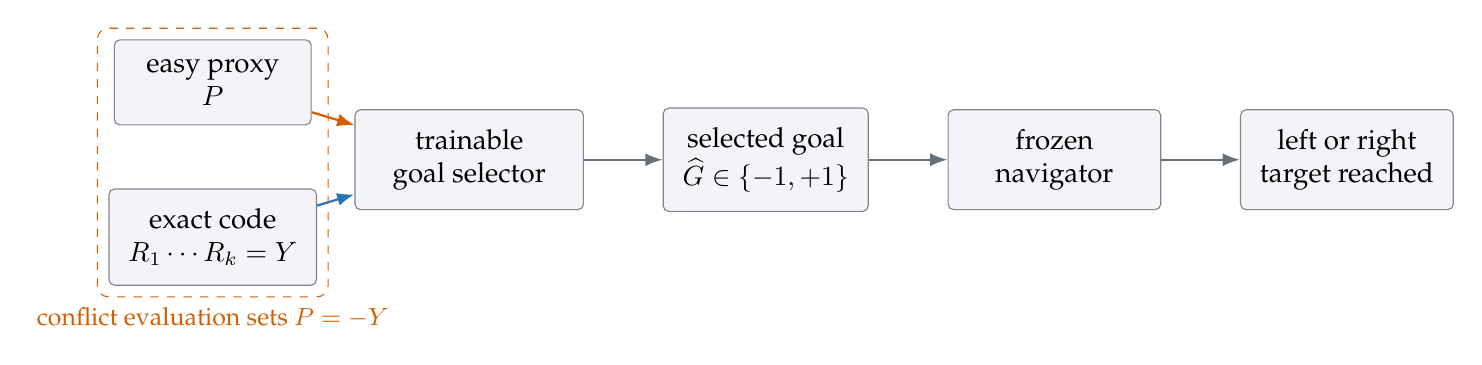
\begin{tikzpicture}[
    node distance=8mm and 10mm,
    box/.style={draw=ink!55, rounded corners=2pt, fill=softgray, inner sep=7pt, align=center, minimum height=9mm},
    sig/.style={box, minimum width=25mm},
    arrow/.style={-{Latex[length=2.2mm]}, thick, draw=ink!65}
  ]
    \node[sig] (proxy) {easy proxy\\$P$};
    \node[sig, below=of proxy] (exact) {exact code\\$R_1\cdots R_k=Y$};
    \node[box, right=18mm of $(proxy)!0.5!(exact)$, minimum width=29mm] (selector) {trainable\\goal selector};
    \node[box, right=of selector, minimum width=26mm] (goal) {selected goal\\$\widehat G\in\{-1,+1\}$};
    \node[box, right=of goal, minimum width=27mm] (nav) {frozen\\navigator};
    \node[box, right=of nav, minimum width=25mm] (target) {left or right\\target reached};
    \draw[arrow,proxy] (proxy) -- (selector);
    \draw[arrow,intended] (exact) -- (selector);
    \draw[arrow] (selector) -- (goal);
    \draw[arrow] (goal) -- (nav);
    \draw[arrow] (nav) -- (target);
    \node[draw=proxy, dashed, rounded corners, fit=(proxy)(exact), inner sep=4pt,
          label={[proxy]below:{\small conflict evaluation sets $P=-Y$}}] {};
  \end{tikzpicture}
  }
  \caption{\textbf{The experimental separation.} The selector sees a simple proxy and an exact interaction code. Navigation is pretrained and frozen, so changing the selected destination need not relearn how to move. The full factorial analysis is conducted at the one-step choice level; fork and navigation rollouts confirm that the same selector can drive sequential behavior on maps within the navigator's support.}
  \label{fig:forkworld}
\end{figure}

The original experiments run the same learned selector at three levels: a one-step contextual choice, a gridworld with one meaningful fork, and a fuller navigation environment. The clean causal estimates come from the first. The latter two ask whether a single selected goal can be handed to a competent frozen controller without changing the result (\fig{fig:forkworld}). They are support-map confirmations, not evidence of general navigation: the frozen navigator performs poorly on held-out map layouts. A later RouteWorld experiment instead makes the selector choose at several reward-relevant forks inside a walled maze, while a scripted controller handles forced corridor moves. This adds repeated goal decisions without conflating them with learned path planning.

The main results below are organized around the patterns in the data. All uncertainty intervals resample the ten independent training seeds; exploratory and post-hoc labels describe selection status, not a different interval calculation. In the one-step families, the 10,000 evaluation states per run make each trained policy's behavior easy to measure; they do \emph{not} turn one trained seed into 10,000 independent replicates. Route branches and physical rollouts are likewise repeated measurements of a trained seed, not additional independent replicates.

\section*{Finding 1: Near-perfect performance can conceal the wrong goal}

On an example where $P=Y$, the proxy and intended rules predict the same action. Such an example can teach the action, but it contributes no evidence for \emph{which explanation} is controlling the model. If $N$ training examples contain only
\[
N_{\mathrm{conflict}}=N(1-q)
\]
proxy failures, then the exact rule's entire advantage is concentrated in those examples. A direct readout of $P$ can reduce most of the loss immediately; a degree-$k$ interaction must pay a larger optimization cost to recover the residual.

Viewed this way, the relevant tradeoff is more specific than a universal ``simplicity bias'': a signal wins when its predictive improvement is large relative to the effective cost of extracting it. Thus ``sufficiently accurate'' is not one value of $q$; it is a surface in proxy reliability, rule complexity, architecture, update budget, and training time.

Controlled simplicity-bias experiments have likewise found that gradient-trained networks can rely exclusively on the simplest predictive feature, even when more complex features are more accurate \citep{shah2020pitfalls}. Related work on gradient starvation shows how progress along one predictive route can suppress learning along another \citep{pezeshki2021gradient}. \Forkworld{} extends those comparisons by measuring which feature retains causal control when the two rules are forced to recommend opposite actions.

\subsection*{Experiment and result}

To map this tradeoff, we trained two-layer ReLU selectors on 10,000 examples for 2,048 optimizer steps, sweeping
\[
q\in\{.50,.60,.70,.80,.90,.95,.99,1\},\quad
k\in\{1,2,3,4,5\},
\]
and widths $8,16,32,64,128$, with ten seeds per cell: 2,000 completed runs. The phase boundary in \fig{fig:phase}, panel a, is sharp. Increasing proxy accuracy strongly shifts behavior toward the proxy: the seed-wise Spearman effect on $\rhoY-\rhoP$ is $-0.663$, 95\% \CI{} $[-0.676,-0.648]$. Increasing $k$ also favors the proxy ($-0.212$, $[-0.232,-0.194]$). Capacity moves in the intended direction, but the pooled effect is much smaller ($+0.071$, $[+0.053,+0.091]$) because most easy cells are already saturated.

At the high-accuracy edge, the phase boundary becomes especially clear. At $q=.99$, mean $\rhoY$ for $k=1,\ldots,5$ is $1.000,1.000,.924,.615,.117$. A width-8, $k=5$ model obtains 99\% in-distribution accuracy while following the proxy on every conflict input ($\rhoY=0$). At $q=1$, every model with $k\geq2$ has perfect training-distribution accuracy and $\rhoY=0$, at every tested width. Perfect performance leaves the goal entirely unidentified.

The same interpretation is supported by causal feature-flip interventions. Among policies with $\rhoY\leq.1$, flipping only $P$ flips the hard decision 99.7\% of the time, whereas flipping an $R_i$ does so 0.3\% of the time. Among policies with $\rhoY>.9$, those rates reverse to 0.1\% and 99.9\%. Conflict performance is therefore not just correlated with a proxy label; it tracks which channel actually controls the action.

\begin{takeaway}
Training accuracy measures how often candidate goals agree with the labels. It cannot identify the learned goal unless training or evaluation contains states where those goals recommend different actions.
\end{takeaway}

\begin{figure}[!htbp]
  \centering
  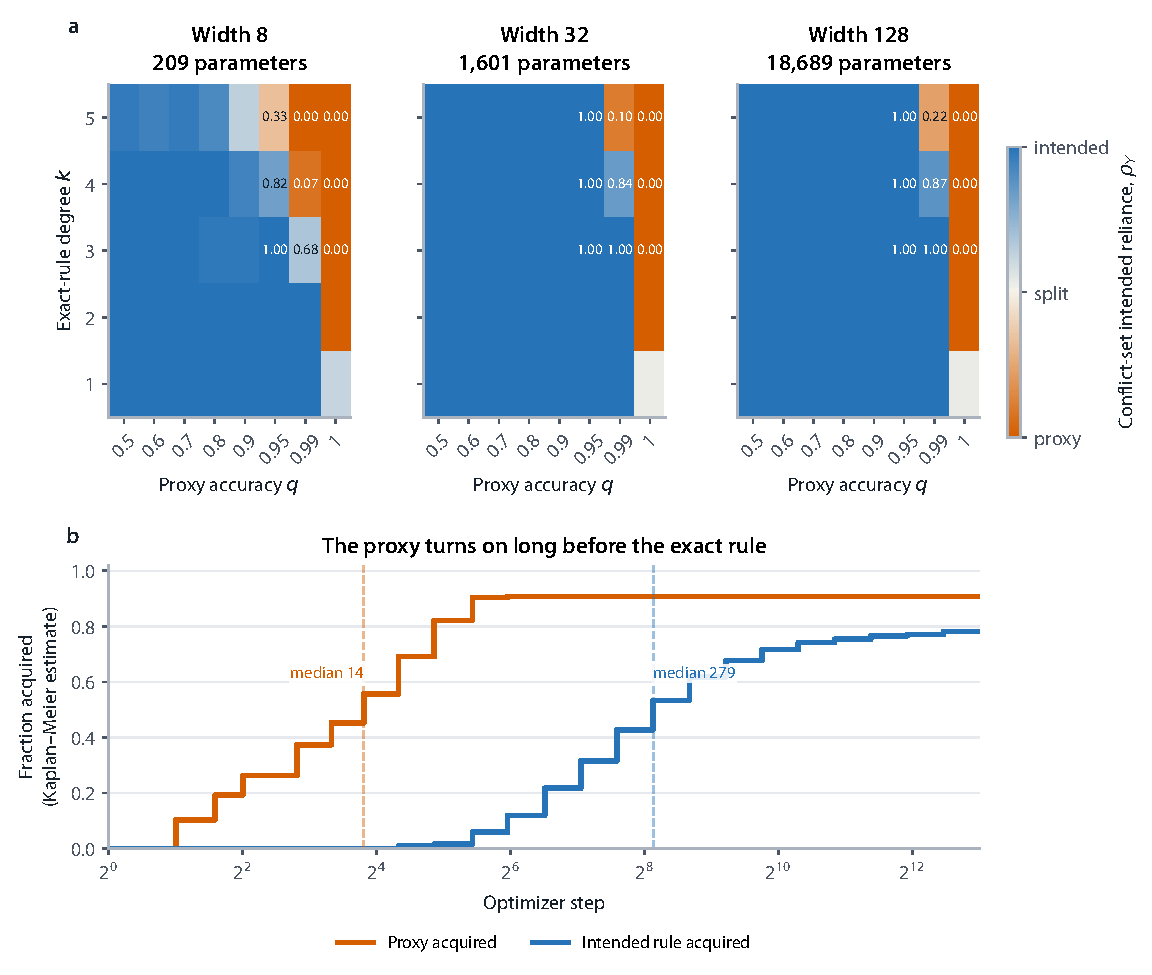
\includegraphics[width=\linewidth]{fig1_phase_and_dynamics.pdf}
  \caption{\textbf{Proxy and intended-rule acquisition across accuracy, complexity, and training time.} \textbf{a}, Mean intended-goal reliance at three representative widths (ten seeds per cell). Orange denotes proxy control and blue intended control. The complete sweep also contains widths 16 and 64. At $q=1$, all $k\geq2$ cells are proxy-controlled despite perfect in-distribution accuracy. \textbf{b}, Kaplan--Meier acquisition curves over all 2,400 training-dynamics runs. Acquisition means $\rho\geq.9$ at two consecutive logged checkpoints. Curves pool heterogeneous factorial conditions descriptively; confirmatory ordering uses seed-level resampling. Median proxy and intended acquisition times are 14 and 279 optimizer steps.}
  \label{fig:phase}
\end{figure}

\section*{Finding 2: Models learn the simple proxy first---and accumulated counterexamples can make them abandon it}

The proxy has an immediate gradient: a model can improve by placing weight on one observed coordinate. The exact parity rule needs several features to become useful together. Early training should therefore look like
\[
\text{no stable rule}\;\longrightarrow\;\text{proxy}\;\longrightarrow\;\text{intended rule}.
\]
The last arrow is not automatic. Once the proxy is learned, the agreement examples are nearly solved and the remaining corrective gradient is concentrated on its mistakes. If those mistakes continue to recur, the model has a reason to build the harder computation. If they are absent, too rare, or too homogeneous, proxy reliance can lock in.

The proxy-first part of this picture is consistent with earlier observations that neural networks prioritize simple patterns and that spurious features can become visible very early in training \citep{arpit2017memorization,yang2024spurious}. The later replacement resembles delayed generalization, or grokking, in which a structured rule emerges after a model has already fit its training data \citep{power2022grokking,nanda2023progress}. Here the transition is between causally measured decision rules, and, as we show below, it usually does not occur long after training reward has plateaued.

\subsection*{Experiment and result}

To observe this sequence directly, the training-dynamics experiment saved 25 logarithmically spaced checkpoints over 8,192 updates on the factorial grid
\[
\begin{gathered}
q\in\{.60,.80,.90,.95,.99\},\qquad k\in\{2,3,4,5\},\\
N\in\{1{,}000,4{,}000,16{,}000\},\qquad w\in\{16,32,64,128\}.
\end{gathered}
\]
Acquisition required reliance at least .9 at two consecutive checkpoints.

The acquisition order is identifiable in 2,399 of 2,400 runs. The seed-weighted simple-first fraction is .9083, 95\% \CI{} $[.8945,.9213]$. More strongly, in all 1,655 runs where both goals cross threshold, the proxy is first. The remaining identifiable cases are mostly one-sided censoring: 524 acquire only the proxy and 220 only the intended rule. Among runs where both are observed, intended acquisition lags proxy acquisition by 471.7 steps on average ($[459.2,485.4]$). Panel b of \fig{fig:phase} shows the corresponding median separation.

The shorter phase-diagram runs supply the clearest behavioral unlearning contrast. Of 1,291 runs that first acquire the proxy, 76.1\% later undergo sustained proxy-to-intended replacement by step 2,048. Conditional replacement falls from 99.3\% at $q=.60$ to 90.3\% at $q=.95$, 62.0\% at $q=.99$, and zero at $q=1$. Merely moving from $q=1$ to $.99$---from zero to 100 proxy errors in a 10,000-row dataset---raises final $\rhoY$ by .619 ($[.591,.642]$).

Here, ``unlearning'' means that negative training evidence removes the proxy's causal control over the final choice and replaces it with the exact rule; it need not erase every internal representation of $P$.

\subsection*{Reward and goal identity usually stabilized together}

We had also predicted that training reward would usually plateau before goal identity stabilized, but only 13.2\% of identifiable runs plateau first ($[12.5\%,14.0\%]$): 302 plateau first, 606 stabilize the goal first, and 1,372 tie at the same logged checkpoint. Thus the joint prediction fails even though the proxy-first component is strongly supported.

In this supervised toy task, the residual $1-q$ error is clean enough that learning the intended rule visibly improves training performance at roughly the same measurement time. The result also warns against turning the cross-sectional observation that equal accuracy can hide different goals into a stronger temporal claim that reward always stabilizes long before the goal changes. Checkpoints are logarithmically spaced and the plateau statistic uses a four-checkpoint window, so the 1,372 ties also reflect coarse temporal resolution.

\section*{Finding 3: Distinct counterexamples---not raw repetition---identify the intended goal}

Imagine maintaining a set of rules consistent with the data. An agreement example eliminates neither $P$ nor $Y$. One conflict example eliminates the pure proxy rule, but a flexible network can retain it globally and store that state as an exception. Repeating the same exception raises its weight in the loss without adding a new constraint. A collection of conflicts spread across locations, geometries, and nuisance values is harder to explain away; the compact solution is increasingly the intended rule itself.

In likelihood language, agreement examples have a likelihood ratio near one between the two candidate goals. Conflict examples move that ratio. But even the conflict \emph{count} is incomplete: generalization depends on how many independent ways the proxy has been shown to fail.

Counterfactually augmented datasets try to create precisely this kind of distinguishing evidence by changing inputs so that the label reverses while irrelevant details remain fixed \citep{kaushik2020difference}. Recent work describes a particularly relevant failure mode: a network can retain a simple majority explanation while memorizing the exceptions, reaching zero training loss without learning the robust rule \citep{bayat2025pitfalls}. The experiment below isolates whether adding distinct conflicts helps beyond repeating the same conflicts more often.

\subsection*{Separating conflict count from diversity}

An exploratory re-analysis of the training-dynamics runs first groups models by the number of conflict rows available in their finite training dataset. Exact-rule acquisition rises steeply with that number, and the required amount increases with $k$ (\fig{fig:evidence}a). At 100 conflict rows, all $k=2$ and $k=3$ runs acquire the intended rule, but only 55\% of $k=4$ and none of $k=5$ do. At 400 rows, the corresponding fractions are essentially one for every $k$ (99\% for $k=5$). Frequency still affects speed: at matched conflict counts, larger $q$ exposes those rows less often per update and delays acquisition.

The matched-diversity experiment then performs the causal comparison. It fixes $N=10{,}000$ and, within each comparison, fixes $N_{\mathrm{conflict}}$, $q$, and $k$, while varying the fraction of conflict presentations that are unique: 2\%, 10\%, 50\%, or 100\%. Models are evaluated only on unseen conflict contexts. A structured-holdout arm trains on location reflection and coordinate exchange but tests geometry rotation and nuisance inversion; the failure-mechanism identity is hidden from the model. The grid covers six conflict counts, five values of $k$, and ten seeds (1,500 runs).

The mean diverse-minus-concentrated effect is +.2988, 95\% \CI{} $[.2895,.3082]$. All 24 estimable fixed-count/$k$ strata show a positive diversity association; the median within-stratum Spearman correlation is .855. Agreement-only training yields $\rhoY=.1102$ ($[.0892,.1346]$), far below the .9 acquisition criterion. With fully diverse conflicts, the first tested count whose mean reaches .9 is 32 for $k=1$, 128 for $k=2,3$, and 512 for $k=4,5$.

\begin{figure}[!t]
  \centering
  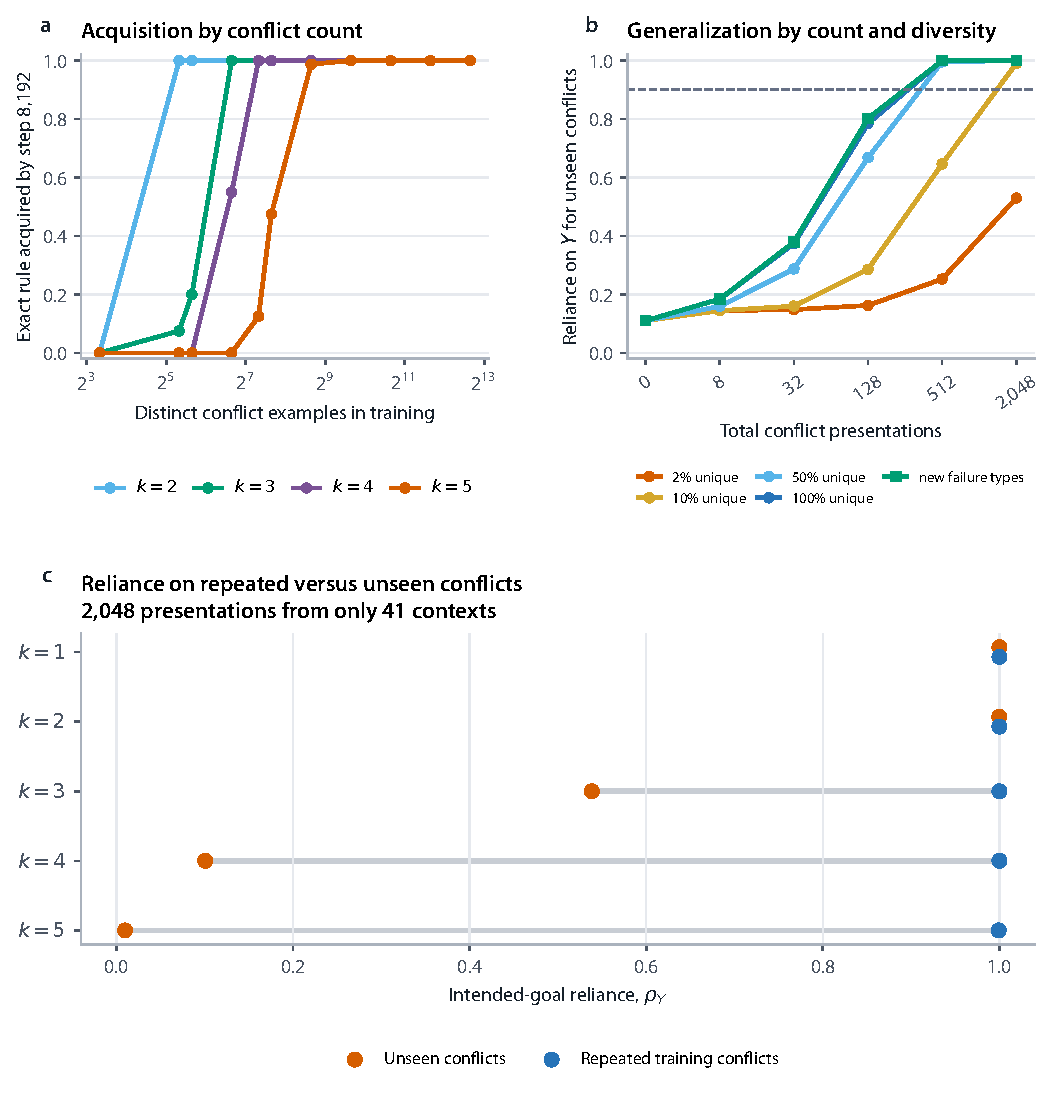
\includegraphics[width=\linewidth]{fig2_counterevidence.pdf}
  \caption{\textbf{Effects of conflict count and diversity on intended-goal reliance.} \textbf{a}, Exploratory acquisition probability versus the number of available conflict examples, split by exact-rule degree. \textbf{b}, Intended-goal reliance on unseen conflicts, averaged over $k=1,\ldots,5$. Every contrast at a fixed x-position matches total conflict count and proxy accuracy; only the unique-context fraction changes. ``New failure types'' is the structured holdout. \textbf{c}, With 2,048 conflicts but only 41 distinct contexts, all degrees fit repeated training conflicts almost perfectly, while high-degree models follow the proxy on novel conflicts.}
  \label{fig:evidence}
\end{figure}

\subsection*{A model can fit every counterexample and still infer the wrong goal elsewhere}

In the most concentrated cell, 2,048 of 10,000 rows are conflicts, so the proxy is wrong on 20.48\% of training data, but only 41 conflict contexts are distinct. At $k=5$, the model follows $Y$ on 99.92\% of repeated training conflicts, yet on unseen conflicts $\rhoY=.0098$. Flipping $P$ changes 98.39\% of its decisions. The model has not failed to fit the negative evidence. It has learned a catalog of exceptions while retaining the proxy as its general rule.

A structured-holdout control performs within half a percentage point of a matched fully diverse arm: structured minus matched-diverse $=+.0046$ ($[.0026,.0065]$). We interpret this as practical parity, not as a meaningful benefit. Within this synthetic transform family, sufficiently varied errors transfer to new kinds of failure rather than requiring the model to memorize each named corruption.

\begin{takeaway}
When auditing goal generalization, count distinct, representative disagreements between plausible goals. A large dataset or a large number of repeated failures can badly overstate how much evidence actually identifies the intended rule.
\end{takeaway}
\FloatBarrier

\section*{Finding 4: Being able to decode a goal is not the same as selecting it}

A standalone decoder asks, ``Can this architecture learn $Y$ when $Y$ is the only target?'' Goal competition asks a different question: ``Will optimization allocate enough of its update to $Y$ when one observed coordinate already buys 90\% accuracy?'' Let
\[
C_{\mathrm{decode}}(Y)
\]
be the update capacity needed to read the exact code in isolation, and let
\[
C_{\mathrm{win}}(Y\mid P)
\]
be the capacity needed for it to control behavior in the presence of $P$. There is no reason these thresholds must coincide. The second includes an opportunity cost, a gradient-allocation problem, and interaction with whatever route makes $P$ easy.

The distinction between information that is encoded and information that a model actually uses is a known interpretability trap: high probing accuracy need not imply relevance to the model's task \citep{ravichander2021probing}. Amnesic probing and causal mediation address this by intervening on candidate information and measuring the behavioral effect \citep{elazar2021amnesic,vig2020causal}. \Forkworld{} applies the same distinction to candidate objectives and separately calibrates representability before testing control under competition.

\subsection*{Experiment and result}

To distinguish accessibility from behavioral control, we train three separate models for every architecture and update restriction, keeping the input interface and parameter count fixed: a proxy-only calibration, an exact-code-only calibration, and a $P$-versus-$R$ competition model at $q=.9$. We sweep depth, width, activation, residual connections, full updates, head-only updates, and random parameter subspaces. The subspace restriction adapts the intrinsic-dimension method of training in a fixed random projection of parameter space \citep{li2018intrinsic}. There are 9,300 completed runs.

Crossing the exact-calibration threshold predicts greater intended-goal reliance, but does not determine it. Competition $\rhoY$ is higher by .810 for full updates ($[.648,.948]$), .310 for head-only updates ($[.293,.326]$), and .211 for subspace updates ($[.180,.240]$) after the crossing. Yet the subspace thresholds are widely separated:

\begin{center}
\begin{tabular}{lccccc}
\toprule
Exact-rule degree & $k=1$ & $k=2$ & $k=3$ & $k=4$ & $k=5$ \\
\midrule
$C_{\mathrm{decode}}$ & 16 & 16 & 64 & 64 & 256 \\
$C_{\mathrm{win}}$ & 64 & 256 & 1,024 & 1,024 & $>1{,}024$ \\
\bottomrule
\end{tabular}
\end{center}

These are first crossings on the tested grid, using final decoder accuracy at least .95 or behavioral $\rhoY\geq.9$ in at least eight of ten seeds. At $k=3,U=64$, the standalone decoder is perfect but competition $\rhoY=.001$. At $k=4,U=256$, decoder accuracy remains 1 while $\rhoY=0$. At $k=5,U=1024$, the decoder is again perfect but $\rhoY=.102$ (\fig{fig:decode}a). A readable goal can remain behaviorally inert.

\begin{figure}[!htbp]
  \centering
  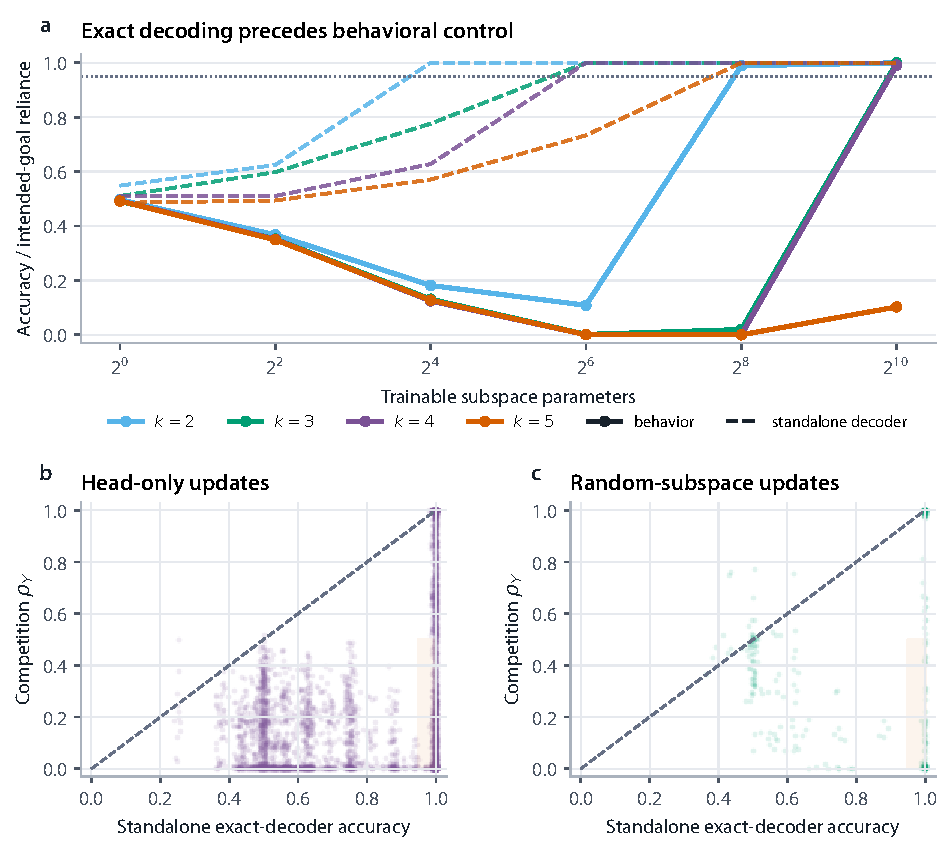
\includegraphics[width=\linewidth]{fig3_decoding_vs_control.pdf}
  \caption{\textbf{Decodability precedes control, sometimes by orders of magnitude in update size.} \textbf{a}, Standalone exact-decoder accuracy (dashed) and competition reliance (solid) for random-subspace updates. At intermediate budgets, the decoder has solved parity while the competing policy is more reliably proxy-controlled than at initialization. \textbf{b--c}, Seed-level calibration and competition outcomes for head-only and subspace updates. Points far below the diagonal are decodable-but-not-controlling cases. Jitter is visual only. The orange rectangle marks decoder accuracy above .95 with competition reliance below .5.}
  \label{fig:decode}
\end{figure}

\subsection*{The architecture can change which goal wins without changing parameter count}

For example, full-training, depth-4, width-8 tanh models have exactly 353 parameters and perfect exact decoders with or without a residual connection. At $k=5$, however, the non-residual model has $\rhoY=.420$, while the residual model has $\rhoY=1.000$; the paired difference is $-.580$ ($[-.772,-.369]$). Similar gaps appear at $k=3$ and $k=4$. Meanwhile GELU and ReLU non-residual models at the same parameter count reach $\rhoY=1$.

Across 1,170 preregistered matched-parameter architecture pairs, 267 show interval-supported differences in both decoder and behavior. Only 111 differences point in the same direction; 156 point oppositely. Those aggregate pair counts are exploratory and not corrected for multiple comparisons, but they suggest that architecture affects the optimization geometry of competition, not only what can be represented.

\section*{Finding 5: Low-order clues, not channel count, predict which exact rules can beat a 99\%-accurate proxy}

Counting inputs is an appealing way to rank rules: a direct feature looks simple, while a rule involving five or six features looks complex. Neural networks do not experience complexity as an input count, however. A majority rule gives a useful clue whenever one of its inputs is revealed; a conjunction is mostly recognizable from a single negative input; and a multiplexer first has to route an address but then copies one data bit. Parity is different. Every strict subset of its bits is exactly uninformative, so a learner receives no reliable partial solution on the way to assembling the full interaction. This distinction is familiar in work on learning Boolean functions and high-degree parities, where learnability depends on the function and optimization path rather than only on representation size \citep{malach2019boolean,abbe2025parities}.

We therefore expected the earlier ``degree'' effect to be partly an effect of parity's information structure. If so, replacing parity with other exact rules should change which goal wins even when the number of visible channels, training exposure, architecture, and proxy reliability are held fixed.

\subsection*{Matched exact-rule competition}

We compare four balanced encodings: five-bit parity, five-bit majority, five-bit conjunction, and a six-bit multiplexer whose two address bits select one of four data bits. Padding fixes every selector's input interface at six rule channels. For each rule we cross proxy accuracy $q\in\{.75,.9,.99\}$, widths $8$ through $128$, one or two hidden layers, and ten seeds. Each of the 1,200 runs trains a proxy-only decoder, an exact-rule-only decoder, and a competition model on the same architecture for 4,096 updates.

The interventions are defined at the rule level rather than by casually comparing one coordinate across unlike functions. For every evaluation row, a minimum-Hamming counterfactual changes just enough active rule bits to force the decoded value from $Y$ to $-Y$. We also estimate the best possible prediction from each individual channel. The latter is near chance for parity, but need not be for the other rules; that lower-order signal is a feature of the comparison rather than an unmeasured confound.

\subsection*{Useful partial evidence changes which exact rule wins}

All four encodings are accessible in isolation at nearly every tested architecture. Mean standalone accuracy is .993 for parity and 1.000 for the other three; after excluding width eight, every final exact decoder has measured accuracy 1.000. Their behavior in competition nevertheless separates sharply at the 99\%-accurate proxy boundary (\fig{fig:rules}). Mean conflict-set intended reliance is .100 $([.067,.137])$ for parity, .885 $([.870,.901])$ for the multiplexer, .985 $([.971,.996])$ for conjunction, and 1.000 for majority. IID accuracies remain at least .991, so an ordinary validation set makes these policies look nearly interchangeable.

The causal counterfactual supports the behavioral interpretation. Whole-rule flip rates closely track conflict reliance, while proxy flips dominate the parity models that fail. Across all matched cells, majority, conjunction, and multiplexer increase intended reliance over parity by .345 $([.325,.366])$, .340 $([.319,.360])$, and .306 $([.286,.326])$, respectively. Their advantage in final standalone decoder accuracy is only .0066. The much larger control gap therefore cannot be summarized as ``one decoder eventually reached a slightly higher score.''

The lower-order measurements offer a correlational account of the ordering. On the training distribution, the best empirical single-channel Bayes accuracies average .507 for parity, .628 for the multiplexer, .693 for majority, and .763 for conjunction. At $q=.99$, their within-seed rank correlation with intended reliance is .788 $([.736,.832])$. An exploratory timing summary also finds much earlier standalone acquisition: using a .95 threshold with two-checkpoint persistence and coding non-crossers at the 4,096-update horizon, the restricted mean first-crossing time is 35 updates for majority, 53 for conjunction, 123 for the multiplexer, and 491 for parity. Seven of 100 unique parity controls remain censored. At $q=.99$, every majority and conjunction competition run crosses the registered .9 acquisition threshold, compared with 26 of 100 multiplexer runs and none of the parity runs.

An exploratory depth-by-width contrast does not restore a monotonic story. For the $q=.99$ multiplexer, moving from one to two hidden layers helps by .124 at width eight but hurts by .121 at width 128; the paired difference-in-differences is $-.245$ $([-.304,-.188])$. Because exposure and optimizer steps are fixed, this interaction is evidence about optimization and implicit bias, not a claim that fewer parameters are generally better.

\begin{figure}[!htbp]
  \centering
  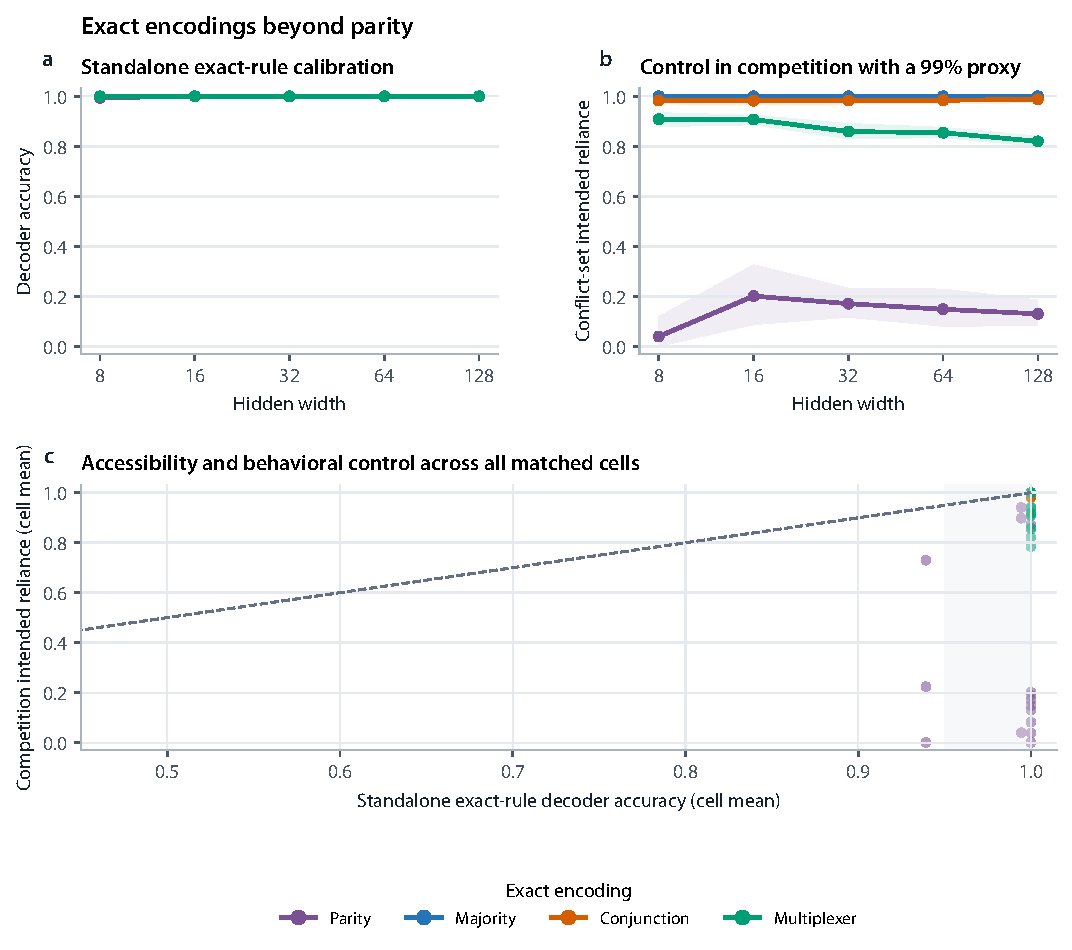
\includegraphics[width=\linewidth]{fig11_rule_families_followup.pdf}
  \caption{\textbf{The number of exact-rule inputs does not determine whether that rule controls behavior.} \textbf{a}, Standalone calibration is essentially perfect for all four encodings. \textbf{b}, With a 99\%-accurate direct proxy, majority and conjunction retain intended control, the multiplexer is intermediate, and parity is usually proxy-controlled. Lines show ten-seed means at depth two; bands show 95\% seed-bootstrap intervals. \textbf{c}, Final decodability is compressed near one while competition outcomes span the full range across both tested depths. The dashed diagonal marks equality between standalone accuracy and conflict-set intended reliance.}
  \label{fig:rules}
\end{figure}

These four fixed functions do not establish a universal ordering over Boolean rules. They show why ``number of channels'' was never a portable definition of goal complexity. Parity was useful precisely because it removes partial clues; majority and conjunction change both the computation and the marginal gradient information available before the full rule is learned. The association therefore does not isolate a unique mechanism. A prediction about which goal wins nevertheless needs a model-relative account of the rule's learning path, not only a symbolic description length.

\begin{takeaway}
Parity is a particularly severe shortcut-learning test. Equal-sized exact encodings with useful lower-order evidence can defeat a 99\%-accurate direct proxy even when parity does not.
\end{takeaway}

\section*{Finding 6: A little update capacity can make the model more capable---and more wrong}

At initialization, neither candidate rule controls behavior, so conflict accuracy is near chance. The first useful capacity may be enough to exploit the one-coordinate proxy but not enough to build parity. In-distribution performance then improves while conflict behavior gets \emph{worse}. Only a later capacity threshold makes the intended computation win:
\[
\text{neither rule}\;\longrightarrow\;\text{proxy only}\;\longrightarrow\;\text{intended rule}.
\]
This produces a miniature inverse-scaling curve. It does not imply that capacity is intrinsically harmful. It says that capabilities arrive in an order, and the earliest accessible capability can be the wrong generalization.

\subsection*{Update-capacity sweeps}

The random-subspace sweep shows the full dip in \fig{fig:decode}a. From $U=1$ to $U=16$, mean $\rhoY$ falls from .497 to .182 for $k=2$, .491 to .131 for $k=3$, .493 to .125 for $k=4$, and .492 to .127 for $k=5$. All paired intervals exclude zero. The proxy has become reliable before parity is competitive. At $U=256$, $k=2$ jumps to .989; at $U=1024$, $k=3$ reaches 1 and $k=4$ reaches .992; $k=5$ remains proxy-controlled at .102.

The algorithm comparison independently reproduces the same first transition. Under clean SFT, increasing $U$ from 1 to 64 raises in-distribution target accuracy from .511 to .900 while conflict $\rhoY$ falls from .491 to .0004. At $U=256$, the intended rule begins to return ($\rhoY=.486$); at $U=1024$, it takes complete control. RL follows almost the same decline through $U=64$ but, in this experiment, never makes the second transition (\fig{fig:algorithms}).

Taken together, the two capacity sweeps show that a model can become more consistent, more accurate, and easier to deploy while simultaneously becoming more predictably wrong in the states that reveal its objective.

\section*{Finding 7: In this Forkworld, SFT escapes the proxy; RL reinforces it---even with every actor weight trainable}

Signal separation offers one proposed explanation for the extreme update efficiency of RL \citep{morris2026reason}. An SFT demonstration specifies many token-level or action-level choices. Some are essential to success and others are incidental. A tiny update may spend capacity reproducing all of them. RL instead observes whether a sampled trajectory succeeds. Across fresh trajectories, effects consistently associated with reward accumulate, while reward-irrelevant variation can cancel.

Signal separation does not imply an automatic RL advantage. If SFT receives a clean action label, it has a dense, low-entropy target and may be more efficient than terminal-reward RL. An RL advantage should be largest when demonstrations contain many nuisance choices that are irrelevant to reward.

\subsection*{Experiment}

We test this comparison using four algorithms on the same 5,897-parameter actor at $q=.9,k=3$: clean action SFT, nuisance-rich trajectory SFT, on-policy imitation with the same clean oracle, and RL with a fixed oversized critic. The on-policy arm separates reward learning from learner-induced state-distribution shift, the motivation behind no-regret imitation methods such as DAgger \citep{ross2011reduction}. Actor updates are restricted to $U\in\{1,4,16,64,256,1024,\text{full}\}$ trainable scalars. Trajectories contain zero, two, four, or eight fair binary branch choices, resampled on every presentation. Every arm receives 2,048 updates of batch size 250, or 512,000 presentations. The success threshold is $\rhoY\geq.9$ in at least eight of ten seeds.

\subsection*{Result and interpretation}

At $U=1024$, clean SFT and trajectory SFT have $\rhoY=1$ at every nuisance entropy. On-policy imitation averages .920, with eight of ten seeds above threshold. RL has $\rhoY=0$ at every entropy and flipping $P$ flips essentially every decision. Its in-distribution accuracy is exactly .900: it has found the 90\%-accurate proxy.

Even with every actor weight trainable, RL remains at $\rhoY=0$ when nuisance entropy is zero; at $H=2,4,8$, it reaches only $.076,.074,.100$. At $H=8$, trajectory SFT minus RL is .900 ($[.824,.975]$). On-policy imitation also succeeds at $U=1024$, so the RL failure is not reproduced merely by moving SFT onto the current policy's state distribution.

\begin{figure}[!htbp]
  \centering
  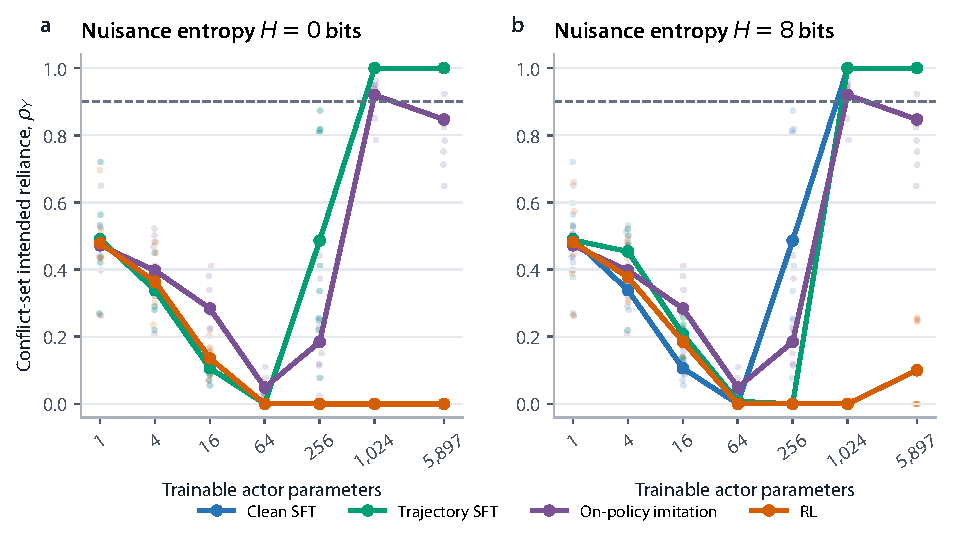
\includegraphics[width=\linewidth]{fig4_update_capacity.pdf}
  \caption{\textbf{Update capacity first installs the proxy, then lets SFT replace it; RL never crosses the second boundary.} Dots are seed-level outcomes and lines are seed means. Clean and trajectory SFT overlap at $H=0$; clean SFT is an exact control duplicate across nuisance settings. ``Full'' uses all 5,897 actor parameters, while smaller budgets use a random-subspace parameterization, so the x-axis changes update geometry as well as dimension. The dashed line is the .9 success threshold.}
  \label{fig:algorithms}
\end{figure}

Because RL never crosses the threshold on the tested grid, the comparison is weaker than the visual reversal might suggest. Clean and trajectory SFT first cross at $U=1024$, while RL's threshold is right-censored above 5,897. Thus
\[
\frac{U_{\min}^{\mathrm{trajectory}}}{U_{\min}^{\mathrm{RL}}}
<\frac{1024}{5897}=0.174,
\]
but every bootstrap draw for the two-sided threshold ratio is censored. The data establish a one-sided bound, not a finite two-sided threshold ratio.

The nuisance construction also limits construct validity. The nuisance branch labels are hidden from the observation and freshly resampled. Their population-optimal prediction is one half, and the nuisance heads remain at chance. This manipulation injects irreducible label and gradient noise; it does not force SFT to learn a rich, context-predictable but reward-irrelevant structure of the sort found in language demonstrations. Indeed, nuisance entropy leaves the tested SFT threshold at 1,024, though it changes behavior below threshold. The comparison therefore shows that RL has no generic immunity to proxy lock-in in this Forkworld. It does \emph{not} rule out an RL update-capacity advantage on richer reasoning traces, nor does one shared hyperparameter schedule establish the best possible RL result.

\section*{Finding 8: Entropy pressure moves the RL shortcut boundary, but does not erase it}

Policy-gradient learning can make an early success self-reinforcing. Once a policy assigns nearly all probability to the action predicted by a good proxy, it rarely samples the alternative action and receives little direct information about what that action would have earned. Entropy regularization modifies the objective to reward a less concentrated policy,
\[
J_\beta(\pi)=\mathbb{E}[R]+\beta\,\mathbb{E}[\mathcal H(\pi)],
\]
which can delay saturation and change the optimization path \citep{ahmed2019entropy,husain2021regularized}. In this experiment every context is sampled regardless of the action, so this is not exploration in the sense of discovering new map states. It is stochastic action exploration combined with a change to the objective geometry.

We expected entropy pressure to help only where the intended computation was learnable but the proxy captured the policy too early. If the rule is already easy, there is no trap to escape; if it is inaccessible, randomizing actions cannot create a decoder; and if the proxy is almost perfect, the reward advantage of the intended rule may be too rare.

\subsection*{Sweeping the policy's resistance to collapse}

The follow-up crosses proxy accuracy $q\in\{.5,.75,.9,.99\}$, parity degree $k\in\{2,3,4\}$, and entropy coefficient $\beta\in\{0,.003,.01,.03,.1,.3\}$ for ten seeds: 720 full actor--critic runs. At the canonical $q=.9,k=3$ cell we repeat the sweep with REINFORCE and with a 1,024-scalar actor update subspace, adding 120 runs. Every policy receives 2,048 updates and is evaluated greedily. The $q=.5$ cells are a falsifier: without a useful proxy, failure to learn parity would indicate a general RL capability limit rather than proxy lock-in.

The registered mechanism-panel trigger required some entropy coefficient at the canonical full actor--critic cell to improve mean conflict reliance by at least .20, with a paired interval above zero. This threshold was fixed before the sweep; it prevents a visually interesting cell elsewhere from silently redefining the planned test.

\subsection*{The response is localized and non-monotonic}

Across the full primary grid, $\beta=.3$ raises intended reliance over $\beta=0$ by only .056 $([.034,.079])$. At the canonical $q=.9,k=3$ cell, $\beta=.1$ changes $\rhoY$ from zero to .125 $([.050,.200])$ and $\beta=.3$ changes it to .051 $([0,.126])$. The .20 trigger therefore does not fire. REINFORCE does not show a reliable extra benefit, and the restricted 1,024-scalar actor remains proxy-controlled. Entropy is not a general repair for the RL result above.

Among the 24 registered cellwise contrasts of $\beta\in\{.1,.3\}$ against zero, one harder cell responds much more strongly (\fig{fig:entropy}). At $q=.75,k=4$, raising $\beta$ from zero to .3 moves mean conflict reliance from .050 to .492, a paired gain of .442 $([.248,.667])$; every seed moves in the intended direction. Held-out IID accuracy simultaneously rises from .763 to .873, a gain of .110 $([.062,.163])$. Proxy-flip sensitivity falls from .950 to .508 while exact-rule flip sensitivity rises from .050 to .492. The change is therefore not purchased by random behavior or worse reward: it moves causal control toward the exact rule. Its prominence is selected from the grid, however, and the cellwise interval is not adjusted for that selection.

The improvement is heterogeneous across seeds. Three of ten runs reach $\rhoY>.9$, one reaches roughly .44, and the others cluster near .25. The mean is an optimization-basin shift, not a reliably solved cell. Entropy of the final action distribution on evaluation states is also tiny in both arms ($2.1\times10^{-5}$ versus $.0014$); reliance itself uses greedy actions. Entropy pressure changes how training reaches an almost deterministic endpoint; it does not leave the deployed selector indecisive.

At $q=.5$, the same actor learns degree-two parity perfectly and degree-three parity to .988 even without entropy; degree four rises from .938 to .987 at $\beta=.3$. Conversely, no $q=.99$ cell becomes reliably intended-controlled. Together with the non-monotonic response across $\beta$, this locates entropy's benefit near a narrow boundary where the intended rule is available but not already selected.

\begin{figure}[!htbp]
  \centering
  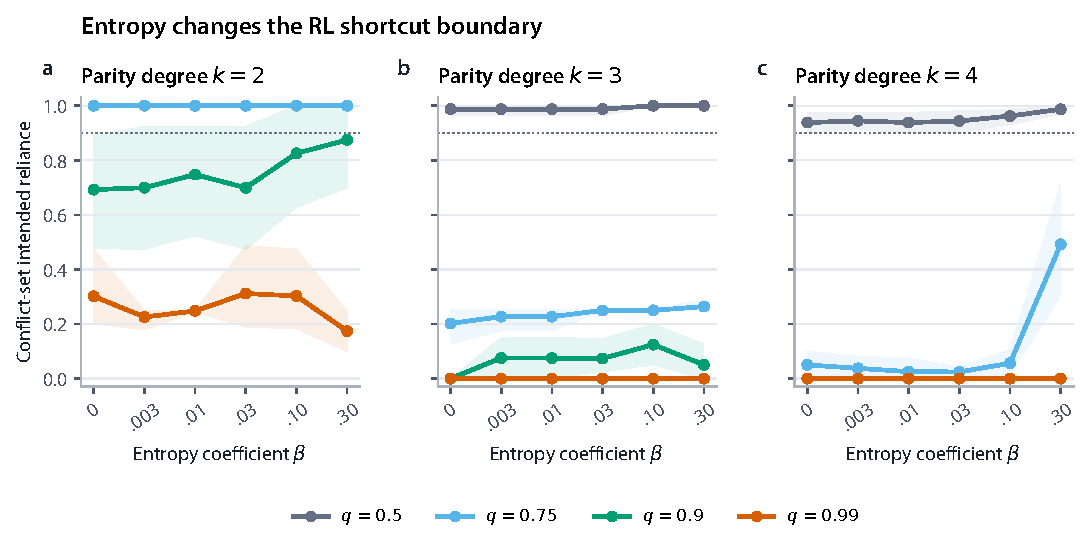
\includegraphics[width=\linewidth]{fig10_rl_entropy_followup.pdf}
  \caption{\textbf{Entropy regularization moves a narrow RL shortcut boundary.} Conflict-set intended reliance is shown across proxy fidelity, parity degree, and entropy coefficient for the full actor--critic. Points are ten-seed means and bands are 95\% seed-bootstrap intervals. The largest response occurs at $q=.75,k=4,\beta=.3$; easier cells are already solved, while no $q=.99$ cell becomes reliably intended-controlled. The dashed horizontal line is the .9 reliability threshold.}
  \label{fig:entropy}
\end{figure}

\begin{takeaway}
Entropy can redirect which goal RL learns, but only in a narrow learnable-yet-captured regime. Its effect is best understood as changing the training trajectory, not as a generic guarantee supplied by exploration.
\end{takeaway}

\section*{Finding 9: Delayed entropy can reopen a saturated proxy policy, usually in discrete truth-table patches}

Entropy can help at two different moments. Applied early, it can keep a policy from becoming so confident in the proxy that the alternative action receives almost no gradient. Applied later, it might ``reheat'' a policy that has already saturated. These mechanisms make opposite timing predictions. If entropy only prevents capture, early exposure should leave a durable benefit and delayed exposure should arrive too late. If its gradient can reopen a collapsed policy, switching it on after capture may still recover intended behavior.

This distinction is especially clean in the contextual bandit. Every semantic context is sampled independently of the action, so delayed entropy does not reveal unexplored parts of a maze. It changes action sampling and the optimization objective after the proxy has already won.

\subsection*{Prevention versus reheating}

We designed this panel only after inspecting the entropy grid above, so every result in this section is exploratory. The registered mechanism-panel trigger at $q=.9,k=3$ did not fire. We instead compare the selected $q=.75,k=4$ responsive cell with the canonical $q=.9,k=3$ comparison cell. Each run trains for 2,048 updates with a boundary after update 64. At that boundary, both zero-entropy and high-entropy policies have essentially zero hard intended reliance in both cells. In the selected cell, however, the high-entropy action distribution remains much softer: mean evaluation entropy is .0822 rather than .0063.

Four schedules form a two-phase factorial: never use entropy, use $\beta=.3$ continuously, use it only for the first 64 updates, or switch it on only for the remaining 1,984. Two additional delayed arms reset either actor Adam or the critic and its optimizer at the boundary without resetting actor weights. Every schedule uses the same ten seeds. The continuous arms exactly reproduce their earlier uninterrupted counterparts; they validate the phase-split implementation but are not independent replications.

\subsection*{Late pressure partially reopens both cells}

Early entropy alone does not prevent proxy capture. In the selected cell, turning it off at update 64 changes final $\rhoY$ by $-.019$ relative to never using it $([-.045,.000])$. By contrast, turning entropy on only after the policy has saturated raises final $\rhoY$ from .050 to .218, a paired gain of .168 $([.111,.222])$; every seed improves, and IID accuracy rises by .041 $([.025,.055])$. Proxy-flip sensitivity falls by the same amount that exact-rule flip sensitivity rises. The policy has changed causal rule control, not merely become less confident.

The canonical comparison cell unexpectedly reheats too. Its never-entropy policy has $\rhoY=0$, while delayed entropy reaches .174, a gain of .174 $([.099,.246])$. Delayed rescue is therefore not specific to the cell selected from the earlier sweep. What differs is the value of exposure during the first 64 updates. With entropy continuing through Phase B, adding early exposure raises final reliance by .274 $([.088,.480])$ in the selected cell but lowers it by .123 $([-.197,-.049])$ in the comparison cell. The across-cell difference between those simple effects is .397 $([.178,.621])$. These supplemental factorial contrasts were chosen during analysis, and they argue against a monotonic ``earlier or more entropy is better'' story.

The component resets do not reliably improve delayed carry. Actor-Adam reset changes the selected-cell endpoint by $+.014$ $([-.025,.053])$ and critic reset by $+.032$ $([-.017,.085])$; both intervals include zero. The corresponding comparison-cell effects also include zero. These controls show that neither tested reset is necessary for partial reheating, though they cannot exclude subtler roles for optimizer or value-state history.

\subsection*{Intermediate means are deterministic patches, not indecision}

Delayed entropy never produces a persistent crossing at or above $\rhoY=.5$. Across delayed carry and the two reset variants, 41 of 60 endpoints finish on the lattice bin at .25 intended reliance. In the carry arm itself, eight of ten selected-cell seeds finish near $4/16$; in the comparison cell, seven finish near $2/8$ and three remain at zero. Continuous entropy in the selected cell is more heterogeneous: six seeds finish near $4/16$, one near $7/16$, and three learn all $16/16$ truth-table rows. Mean final policy entropy is at most .00105 nats in every schedule.

For a confident deterministic policy evaluated uniformly over $k$ binary rule inputs, reliance must lie near $m/2^k$ if the action is constant within each truth-table row. The lattice itself is therefore a support property, not a discovered law. The informative pattern is the concentration at one quarter of the table. All 120 endpoints lie within .01 of a lattice value, with mean absolute residual .0017. Deterministic replays of fixed representative runs confirm the behavioral meaning: a $1/16$ run follows $Y$ on one interaction codeword and $P$ on the other fifteen; a near-$4/16$ run follows $Y$ on three complete codewords and on 99.35\% of a fourth; and a $2/8$ run follows $Y$ on two codewords. This does not identify an internal ``fractional goal.'' It shows that the mean rescue usually consists of nearly deterministic, input-specific patches rather than a stochastic policy choosing the intended action 22\% of the time everywhere.

\begin{figure}[!htbp]
  \centering
  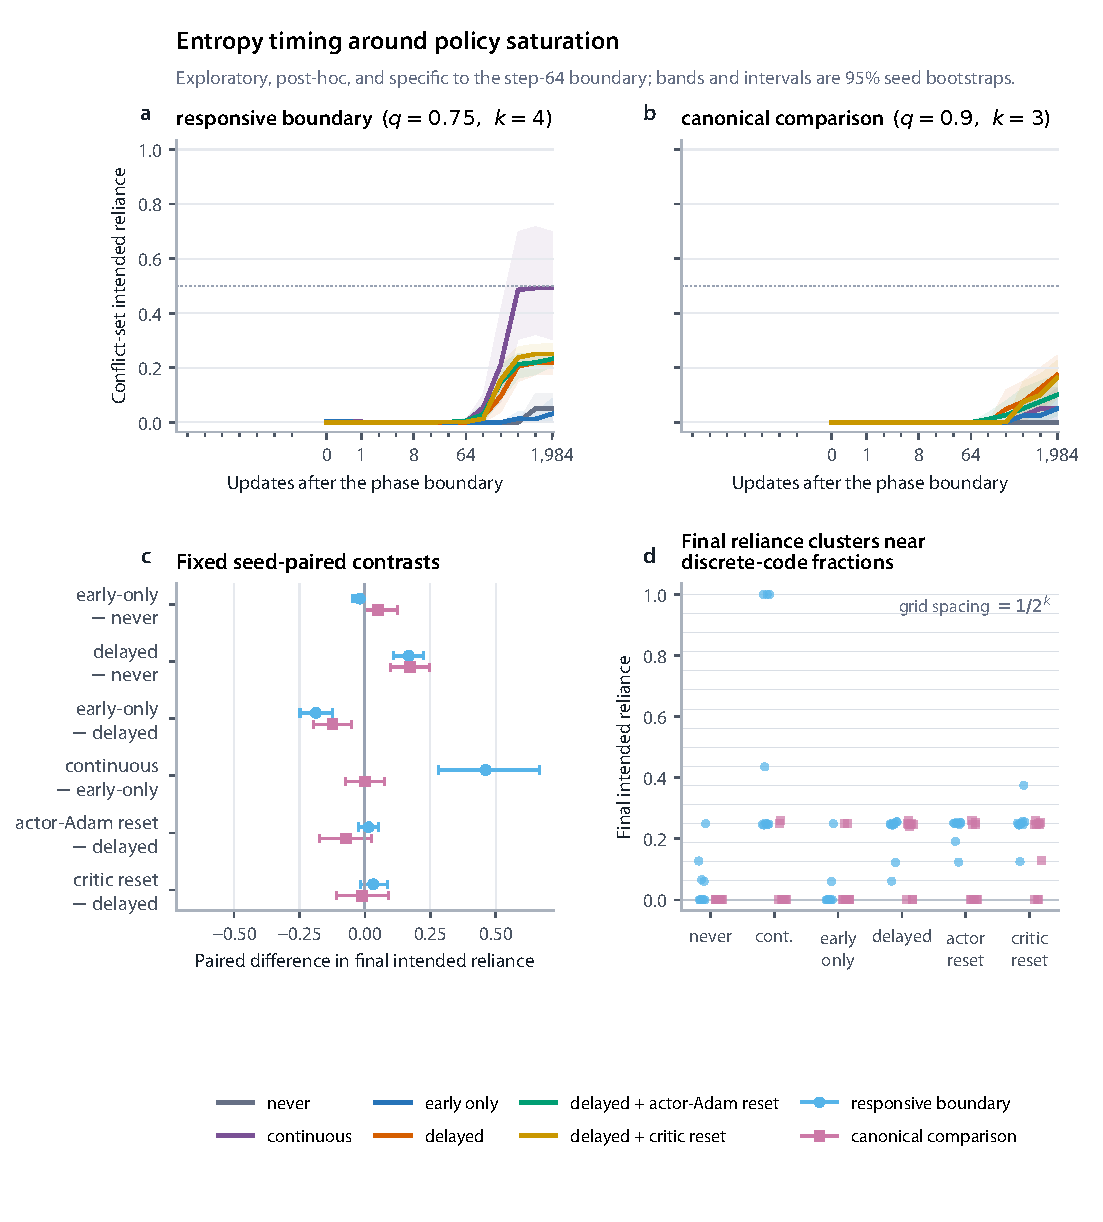
\includegraphics[width=\linewidth]{fig14_entropy_timing_exploratory.pdf}
  \caption{\textbf{Entropy can reheat a saturated policy without completing the intended rule.} \textbf{a--b}, Mean conflict-set intended reliance after the step-64 boundary for the selected responsive cell and the canonical comparison cell. The horizontal .5 line is the secondary persistent-acquisition threshold. \textbf{c}, Fixed paired endpoint contrasts; circles and squares distinguish the two cells. \textbf{d}, Individual seed endpoints cluster near fractions of the finite parity truth table rather than forming a smooth continuum. Bands and intervals are 95\% seed-bootstrap intervals. The design, cell selection, and every inference in this figure are post-hoc.}
  \label{fig:entropytiming}
\end{figure}

\begin{takeaway}
Entropy timing changes the path through a proxy trap. Late pressure can restore causal reliance after saturation, but in these cells it usually repairs only a subset of the intended truth table; sustained pressure sometimes completes the rule, in a strongly cell-dependent way. The experiment observes the behavioral change, not the underlying gradient mechanism.
\end{takeaway}

\FloatBarrier
\section*{Finding 10: Temporal structure matters, but fresh noise does not wash out}

Classical analyses show that adding small independent input noise can act like a regularizer after averaging over perturbations, while modern data-augmentation theory likewise treats perturbations as changes to the effective estimator rather than as inert errors \citep{bishop1995noise,dao2019augmentation}. Those results concern the effective training objective; they do not imply that the final policy must match one trained on clean inputs.

The usual averaging argument concerns an estimate of a fixed quantity. If independent perturbations $\epsilon_i$ have mean zero, then their sample average shrinks like
\[
\frac{1}{N}\sum_{i=1}^{N}\epsilon_i=O_p(N^{-1/2}).
\]
Our learner is not merely estimating the mean of $P+\epsilon$. It is choosing between computations: directly read a noisy proxy $P$, or learn the exact interaction $Y=\prod_i R_i$. Even zero-mean noise can reduce the proxy's margin and change which computation optimization selects. The perturbations may average to zero without the \emph{learned policy} returning to the policy trained on a clean proxy.

Persistence supplies a second distinction. Step-resampled noise changes on every contextual row. Episode-static noise is shared by four repeated choices and is then redrawn. State-static noise returns with the same semantic state. Repeated exposure can therefore reinforce a state-tied offset as part of the training context, even though the experimenter calls it noise. This motivates two separate predictions: fresh observation noise should produce less proxy reliance than state-tied noise, and its effect should contract toward the clean baseline as the amount of data grows. The complete experiment supports the first prediction and reverses the second.

\subsection*{Experiment}

We fixed $q=.9$, a degree-three intended rule, and a 5,833-parameter selector. The dense factorial crosses four algorithms, four temporal structures, three perturbation locations, five marginal scales, four recurrence counts, three dataset sizes, and ten seeds: 28,800 runs. Each model receives eight passes over $N\in\{2{,}560,10{,}240,40{,}960\}$ rows, or 20,480, 81,920, and 327,680 presentations. A separate 100-run terminal-reward panel tests a semantic equivalence control.

The primary temporal comparison uses the 7,680 positive-scale observation-noise runs. Every contrast matches algorithm, scale, recurrence, sample size, and seed before planned cells are averaged within seed. The scaling analysis adds the 1,920 scale-zero observation controls and compares every noisy model with its matched clean-proxy baseline. Label and reward perturbations are analyzed separately because they intervene on different objectives.

\subsection*{Persistent observation noise preserves proxy control}

The full three-size panel strengthens the earlier temporal result (\fig{fig:noise}a). Step minus episode is only +.0187, 95\% \CI{} $[.0145,.0231]$, entirely inside the preregistered $\pm.05$ practical-equivalence band. Episode minus state is +.0991 $[.0882,.1112]$, making the combined step-minus-state contrast +.1178 $[.1070,.1300]$. Thus most of the temporal effect appears when the perturbation becomes permanently tied to semantic state, rather than when it merely persists for four rows.

The step-minus-state contrast is positive under every learning rule: +.0941 $[.0839,.1045]$ for clean SFT, +.0841 $[.0729,.0959]$ for trajectory SFT, +.0987 $[.0894,.1087]$ for on-policy imitation, and +.1942 $[.1738,.2174]$ for RL. Positive means greater intended-goal reliance under fresh noise, so state-static perturbations leave substantially more proxy control. The causal feature intervention points the same way: the probability effect of flipping $P$ is larger after state-static training, with step minus state $=-.1572$ $[-.1743,-.1423]$. The difference is therefore not merely a hard-threshold artifact in $\rhoY$.

An exploratory recurrence split makes the structural distinction more concrete. With only one episode per semantic state, episode- and state-static noise are effectively the same construction, and episode minus state is +.0012 $[-.0061,.0083]$. The gap grows to +.0729 with four episodes, +.1646 with 16, and +.1577 with 64. It is also nonlinear in scale: step minus state is +.0444 at scale .25, +.1463 at .5, +.1656 at 1, and +.1148 at 2. At very high corruption, even state-static noise begins to dislodge the proxy.

Ordinary generalization accuracy would obscure this result. On new states drawn at the training correlation $q=.9$, state-static models have mean $\rhoY=.851$, slightly above step-noise models at .826. When the evaluation forces $P=-Y$, the ordering reverses sharply: .436 versus .554. State-static models also do not have a larger seen--new gap, so these results are not direct evidence that the network memorizes individual offsets. They establish that state-tied training corruption preserves the proxy's causal control; the internal mechanism remains unresolved.

\begin{figure}[!htbp]
  \centering
  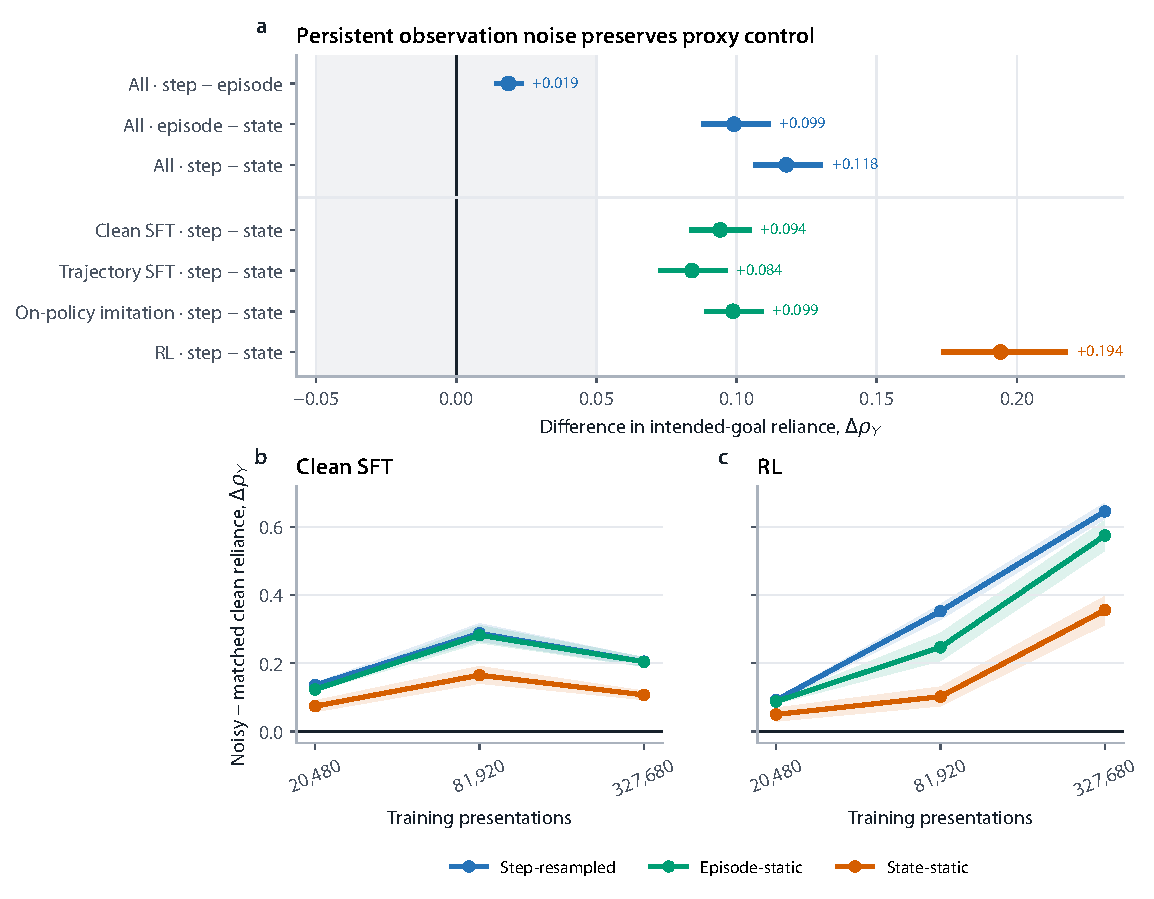
\includegraphics[width=\linewidth]{fig5_temporal_noise.pdf}
  \caption{\textbf{Temporal structure matters, while fresh noise moves behavior away from the clean baseline.} \textbf{a}, Matched positive-scale observation-noise contrasts. Positive values mean that the condition named first has greater intended-goal reliance and therefore less proxy control. The shaded region is the $\pm.05$ practical-equivalence band. \textbf{b,c}, Intended reliance under positive observation noise minus the matched scale-zero control, averaged over noise scales and recurrence counts within each seed. Bands are 95\% seed-bootstrap intervals. Fresh noise remains behaviorally consequential at the largest sample size; the effect is especially large for RL.}
  \label{fig:noise}
\end{figure}

\subsection*{More data amplifies fresh noise's effect instead of restoring clean behavior}

To test averaging, define the matched behavioral gap
\[
g(N)=\rhoY(\text{positive noise},N)-\rhoY(\text{scale zero},N).
\]
For each seed, scale, recurrence level, and algorithm, we fit the slope of both $g(N)$ and $-|g(N)|$ against $\log_2$ presentations. The first statistic records direction: a positive slope means the noisy model becomes more intended-goal-reliant relative to its clean control. The second records recovery: a positive slope means the absolute gap contracts toward zero.

Fresh noise moves in the intended direction, but it does not recover to clean behavior. Pooled over algorithms and planned strata, the signed step-noise slope is +.0443 intended-reliance points per doubling $[.0411,.0475]$, while the gap-to-zero slope is $-.0441$ $[-.0472,-.0410]$. Clean SFT shows the same reversal, with slopes +.0171 $[.0132,.0212]$ and $-.0171$ $[-.0208,-.0134]$. Its average gap rises from .136 to .287 and then falls to .204 across the three sample sizes, so the effect is not monotone even though the registered log-linear slope is positive. RL is unambiguous: its fresh-noise gap rises from .091 to .352 to .646, yielding signed and recovery slopes of +.1386 $[.1331,.1444]$ and $-.1383$ $[-.1436,-.1334]$ (\fig{fig:noise}b,c).

The same result appears in the comparison with state-static noise. The fresh-minus-state signed-gap slope is +.0211 $[.0175,.0250]$: fresh noise increasingly favors the intended rule relative to state noise. But its gap-contraction advantage is $-.0207$ $[-.0250,-.0167]$, the opposite of recovery. All four algorithms show this pattern. The registered combined decision is therefore evidence against the sample-averaging claim, even though the temporal ordering itself is supported.

This does not violate the law of large numbers. The clean baseline at $q=.9$ is itself attracted to the proxy, especially under RL. Fresh noise weakens that easy channel; with more rows and, under the fixed-eight-epoch protocol, more optimizer updates, the harder exact rule can win. Returning to the clean baseline would mean returning toward proxy control. The result distinguishes cancellation of a random variable from reversal of a path-dependent learning decision.

\subsection*{The effect depends on where noise enters}

The large temporal effect is specific to perturbing the observed proxy. For label noise across the three imitation methods, step minus state is +.0279 $[.0210,.0351]$; for dense reward noise under RL it is $-.0336$ $[-.0416,-.0251]$. Both intervals lie inside the $\pm.05$ practical-equivalence region. In the terminal-reward control, step- and episode-static reward noise are the same intervention because only one reward is emitted per episode. Their matched difference is $-.0029$ $[-.0053,-.0004]$, also practically equivalent. Finally, all 9,600 objective-ignored cells are exactly invariant across their nominal noise settings. These controls argue against treating ``temporal noise'' as one location-independent mechanism.

\begin{takeaway}
Matching marginal variance is not enough to predict a perturbation's effect on learned goal control. Persistence matters when noise corrupts the proxy observation, but independent zero-mean noise need not become behaviorally irrelevant: by weakening a competing proxy, it can permanently change which rule training selects.
\end{takeaway}

\section*{Finding 11: Counterevidence suppresses an old proxy faster than making it unavailable---but perfect reversal can train the inverse proxy}

Once a proxy controls behavior, there are several ways to stop rewarding it. We can remove it from the input, show examples on which it is unrelated to the target, or make it systematically wrong. These interventions differ in the gradient they supply. Removal prevents further use of the feature but gives its direct pathway no feature-specific corrective signal. Decorrelation repeatedly varies the feature while making it useless. Reversal supplies an even stronger gradient against the old positive mapping.

This is related to, but narrower than, catastrophic forgetting in sequential learning: later training changes weights that supported earlier behavior \citep{kirkpatrick2017forgetting}. Our question is not simply whether performance on an old task falls. We ask whether the old proxy still controls decisions when it is restored, and we intervene separately on the proxy and exact-code channels. That distinction becomes essential in the perfectly reversed condition.

\subsection*{Installing, suppressing, and restoring a proxy}

We first train until reliance on $P$ exceeds .9 at three consecutive evaluations. All 1,920 runs pass this installation gate. We then train for 1,024 further updates under one of four interventions: remove $P$; decorrelate it from $Y$; reverse it so that $q_B\in\{.40,.25,.10,0\}$; or decorrelate it while adding a new 99\%-accurate proxy. The primary 840 runs cross three installation accuracies and four widths; 1,080 separately labeled runs repeat selected arms with weight decay.

During the second phase we evaluate every update on a fixed restoration probe where the original proxy is present and conflicts with $Y$. Its behavioral half-life is the first time old-sign proxy reliance falls halfway from its installed level toward zero. Decorrelation halves old behavior 49.37 updates sooner than removal, 95\% \CI{} $[-85.73,-22.57]$. Every one of the 120 matched seed--installation--width cells has this sign. Reversal is faster again: relative to decorrelation, the matched differences range from $-17.71$ updates at $q_B=.40$ to $-23.61$ under perfect reversal, and all 480 matched cells have the reversal-first ordering (\fig{fig:unlearning}a).

At the end of training, restoration exposes a residual that current-distribution performance hides. All removal, decorrelation, and reversal models are perfect on the visible second-phase distribution. Restoring the absent proxy reduces removal-arm intended accuracy to .9462, however, versus .9958 after decorrelation. Mean restored old-proxy reliance is .0538 after removal and .0042 after decorrelation; their paired difference is $-.0496$ $[-.0705,-.0294]$. The removal distribution is highly heterogeneous: 90 of 120 runs have no residual proxy-following, while one small model remains near chance at $\rhoP=.499$ (\fig{fig:unlearning}b).

\begin{figure}[!htbp]
  \centering
  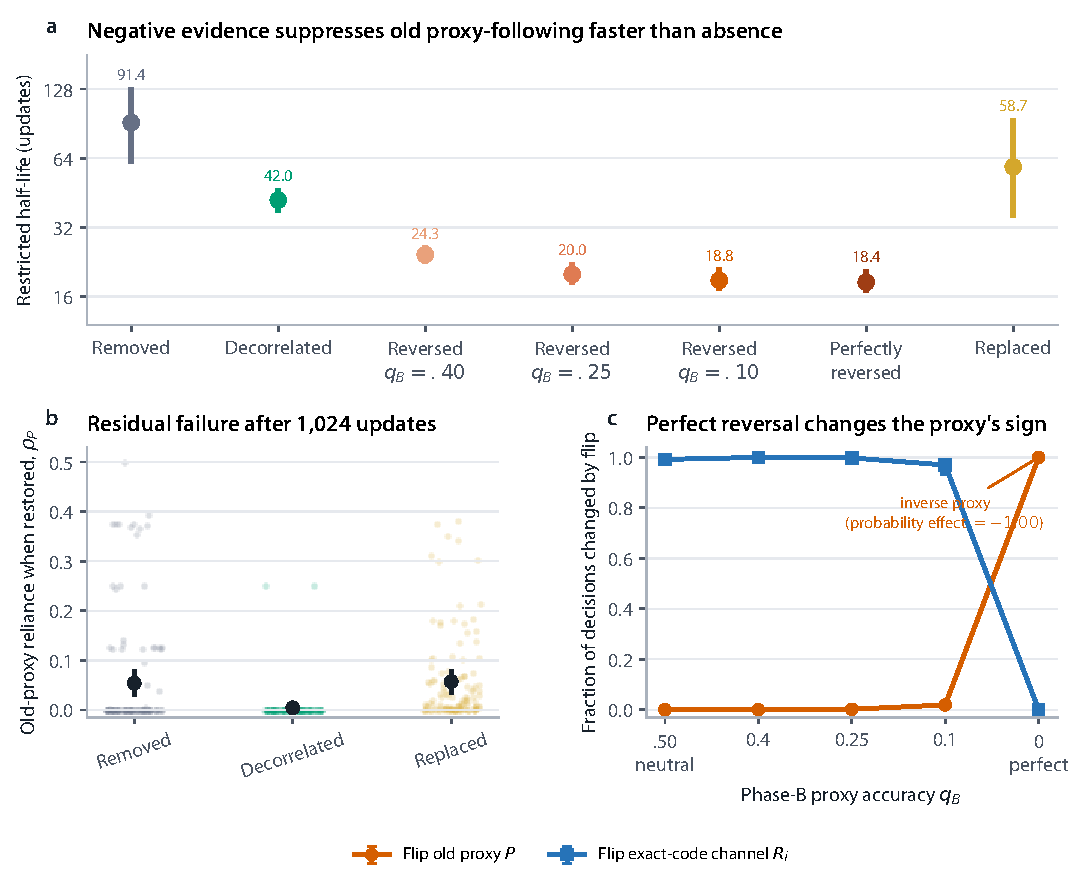
\includegraphics[width=\linewidth]{fig6_unlearning.pdf}
  \caption{\textbf{Negative evidence changes old behavior faster than absence, but behavior alone can misidentify what replaced it.} \textbf{a}, Restricted mean half-life of old-sign proxy-following; intervals bootstrap ten seed-level aggregates. One removal run is right-censored at 1,024 and retained at the horizon. \textbf{b}, Seed-cell outcomes after restoring the old proxy. Colored points are individual runs; black points and bars are seed-aggregated means and 95\% intervals. Replacement leaves widespread small residuals, while removal produces rarer large failures. \textbf{c}, Hard decision changes after flipping the old proxy or one exact-code channel. Imperfect reversal transfers causal control to the exact rule. Under perfect reversal, flipping $P$ flips every decision and flipping $R_i$ changes none: the model uses $-P$, not the exact code.}
  \label{fig:unlearning}
\end{figure}

\subsection*{Perfect behavioral recovery can still be proxy control}

The restoration probe creates a subtle identification problem under perfect reversal. There, every second-phase example satisfies $P=-Y$. Both ``compute $Y$ from the exact code'' and ``output $-P$'' achieve zero loss, and both appear perfectly intended-goal-reliant on the restoration set. The causal flips separate them. At $q_B=0$, flipping $P$ flips 100\% of decisions and changes intended-action probability by $-.9997$, while flipping an $R_i$ changes no decisions. The model has learned the inverse proxy (\fig{fig:unlearning}c).

The nearby reversal arms behave differently because rare exceptions distinguish $-P$ from $Y$. At $q_B=.10$, flipping $P$ changes 1.90\% of final decisions while flipping an $R_i$ changes 96.97\%. At $.25$ and $.40$, causal dependence on $P$ is smaller still. Their trajectories initially move toward the inverse shortcut and then leave it as counterexamples accumulate. Thus the behavioral half-life measures loss of the \emph{old sign} of proxy-following; it does not, by itself, measure erasure of proxy dependence.

The weight-decay sensitivity does not materially change this result. Across $10^{-5}$ to $10^{-3}$, removal's mean restored reliance changes from .0538 to at most .0539 and its half-life remains about 91 updates. Over only 1,024 AdamW steps these settings directly shrink parameters very little, so the null result does not exclude stronger regularization or explicit unlearning methods.

\begin{takeaway}
Evidence that contradicts a shortcut suppresses its old behavior faster than simply making it unavailable. But a reversal test needs additional disagreements: if the inverse shortcut is itself perfect, apparently correct behavior can still be completely proxy-controlled.
\end{takeaway}

\section*{Finding 12: A replacement shortcut restores performance before it removes the old failure}

Replacing one shortcut with another can make a system look repaired without creating much pressure to learn the intended computation. If the new route removes almost all residual loss immediately, gradients supporting the exact rule become small. The model can then reach excellent current-distribution performance while old behavior decays only gradually. This is a sequential version of the competition and gradient-starvation pattern seen in the earlier acquisition experiments.

The replacement arm decorrelates the old $P$ exactly as the neutral arm does, but adds a new proxy $P_{\mathrm{new}}$ with 99\% accuracy. This makes it a useful comparison: both arms contain the same direct evidence that the old proxy is useless, while only one offers a cheap alternative.

On the replacement distribution, models reach .9990 target accuracy and .9910 agreement with $P_{\mathrm{new}}$. An exploratory three-checkpoint mastery criterion is reached after 18.3 updates on average, while old-sign behavior takes 58.7 updates to halve. Current performance precedes that half-life in all 120 runs. When the new proxy is removed and the old one restored, intended accuracy falls to .9430 and old-proxy-like reliance is .0570---essentially the same mean residual as removal and far above decorrelation's .0042 (\fig{fig:unlearning}b).

The distribution distinguishes replacement from removal more clearly than the means. Residual behavior is nonzero in 103 of 120 replacement runs but only 30 of 120 removal runs: replacement produces many small failures, while absence produces fewer, sometimes much larger ones. The normalized area under the old-reliance trajectory is .2483 after replacement, .1147 after removal, and .0411 after decorrelation. Replacement minus decorrelation is +.2073 $[.1885,.2244]$.

Agreement with the new proxy is not exclusive causal control, because $P_{\mathrm{new}}$ and $Y$ usually agree. Flipping it changes 9.60\% of decisions and changes intended-action probability by $-.1379$; the model uses it partly, while also building some exact-rule behavior. The resulting trajectory includes an interference plateau rather than persistence of one fixed rule: restored old reliance falls, rises slightly around updates 128--256, and then declines.

\begin{takeaway}
Validation performance can recover much earlier than an old failure disappears. Introducing a new high-accuracy shortcut may reduce the optimization pressure that would otherwise consolidate the intended rule.
\end{takeaway}

\section*{Finding 13: Old-goal training raises alignment cost, but does not explain rebound}

A model that returns to an earlier behavior after later fine-tuning may have retained that behavior in a dormant form. But the same observation has a simpler alternative explanation: the new data may once again underidentify the goal, allowing any model to reacquire the easy rule. Recent language-model work reports ``elasticity,'' in which post-alignment models return toward their pretraining behavior and the effect grows with model and pretraining scale \citep{ji2025alignment}. To interpret such rebound as memory, the decisive comparison is not rebound versus zero; it is rebound versus a model that received the same later training without the relevant history.

\subsection*{Separating history from renewed shortcut learning}

We compare three histories. The old-history model first receives $N_0\in\{512,2{,}048,8{,}192,32{,}768\}$ examples labeled by the old proxy. A compute-matched sham receives the same number of updates on balanced random labels, and a no-history control skips this stage. All models are then trained toward the intended goal. The fixed-volume design gives exactly 8,192 intended-goal examples; the behavior-matched design trains until intended reliance remains in the narrow .90--.93 band for two evaluations. Four final perturbations range from goal-unidentifying agreement data to partial old-goal evidence.

The behavior-matched comparison equalizes visible pre-perturbation behavior: old-proxy reliance is .081 for both old and sham histories and .080 for the no-history control. Yet all three return to essentially the same behavior afterward (\fig{fig:hysteresis}a). Neutral agreement data and data with the intended channels removed take final old-goal reliance to exactly 1.000 in every group. With old-goal labels on 75\% of disagreement cases, the three outcomes are approximately $.968,.962,.967$; with only 55\%, they are $.662,.651,.656$.

The matched old-minus-sham rebound contrasts are consequently small. Averaged within seed over capacity and available $N_0$ cells, they are +.0010 $[-.0003,+.0024]$ for neutral data, the same for intended-signal removal, +.0047 $[+.0025,+.0068]$ for the 75\% arm, and +.0085 $[+.0030,+.0140]$ for the 55\% arm. Every interval is far inside the preregistered five-point practical margin. The large raw rebound therefore does not identify dormant history: ambiguous retraining returns even scratch and sham models to the one-coordinate proxy.

\begin{figure}[!htbp]
  \centering
  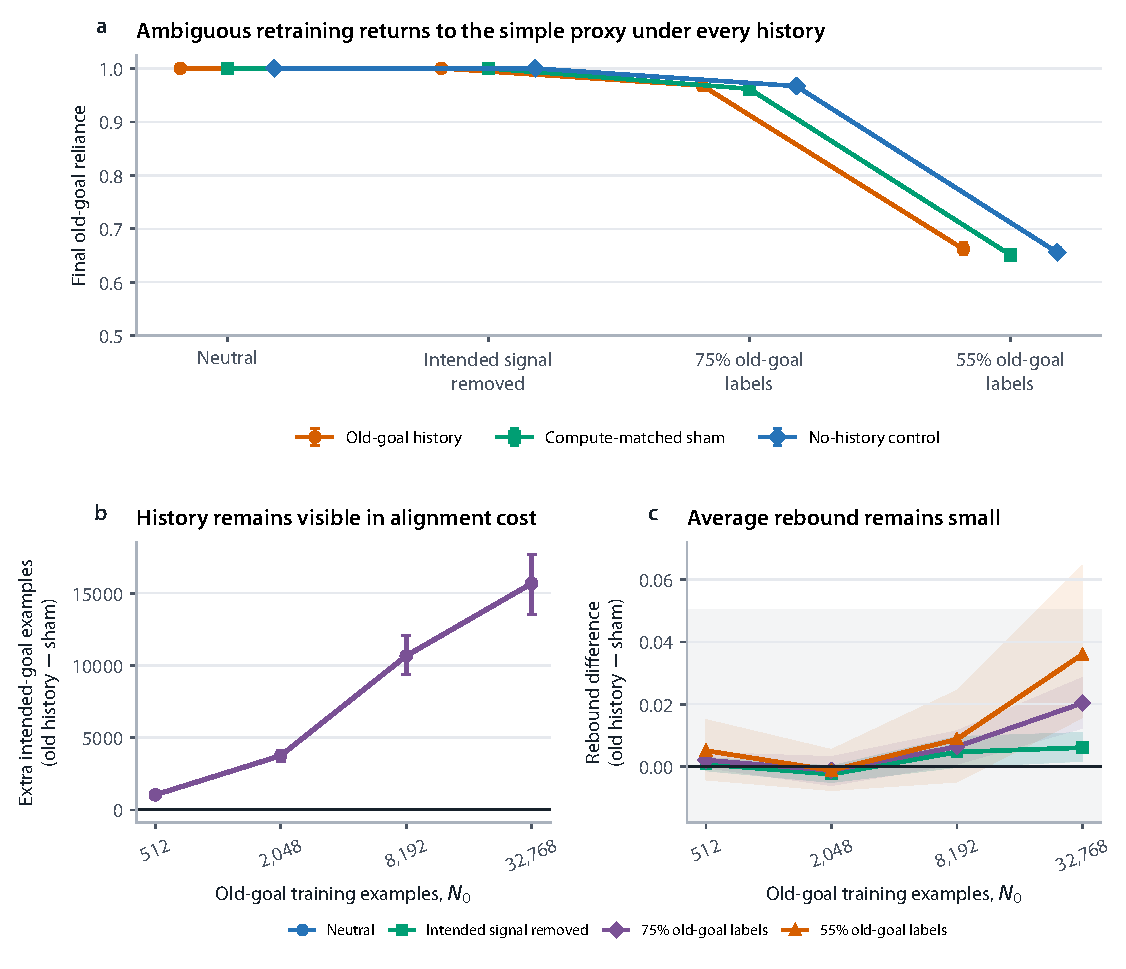
\includegraphics[width=\linewidth]{fig7_hysteresis.pdf}
  \caption{\textbf{History affects alignment cost much more than final rebound.} \textbf{a}, Final old-goal reliance in the behavior-matched design. The old-history, compute-matched-sham, and no-history curves nearly overlap. \textbf{b}, Additional intended-goal examples required to place an old-history model in the same .90--.93 behavior band as its matched sham. \textbf{c}, Matched old-minus-sham rebound by old-goal training volume. The shaded strip is the $\pm.05$ practical-equivalence region. Intervals bootstrap seeds after available width cells are averaged within seed; the highest-volume comparison contains eight seeds.}
  \label{fig:hysteresis}
\end{figure}

\subsection*{History remains measurable in the cost of realignment}

Although final rebound is not history-specific on average, the path to matched behavior is. Relative to its compute-matched sham, an old-history model needs 1,046 additional intended-goal examples after $N_0=512$, with 95\% \CI{} $[888,1{,}204]$. The excess grows to 3,758 $[3{,}342,4{,}125]$, 10,667 $[9{,}292,12{,}042]$, and 15,677 $[13{,}479,17{,}750]$ as $N_0$ rises (\fig{fig:hysteresis}b). Prior training therefore leaves a real historical scar, but it is more evident in replacement cost than in the eventual rebound endpoint.

The highest-volume behavior-matched slice also shows a small conditional rebound advantage for old history: +.0061 under neutral/removal, +.0204 with 75\% old-goal labels, and +.0360 with 55\%. These estimates use only 11 matched width--seed cells across eight seeds and contain no width-128 pair, so they are secondary rather than a clean capacity effect (\fig{fig:hysteresis}c).

Eligibility limits the scaling interpretation. Only 479 of 720 distinct pre-perturbation cells enter the primary comparisons. In the behavior-matched design, 150 cells overshoot the narrow .90--.93 band and only one fails to reach .90; width 128 contributes just six of 90 eligible cells. In the fixed-volume old-history arm, greater $N_0$ is strongly coupled to which widths can realign successfully. The preregistered correlations---larger models and histories reactivate faster but show less change-score rebound---are therefore descriptive and selection-sensitive. Larger sham and no-history models also reacquire the proxy faster, so speed is not specific evidence of memory.

\begin{takeaway}
Rebound is not a memory assay unless it is compared with scratch and compute-matched histories. Here prior goal training clearly increases the data needed for realignment, while ambiguous later data makes nearly every model reacquire the simple proxy.
\end{takeaway}

\section*{Finding 14: More capacity makes a context-gated repertoire reliable, but learning the rules is cheaper than learning the gate}

A model need not settle on one globally useful proxy. If it can represent two rules and a context-dependent interaction, its behavior may be better described as a repertoire plus a selector. The selector is an additional learned computation: showing that an architecture can learn either rule separately does not show that optimization can compose both and invoke the right one. This resembles gating in mixture-of-experts models, where an input-dependent gate determines which expert controls the output \citep{makkuva2020gated}.

\subsection*{Two goals and one selector}

We generate two independent binary goals $P_0$ and $P_1$. A latent environment $E$ selects the rewarded one, so $Y=P_E$, and the observed context is $C=E$ during training. A policy that always follows one proxy is correct on
\[
\tfrac12(1)+\tfrac12(\tfrac12)=.75
\]
of examples; following $P_C$ is perfect. For every architecture or update budget, separate calibration models test whether $P_0$ and $P_1$ can each be learned alone. The main policy is judged on strict switching: on rows where $P_0\ne P_1$, clamping the same input to $C=0$ must produce $P_0$ and clamping it to $C=1$ must produce $P_1$.

The architecture sweep crosses three depths, seven widths, and ten seeds. Tiny networks show a seed-sensitive transition rather than a smooth compromise (\fig{fig:multiplicity}a,b). At depth 1, width 2, all ten single-rule controls pass, but only five selectors cross .9; five seeds are perfect or nearly perfect, four have almost no gate, and one implements roughly one branch. Mean strict switching .558 is therefore not typical of most individual runs. Width 4 raises selector success to nine of ten, and width 8 to ten of ten. Depth is not interchangeable with width: a 105-parameter depth-2 network succeeds in ten of ten seeds, while a 145-parameter depth-4 network has two calibration failures and only seven selector successes.

After calibration failures are excluded, the planned within-seed association between total parameters and strict switching is positive, Spearman $\rho=.428$ $[.345,.502]$. Only seven seeds contribute because three are perfect at every eligible architecture, leaving their rank correlation undefined. We interpret this as capacity increasing the reliability with which optimization finds a conditional solution, not as a representational threshold: some 85-parameter networks already switch perfectly.

\begin{figure}[!htbp]
  \centering
  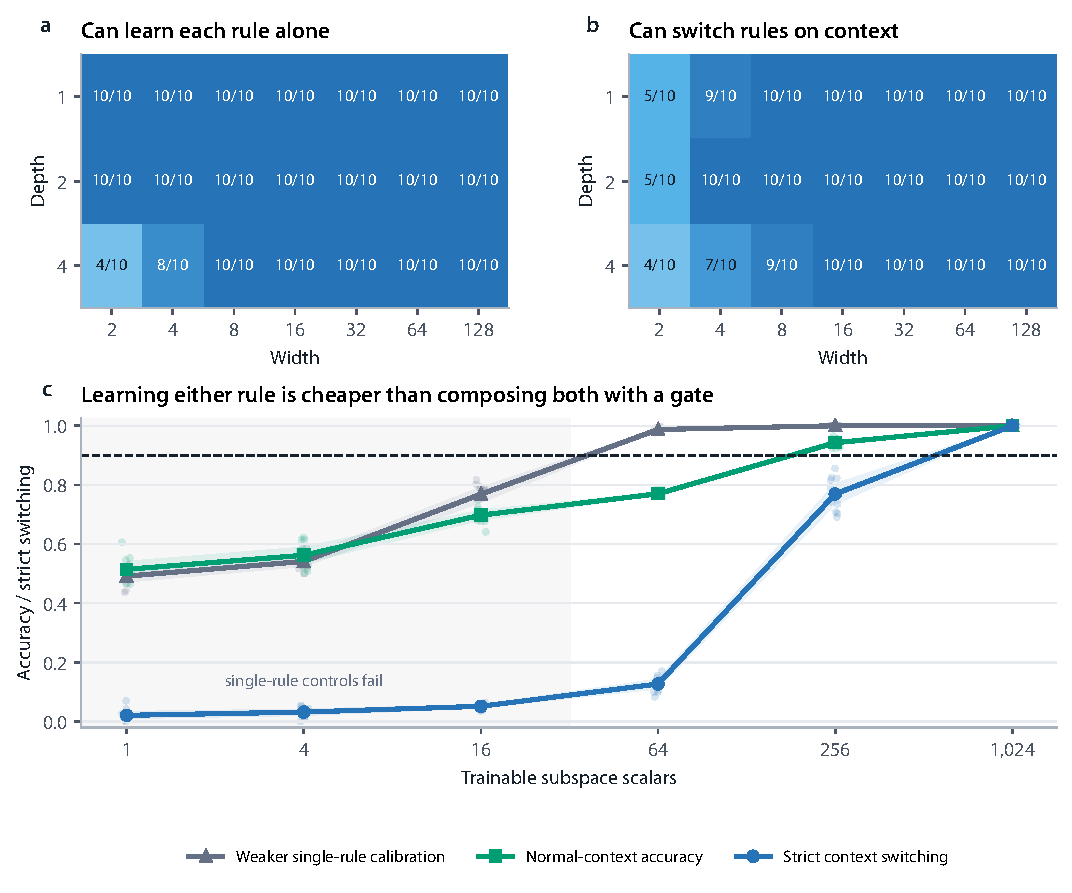
\includegraphics[width=\linewidth]{fig8_multiplicity_capacity.pdf}
  \caption{\textbf{Learning the candidate rules and learning their selector have different costs.} \textbf{a--b}, Fraction of ten seeds that master both single-rule calibrations or the context selector at each full-update architecture. Showing counts avoids hiding the multimodal small-model transition behind a mean. \textbf{c}, A fixed 52,225-parameter residual model trained through random parameter subspaces. Dots are individual seeds and lines are seed means. At 64 scalars both rules are individually accessible, but strict switching remains .127; perfect switching appears only at 1,024. The dashed line is the .9 success threshold.}
  \label{fig:multiplicity}
\end{figure}

\subsection*{Learning either rule is much cheaper than learning when to use it}

The update-capacity sweep fixes a 52,225-parameter residual model and trains it through random subspaces of 1 to 1,024 scalars. At 64 scalars, the weaker single-rule calibration averages .987 and all ten calibration pairs pass, yet normal task accuracy is only .770 and strict switching is .127 $[.110,.143]$. At 256, both rules are individually perfect and normal accuracy reaches .943 $[.934,.952]$, but strict switching is .769 $[.735,.804]$ and no seed crosses the .9 selector criterion. Only 1,024 yields perfect switching in all ten seeds (\fig{fig:multiplicity}c).

The first tested selector-mastering budget is therefore 16 times the first budget that masters both rules separately. These count-sketch subspaces change geometry as well as dimension, so 16 is a grid ratio rather than a lower bound on a modular selector's parameter count. The robust conclusion is comparative: access to both behaviors does not imply access to their composition.

\subsection*{The context cue causally controls which goal is used}

At the highest model and update capacities, clamping $C=0$ makes flipping $P_0$ flip every decision and flipping $P_1$ flip none. Clamping $C=1$ reverses this matrix exactly (\fig{fig:context}b). This representation-free intervention establishes conditional causal control, although it does not prove that the network contains cleanly separable ``goal modules''; a monolithic Boolean circuit could implement the same behavior.

Reliable context use also creates a predictable vulnerability. As update capacity grows from 64 to 1,024, normal accuracy rises from .770 to 1.000, while accuracy under a context cue forced opposite to the latent environment falls from .729 to .500. At maximum capacity the model follows the observed-context goal perfectly even when that cue is wrong (\fig{fig:context}a). The latent environment is not an input, so this does not show the model ignoring an observable reward variable; it shows that training made $C$ authoritative.

Removing or randomizing context returns accuracy to .750 and .7516, respectively, the one-rule ceiling. In the removed condition the model defaults to $P_0$. This fallback should not be read as historical or simplicity bias: removal is encoded as $C=0,C_{\mathrm{present}}=0$, while the presence bit was always one during training, so missingness is structurally aliased with the zero-coded branch.

\begin{figure}[!htbp]
  \centering
  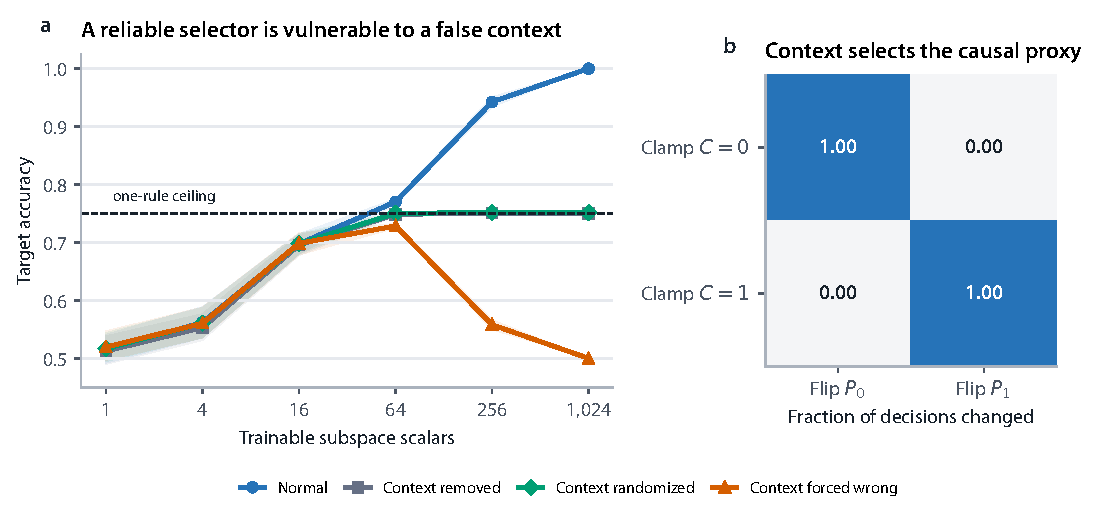
\includegraphics[width=\linewidth]{fig9_context_control.pdf}
  \caption{\textbf{A learned context gate is both causal and manipulable.} \textbf{a}, Accuracy across context interventions in the update-capacity sweep. The dashed .75 line is the expected accuracy of always following one proxy. As the selector improves, a forced-wrong context becomes more damaging. \textbf{b}, Hard decision-flip rates at the 1,024-scalar budget. Only the proxy selected by the clamped context has causal control.}
  \label{fig:context}
\end{figure}

\begin{takeaway}
A model can retain multiple candidate goals behind a learned selector. Audits should therefore test not only which behaviors are available, but which contextual variables gate them---including interventions that make the selector confidently choose the wrong branch.
\end{takeaway}

\section*{Finding 15: More than a third of policies do not match a pure-goal signature---and most fail the tested fixed three-way mixture}

The baseline conflict set makes attribution deceptively easy: when $P=-Y$, every binary action agrees with exactly one candidate. Real systems can contain several partially reliable shortcuts at once. A learner need not commit globally to one of them. It can weight them, follow different candidates in different regions, or learn another rule not included in the analyst's menu. In that setting, asking only ``which goal won?'' can force conditional or simply misspecified behavior into a false single label.

We therefore study three simultaneously available rules. A direct proxy $P$ has accuracy $q_P\in\{.9,.99\}$. A second proxy $Q$ has accuracy $q_Q\in\{.9,.95,.99\}$ but is encoded as degree-two or degree-three parity. The intended rule $Y$ is always correct and encoded as degree-three or degree-five parity. Width is 16 or 64, and every candidate is separately calibrated before competition. All three standalone decoders reach 1.000 accuracy in all 960 runs, so later differences concern selection under competition rather than terminal representability.

\subsection*{Three disagreements identify three candidate signatures}

No single conflict panel can distinguish these rules. We instead evaluate the same trained policy where both proxies are wrong, only $P$ is wrong, and only $Q$ is wrong. A pure $P$ policy has target-accuracy signature $(0,0,1)$ across those panels; pure $Q$ gives $(0,1,0)$; and pure $Y$ gives $(1,1,1)$. We pair these diagnostics with interventions that flip $P$, an active $Q$ channel, or an active $Y$ channel on the same inputs.

A run receives a pure-goal label only if every diagnostic panel lies within .10 of one candidate's signature, that candidate has the largest causal effect, and its mean hard-flip influence is at least .5. This is intentionally conservative. The nearest diagnostic signature and largest causal influence agree in 929 of 960 runs, but only 607 satisfy the full pure-selection rule. The remaining 353 policies are behaviorally mixed or unresolved. Under independent proxy errors, non-pure behavior is the majority: 259 of 480 runs.

In a post-hoc model check, a simple static mixture makes a stronger, testable prediction. If $A_{--}$ is target accuracy when both proxies are wrong, $A_{P-}$ when only $P$ is wrong, and $A_{Q-}$ when only $Q$ is wrong, its implied weights are
\[
w_Y=A_{--},\qquad w_Q=A_{P-}-A_{--},\qquad w_P=A_{Q-}-A_{--},
\]
and they should be nonnegative and sum to one. Allowing a .05 margin on weights and closure, 71.8\% $([70.1,73.4]\%)$ of runs are behaviorally compatible with this model, but the aggregate is dominated by pure one-hot policies: 587 of the 607 pure-signature runs are compatible. Only 102 of the 353 non-pure runs are compatible, or 28.9\% $([26.2,31.6]\%)$ conditional on being non-pure. Thus only 10.6\% $([9.4,12.2]\%)$ of the full grid is both non-pure and consistent with the fixed three-way mixture. The mean absolute closure error is .127 $([.118,.134])$. Incompatible cases could reflect panel-dependent interactions, an unmodeled rule, or another violation of the three-candidate mixture; the panels do not distinguish these explanations. None of this inversion identifies literal latent components inside the network.

\subsection*{Some apparent mixtures are conditional rules fitted to missing support}

A later adaptive continuation resolves one recurring non-pure endpoint. Thirty of its 240 models have the same thresholded truth-table signature: use $Y$ when $P=Q$, and use $Q$ when they disagree. Every occurrence is in a nested-error cell with $q_Q>q_P$. In these cells, $Q$ is correct whenever the proxies disagree, while $Y$ is needed when both are wrong. The conditional rule is therefore correct on every candidate tuple that training supplies, even though it matches no pure candidate and violates the fixed-mixture equations.

The exhaustive factorial evaluation includes the two $Q$-only-error tuples that nesting removes from training. On the 30 endpoints, mean accuracy is .998 on supported tuples but only .172 on this absent case. Twenty-six also meet the stricter .9 consistency criterion across raw codewords. This does not show that every unresolved policy has a comparably compact description. It does show why ``not pure'' and ``not an additive mixture'' are negative diagnoses rather than a complete taxonomy: an underidentified training distribution can support a simple conditional extension that neither label anticipates.

\subsection*{Accuracy and accessibility trade control continuously}

Ordinary IID accuracy averages .992 $([.991,.993])$ across the grid, while the three diagnostic accuracies average .498, .724, and .803. Normalizing each candidate's hard-flip influence across the diagnostic panels assigns mean causal shares of .312 to direct $P$, .194 to encoded $Q$, and .494 to exact $Y$. These are summaries of behavioral influence, not claims that the network literally stores three scalar weights.

The shares move in the expected directions without collapsing to a universal simplicity ranking (\fig{fig:threegoals}c). Raising $q_P$ from .9 to .99 increases $P$'s share by .416 $([.402,.431])$ and reduces $Y$'s by .237 $([.209,.270])$. Raising $q_Q$ from .9 to .99 increases the encoded proxy's share by .313 $([.301,.326])$ and reduces $Y$'s by .281 $([.267,.294])$. When the two fidelities are equal, the direct proxy still receives more than twice the causal share of the parity-coded proxy (.276 versus .122), consistent with an accessibility advantage. When $Q$ is more accurate, however, its share rises to .394 while $P$ falls to .114: fidelity can overcome the direct feature's head start.

Changing the intended degree produces the largest factorial contrast observed in the registered grid. Increasing it from three to five lowers intended causal share by .584 $([.559,.607])$, while $P$ and $Q$ gain .386 and .198. Increasing the encoded proxy's degree from two to three instead shifts .109 $([.082,.138])$ toward the intended rule, and width 64 shifts .075 $([.040,.107])$ toward it relative to width 16. Goal control therefore forms a frontier among evidence quality, accessibility, and capacity. A single ``simplest goal wins'' ordering misses both the graded tradeoff and the large set of policies that cannot be described as pure selectors.

\begin{figure}[!htbp]
  \centering
  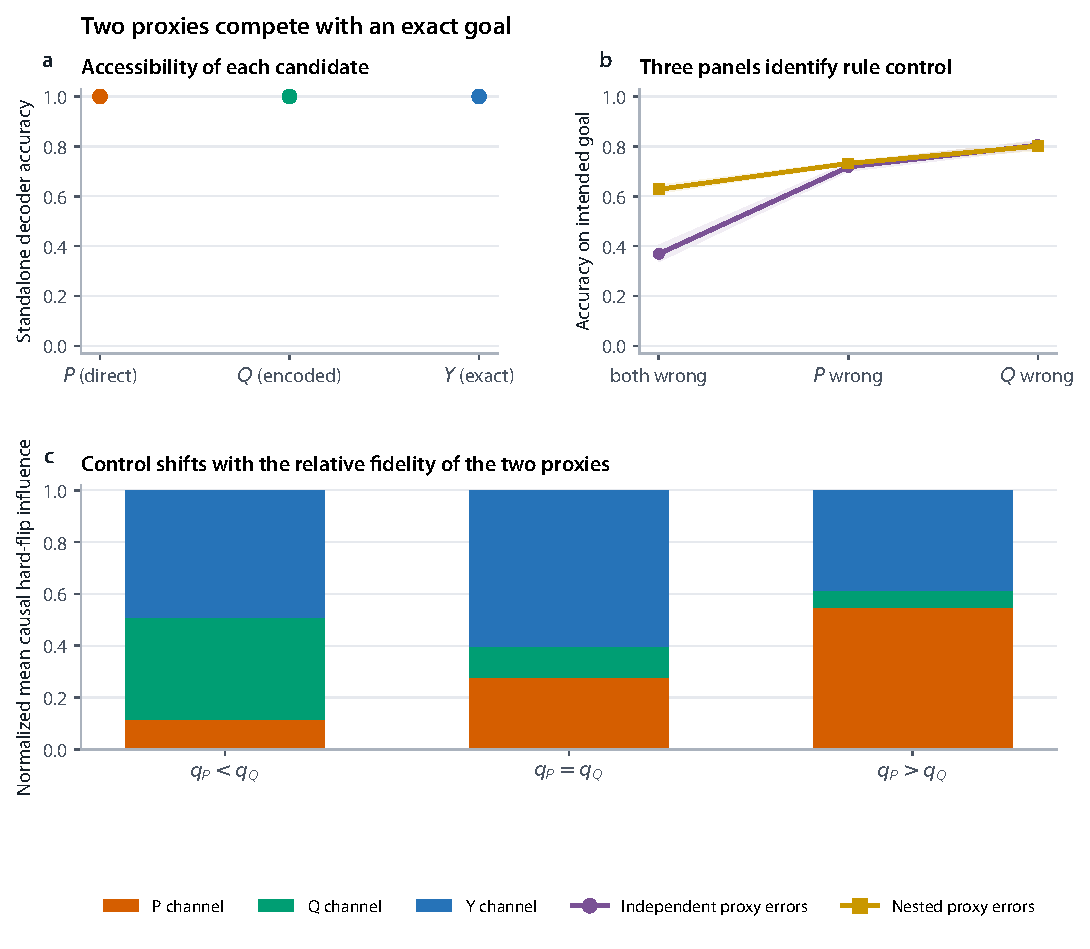
\includegraphics[width=\linewidth]{fig12_competing_goals_followup.pdf}
  \caption{\textbf{Three accessible goals produce graded and sometimes conditional control.} \textbf{a}, Each candidate decodes perfectly in isolation. \textbf{b}, Accuracy on the three diagnostic panels, split by independent versus nested proxy errors. \textbf{c}, Normalized hard-flip influence shifts toward the more accurate proxy, while the exact rule retains substantial control. Markers and bars are means after the other registered factors are averaged within seed; intervals in \textbf{a} and \textbf{b} are 95\% seed-bootstrap intervals, while \textbf{c} shows point estimates.}
  \label{fig:threegoals}
\end{figure}

\begin{takeaway}
When several plausible goals are present, a trained policy need not match any one candidate globally. Disagreement panels and causal interventions can reject a pure winner, but additional tests are needed before interpreting the remainder as a stable mixture of the named goals.
\end{takeaway}

\section*{Finding 16: Overlapping proxy failures can identify the intended rule better than more numerous isolated failures}

The earlier diversity experiment showed why many copies of one counterexample can be less useful than varied failures. With multiple proxies, there is another dimension to evidence: whether a training example rules out one alternative explanation or all of them together. An example where $P$ fails but $Q$ succeeds still has a simple explanation available. An example where both fail and only $Y$ is correct is rarer but logically sharper.

To isolate this distinction, the three-goal grid holds each proxy's accuracy exactly fixed while changing only the overlap of its error rows. In the independent arm, the two error indicators have essentially zero correlation. In the nested arm, the smaller error set is placed entirely inside the larger one. Averaged over the registered accuracy combinations, independence produces 1,054 union-error rows per 10,000, of which 29 are joint failures. Nesting produces only 767 union-error rows, of which 317 are joint failures.

\subsection*{Joint contradictions outweigh a smaller union of counterexamples}

Nesting raises accuracy on the both-wrong panel by .259 $([.232,.286])$ relative to the matched independent arm. It also raises the intended rule's normalized causal share by .113 $([.095,.133])$, primarily by reducing the encoded proxy's share by .097; IID accuracy rises by only .0046. Because the marginal accuracies, architectures, rules, sample size, and optimizer exposure are paired, this is the matched effect of changing error-overlap geometry within this design.

The benefit depends on whether the intended rule is accessible enough to use the sharper evidence. With degree-three $Y$, intended causal share rises descriptively from .672 under independent errors to .900 under nesting, and 201 of 240 nested runs become pure-$Y$ selectors. With degree-five $Y$, the corresponding shares are .203 and .200: the extra joint contradictions do not overcome the harder computation. Nesting instead makes the winning proxy more decisive, raising the rate of pure proxy selection and reducing ambiguous mixtures.

This result does not overturn the value of diverse counterexamples. The two experiments vary different objects. When the candidate set is fixed to one proxy and one intended rule, varied failures can reveal a transferable pattern. When two proxies compete, error overlap changes the number of examples on which the intended rule is the \emph{only} remaining explanation. Evidence quality depends on which hypotheses a counterexample eliminates, not simply on how many distinct rows fall outside the training correlation.

\begin{takeaway}
For several competing shortcuts, count not only how often each one fails but how their failures intersect. A smaller set of jointly diagnostic counterexamples can matter more than a larger union that always leaves some shortcut correct.
\end{takeaway}

\section*{Finding 17: Multiple candidate rules enter control in an ordered cascade, while decodability usually precedes use}

An endpoint cannot reveal whether its winning rule controlled the model throughout training or displaced earlier alternatives. With three candidates there are more possibilities than ``proxy first, intended rule later.'' The encoded proxy $Q$ could intervene between the direct proxy $P$ and the intended rule $Y$; two candidates could exchange control repeatedly; or a candidate could become internally available without ever affecting the output. These alternatives make the order of acquisition informative even when final accuracies agree.

\subsection*{Following accessibility, causal control, and behavior separately}

We selected a focused timing grid after inspecting the completed three-goal sweep, so the entire study is adaptive and post-hoc. It fixes $q_P=.9$, degree-two $Q$, width 64, and crosses three values of $q_Q$, degrees three and five for $Y$, and independent versus nested proxy errors. The original ten seeds are paired with ten fresh seeds, giving 12 cells and 240 runs. Competition training continues from 2,048 to 8,192 updates. For the 120 original-seed runs, every archived diagnostic, intervention, calibration, and interface field at the 2,048-step bridge matches the earlier artifacts exactly; the archive has no model-state hash, so we make no stronger state-equivalence claim.

At each logged checkpoint, separate calibration models measure how quickly each rule can be learned alone. On an exhaustive, candidate-balanced factorial panel, affine ridge probes test whether $P$, $Q$, or $Y$ is selectively decodable from frozen hidden activations, with disjoint fit and evaluation rows, permuted-label checks, and an orthogonal random truth-table control. The same panel measures behavioral agreement and directional causal effects from flipping each candidate's active channels. Selective probe availability requires at least .9 held-out accuracy and a .2 advantage over the random-function control. A pure-control regime requires both behavioral agreement and directional causal control at or above .9, a .1 margin over the other candidates, and persistence across two checkpoints.

These tests refer to different objects. Standalone calibration asks whether the architecture can learn a rule without competition. A probe asks whether a linear readout can recover candidate information from this model's hidden state. Behavioral and causal measurements ask whether that information controls the output. In particular, $P$ is a directly visible input and is selectively decodable from the randomly initialized hidden features in all 240 runs. Its step-zero probe event is not the acquisition of a representation or motivation.

\subsection*{Every trajectory enters direct-proxy control first}

All 240 runs first enter a pure-$P$ regime. Their compressed sequences then divide into 86 $P\mathbin{\to}Q$, 81 $P\mathbin{\to}Y$, 72 $P\mathbin{\to}Q\mathbin{\to}Y$, and one $P$-only trajectory. No trajectory contains a return to an earlier distinct pure regime or another cycle. The longer horizon also resolves some endpoints that were ambiguous at 2,048 updates: 25 of the 70 distributed or unresolved models become pure $Y$, while 45 remain unresolved; all 130 pure-$Y$ and all 40 pure-$Q$ models retain those endpoint labels.

The main sequence frequencies reproduce closely in the fresh cohort. The original seeds contain 44 $P\mathbin{\to}Q$, 41 $P\mathbin{\to}Y$, and 35 $P\mathbin{\to}Q\mathbin{\to}Y$ trajectories. The fresh seeds contain 42, 40, and 37, respectively, plus the one $P$-only run (\fig{fig:multigoal-dynamics}c). This fresh-seed comparison protects against an idiosyncratic reuse of the original random seeds, but it does not undo the post-hoc selection of the 12-cell grid.

The ordered regimes are naturally described as an acquisition cascade: a directly readable shortcut controls first, an encoded but still simple shortcut sometimes displaces it, and the exact rule sometimes displaces $P$ directly or takes control after $Q$. They are not evidence of a mathematically abrupt phase transition. The thresholds turn continuous measurements into states, and logarithmic checkpointing only interval-localizes each change.

\subsection*{Hidden-state decodability generally appears before use}

The separate calibration models cross .95 accuracy quickly: the restricted mean acquisition steps are 3.25 for $P$, 5.94 for $Q$, and 27.43 for $Y$. Under competition, the corresponding hidden-state and control events are much farther apart (\fig{fig:multigoal-dynamics}a). Selective $Q$ decodability is observed in 201 of 240 runs, with a horizon-restricted mean step of 1,363; behavioral and causal $Q$ acquisition occur in 158 and 159 runs, with restricted means 2,858 and 2,824. Selective $Y$ decodability is observed in 199 runs at restricted mean step 1,892; behavioral and causal $Y$ acquisition each occur in 153 runs at restricted means 3,726 and 3,733. These restricted means retain non-acquirers at the 8,192-step horizon, so they summarize both timing and censoring rather than giving a median among successful runs.

For every one of the 158 runs that acquires both selective $Q$ decodability and $Q$ behavior, the probe event precedes behavior by at least one logged interval; the mean difference between their recorded event steps is 52. For $Y$, 75 behavioral acquisitions follow a strictly earlier probe event and 78 fall within the same checkpoint interval; none establishes behavior before selective decodability. This ordering does not turn a probe into evidence of a dormant goal. It says only that a simple linear readout can usually extract the candidate before the candidate demonstrably controls decisions.

Behavioral and causal acquisition, by contrast, cannot be ordered at this checkpoint resolution. In every run where both events are observed, their onset intervals overlap for $P$, $Q$, and $Y$. This agreement strengthens the interpretation of the pure regimes as changes in which input rule controls the output, while leaving open the within-interval order and mechanism of the change.

\begin{figure}[!htbp]
  \centering
  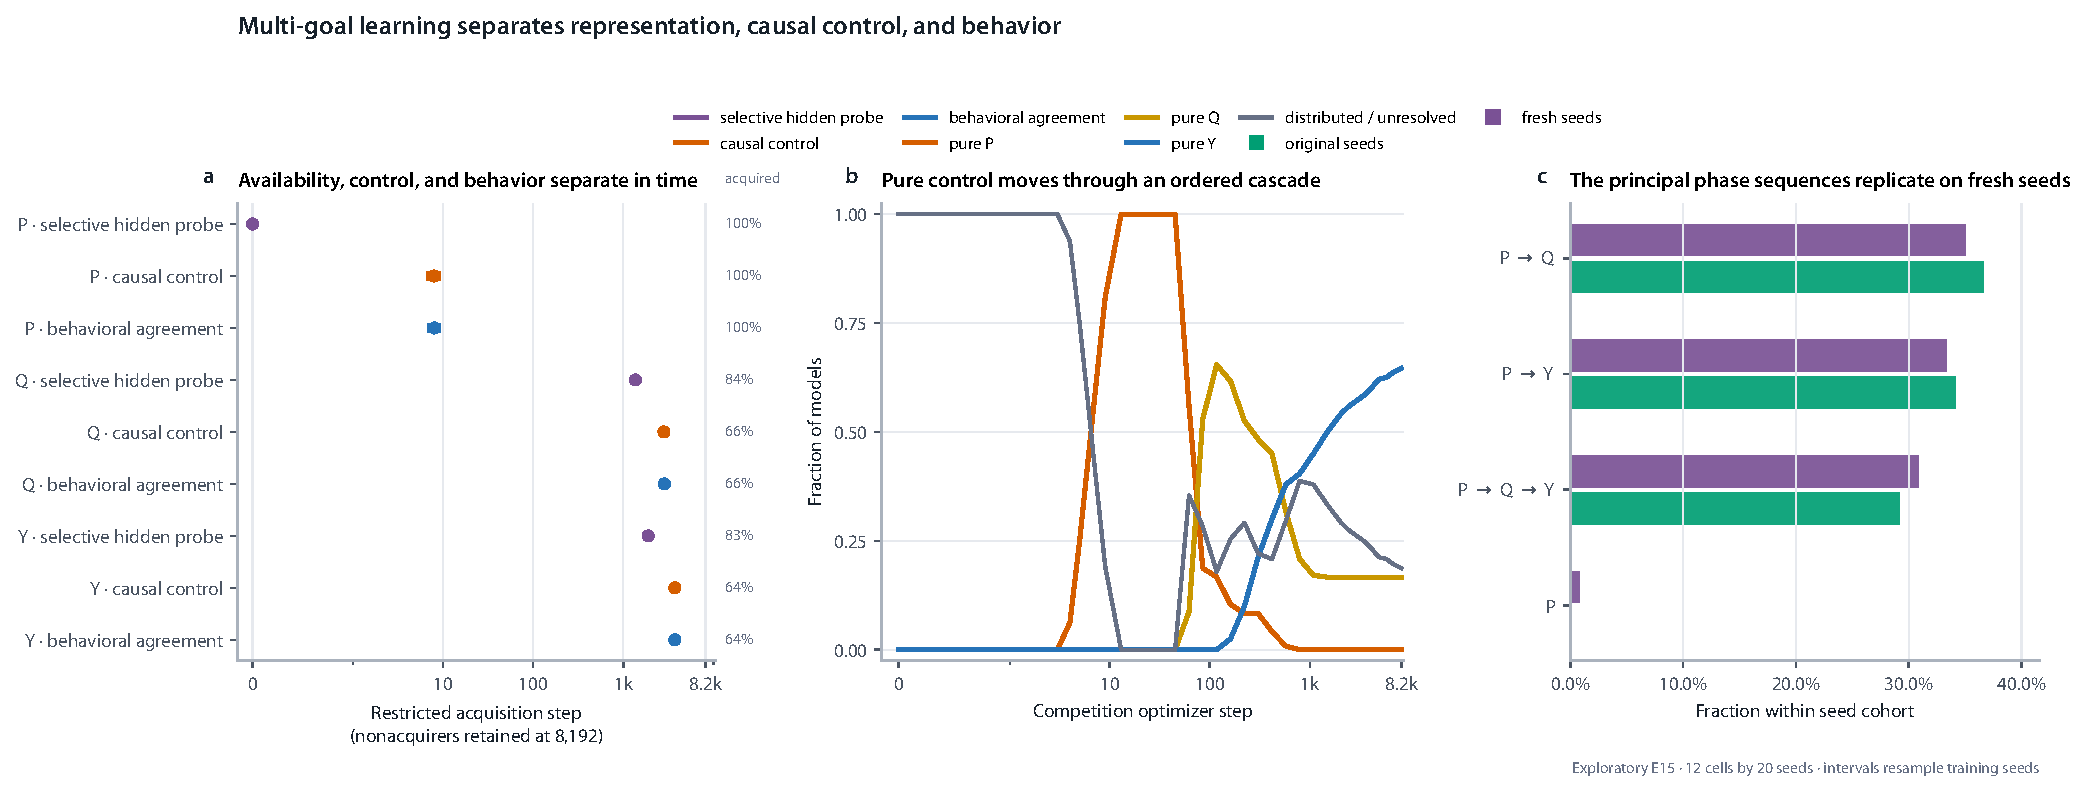
\includegraphics[width=\linewidth,trim=0 18bp 0 25bp,clip]{fig15_multigoal_dynamics.pdf}
  \caption{\textbf{Selective decodability generally precedes control in the adaptive three-goal grid.} \textbf{a}, Horizon-restricted mean acquisition step; non-acquirers remain at 8,192, and the right margin gives the acquired fraction. The selective affine-ridge probe is a decodability measure, not a motivation measure. \textbf{b}, Fraction of models in each persistent pure-control state over training; distributed or unresolved models satisfy no pure label. \textbf{c}, Compressed pure-control sequences in the original and fresh seed cohorts. The grid and analysis are adaptive and post-hoc; intervals, where shown, resample training seeds.}
  \label{fig:multigoal-dynamics}
\end{figure}

\begin{takeaway}
With several plausible goals, learning dynamics can contain an ordered sequence of controlling rules rather than one binary proxy-to-target switch. Selective decodability often precedes behavioral use, but only interventions and disagreement behavior identify when a candidate actually gains control.
\end{takeaway}

\section*{Finding 18: A few disambiguating rows can break a support-perfect gate, but support geometry still matters}

The recurring conditional policy from the previous findings is not irrational on its training distribution. Recall its rule:
\[
g(P,Q,Y)=
\begin{cases}
Y, & P=Q,\\
Q, & P\ne Q.
\end{cases}
\]
When $Q$'s errors are nested inside $P$'s and $q_Q>q_P$, a disagreement means that $Q$ is correct. When the proxies agree, they are either both correct or both wrong, and consulting $Y$ resolves the latter. The gate is therefore perfect on training support. It fails only when $P=Y$ and $Q=-Y$---the missing ``$Q$-only error'' case. Training loss cannot distinguish this gate from the globally correct $Y$ rule until that hole receives some probability mass.

\subsection*{Completing support while holding both proxy accuracies fixed}

We intervene on that support hole in the focal cell where the gate was most common: $q_P=.9$, $q_Q=.95$, degree-two $Q$, degree-five $Y$, width 64, and 10,000 training rows. There are always 1,000 $P$ errors and 500 $Q$ errors. If $m$ denotes the number of $Q$-only-error rows, the four error cells are
\[
\begin{array}{c|cccc}
&\text{both wrong}&P\text{ only wrong}&Q\text{ only wrong}&\text{neither wrong}\\
\hline
\text{count}&500-m&500+m&m&9{,}000-m.
\end{array}
\]
Thus both marginal proxy accuracies remain exact. Moving from zero to $m$ changes exactly $2m$ entries of $Q$: $m$ shared errors are corrected and $m$ previously correct entries become $Q$-only errors. The intended labels, $P$, row order and identities, intended-code channels, nuisance state, padding, initialization, minibatch schedule, and optimizer randomness remain paired within seed. The final active parity bit for $Q$ changes wherever the decoded $Q$ value changes.

The study is adaptive and post-hoc because the focal cell and intervention were chosen after inspecting the temporal panel. Its primary grid was nevertheless fixed before these outcomes were viewed: $m\in\{0,2,10,50,100,250,450\}$ across the same 20 seeds, or 140 runs. A frozen trigger detected the largest registered prevalence drop between $m=2$ and $m=10$ and launched the pre-specified quarter points $m\in\{4,6,8\}$, adding 60 separately identified refinement runs. The zero arm exactly reproduces all shared metrics from the corresponding archived nested-error runs. The fixed exhaustive panels, causal flips, and hidden-state probes are retained, but the endpoint below is defined by behavior across raw codewords; probe accuracy remains evidence of decodability rather than a selected goal.

\subsection*{The gate's 50\% crossing lies between two and five rows}

A stable gate requires modal Boolean signature 113 and at least .90 consistency across the exhaustive candidate truth table. All 20 zero-support runs meet this criterion. The prevalence falls to 13 of 20 at $m=2$, nine at $m=4$, and two at each of $m=6,8,$ and 10; no gate remains at $m\geq50$. A decreasing isotonic fit to the frozen refinement bracket places the linearly interpolated 50\% crossing at $m=3.5$, with a seed-cluster bootstrap interval $[2.0,4.67]$ (\fig{fig:support-completion}a,b). This is a descriptive crossing of prevalence across seeds, not a claim of a mathematically sharp threshold in any individual network.

Target behavior on the held-out $Q$-only panel changes in parallel. Mean target probability rises from .143 $([.099,.190])$ at $m=0$ to .361 $([.270,.448])$ at two rows, .630 $([.537,.720])$ at six, and .979 $([.958,.994])$ at 50. Accuracy on the common, fixed nested-IID panel remains at least .9998 through $m=100$. The intervention therefore changes behavior primarily where the previously supported rule and the intended rule disagree, rather than buying the effect with an ordinary IID collapse.

The unit ``row'' needs care. The two-row arm makes both $Q$-only candidate tuples present, yet 13 of 20 policies still end at the gate; the graded refinement therefore concerns support \emph{mass}, not only presence versus absence. Moreover, each run processes 2,048,000 sampled training examples. The two special rows are presented 409 or 410 times, not twice. The interpolated $m=3.5$ is not a realizable half-row dataset and would correspond to roughly 717 expected presentations under this training schedule. Training seed, not row or presentation, remains the independent unit.

\subsection*{Early learning combines codeword patches with transfer to unseen cases}

The two missing candidate tuples contain 64 possible active $(P,Q,Y)$ codewords. At $m=2$, training covers only two of them. Final target probability is .721 on those seen codewords but .349 on the other 62, compared with .143 on the same unseen set at $m=0$. The much larger seen response shows local fitting, while the improvement on unseen codewords shows transfer beyond memorizing the two exact active patterns. At $m=50$, 54\% of active codewords have appeared; target probability reaches .992 on seen and .966 on unseen codes, leaving a .026 gap $([.008,.053])$. The response is therefore hybrid: highly localized at the smallest doses, then increasingly consistent with the candidate-level intended rule as support expands. Generalization across these synthetic codewords is not evidence of a human-like semantic representation or motivation.

The trajectory also preserves the earlier acquisition cascade (\fig{fig:support-completion}c). At update 33, every dose is essentially pure $P$ and mean $Q$-only target probability is .90. By update 117, $Q$ agreement is approximately one through the moderate doses and the same diagnostic probability has collapsed to about .16. At low and intermediate doses, the explicit conditional gate emerges later: at $m=6$, for example, 17 of 20 runs meet the stable-gate criterion at update 1,085, but only two retain it at 8,192. Larger doses mostly bypass a persistent endpoint and continue toward $Y$. The disambiguating rows therefore do not prevent the early proxies from being learned; they alter whether the later gate persists or the intended rule eventually takes control.

Plotting performance against cumulative presentations of $Q$-only rows does not collapse the dose trajectories (\fig{fig:support-completion}d). A row encountered under a tiny support mass arrives against a different background distribution and at a different stage of optimization than the same cumulative number of presentations under a larger mass. Repetition count alone is consequently not an adequate description of the intervention.

\subsection*{Aggregate dose order hides seed-level reversals and a worse maximal arm}

Stable-gate prevalence decreases monotonically in the aggregate refinement, and mean $Q$-only behavior mostly improves. Individual runs are less orderly. Every seed has at least one adjacent downward fluctuation in target probability across the ten tested doses; 11 have a drop larger than .05, and two lose and later regain the stable-gate label. These are descriptive multiple-dose diagnostics, but they rule out interpreting the aggregate curve as a deterministic per-model transition.

Moderate support is also cleaner than maximal support in this fixed-marginal family. At $m=50$ and 100, all 20 endpoints are pure $Y$. At $m=450$, only 14 are pure $Y$; five are raw-codeword patches and one is another semantic rule, while common-IID accuracy falls to .9876. Increasing $m$ necessarily transfers mass out of both-wrong and neither-wrong cells into the two single-error cells, so the largest arm is not simply ``more copies'' of the moderate intervention. Its four cell counts match the earlier independent-error cell, but its ranked row allocation does not. The count-matched comparison finds no stable-gate difference and only an uncertain +.019 target-probability difference $([-.003,.048])$, so it should not be treated as an exact replay of independent errors.

\begin{figure}[!htbp]
  \centering
  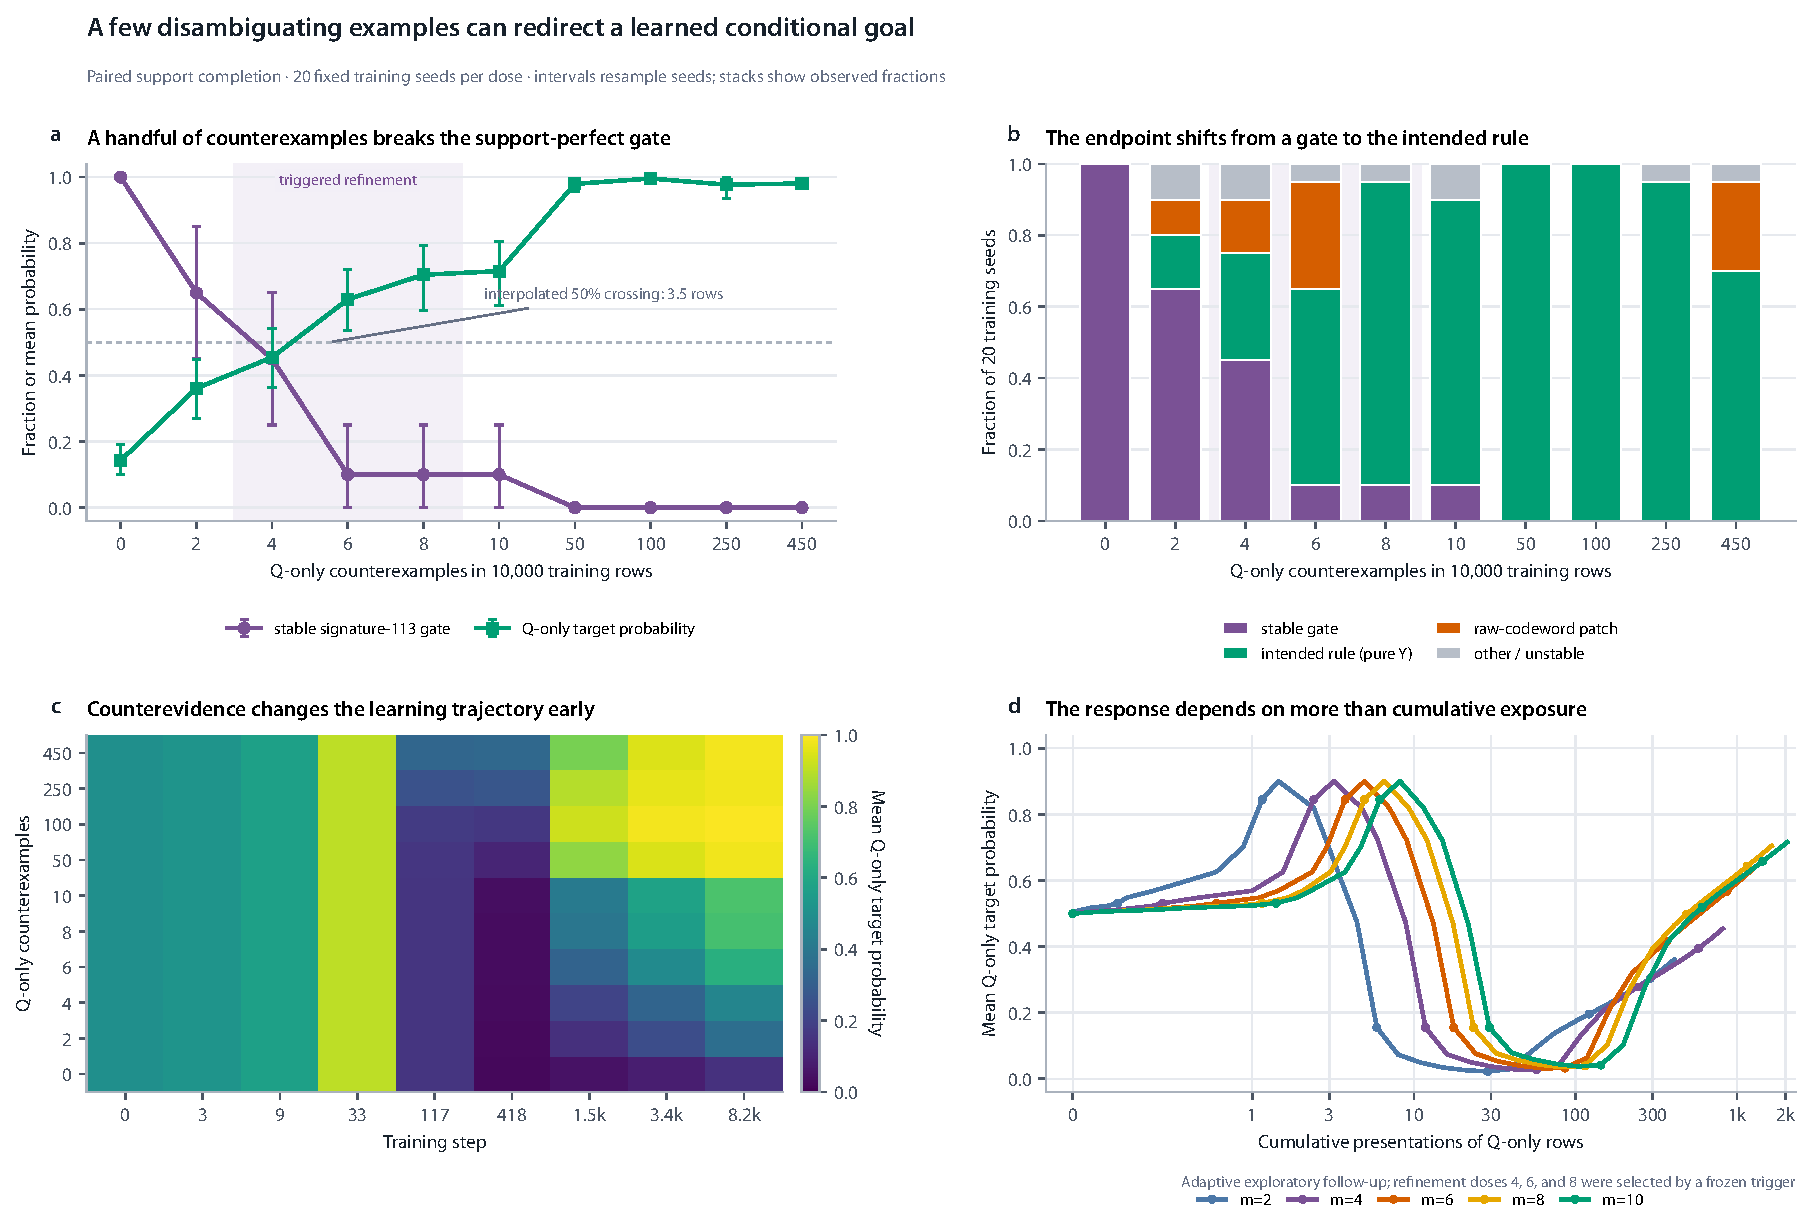
\includegraphics[width=\linewidth]{fig16_support_completion.pdf}
  \caption{\textbf{A small amount of missing-tuple support destabilizes the conditional gate.} \textbf{a}, Stable-gate prevalence and mean target probability on the fixed $Q$-only diagnostic panel. The shaded counts are the triggered refinement; the annotated 50\% crossing is an interpolated across-seed summary. \textbf{b}, Endpoint taxonomy across the 20 paired seeds. \textbf{c}, Mean diagnostic target probability over training: all arms first move toward $P$, then $Q$ or the conditional gate, before support-dependent escape toward $Y$. \textbf{d}, The small-dose trajectories do not align when indexed by cumulative presentations alone. Intervals resample training seeds. The full intervention is adaptive and post-hoc; ``goal'' denotes causal control of this constructed action, not a subjective objective.}
  \label{fig:support-completion}
\end{figure}

\begin{takeaway}
A conditional rule that is perfect on observed support can be causally sustained by a small support hole. Filling that hole redirects many models, but the relevant quantity is repeated support mass and its geometry, not a literal count of one-shot examples or a universal per-model threshold.
\end{takeaway}

\section*{Finding 19: Latent-goal decodability predicts faster handoff after winner knockout, but every model ultimately converges to the exact rule}

A probe-readable candidate is not necessarily controlling the model, but it may still be easier to recruit when the current winner stops working. This distinction matters for predicting behavior after distribution shift. Two models can take the same action for the same causal reason before the shift while differing in which alternative computations their training histories have made accessible. If the winner then becomes uninformative, one model may hand control to an already prepared alternative while another must learn that rule almost from scratch. Conversely, if both adapt equally quickly, earlier probe decodability may have been an epiphenomenal correlate rather than a usable reserve.

\subsection*{Removing the winner's information while keeping it in support}

We test this idea in the same three-candidate selector. Phase A contains a direct proxy $P$ and degree-two encoded proxy $Q$, each 90\% accurate, plus an exact degree-three intended rule $Y$. Width-64, depth-two models receive 45 updates. The only historical contrast changes the overlap of the two proxy-error sets: independent errors make $Q$ more selectively decodable at the branch point, while maximally nested errors make it less so. Twenty new seeds are used throughout. A history enters the paired primary analysis only if $P$ has both behavioral agreement and directional causal control at least .9, with a .1 margin over $Q$ and $Y$, at updates 33 and 45 under \emph{both} error histories. All 20 seeds pass.

Phase B knocks out $P$'s predictive information without moving it off its ordinary input support. Its 10,000 rows form 5,000 pairs. Within each pair the target, $Q$, every active $Q$ and $Y$ code bit, nuisance state, padding, and presence indicators are identical, while $P$ takes opposite signs. Thus $P$ is exactly balanced conditional on every other model input and agrees .5 with both $Q$ and $Y$; $Q$ remains exactly .9 accurate and $Y$ remains exact. Every arm for a seed receives the same phase-B rows, order, and minibatch-index stream for 1,024 updates.

Six trajectories separate history from optimizer state and generic compute: independent-history weights with carried or reset AdamW, nested-history weights with carried or reset AdamW, a scratch initialization, and a 45-update compute sham followed by an optimizer reset. The sham uses paired identical inputs with opposite labels, so its empirical label is unlearnable conditional on the complete input. Deterministic CPU replays require exact initial, final-model, final-optimizer, data, sampler, and phase-A measurement hashes before a historical branch is accepted.

At every phase-B checkpoint, an exhaustive factorial panel measures candidate behavior, directional causal control, hidden-state probes, and the full Boolean truth table. A $Q$ handoff requires two consecutive checkpoints at which both $Q$ behavior and $Q$ causal score are at least .9 and exceed the corresponding $P$ and $Y$ measurements by .1. The primary outcome avoids threshold timing: it is the update-weighted area from zero through the directly observed update 128 under the mean of $Q$ behavior and $Q$ causal control, normalized to $[0,1]$.

\subsection*{A more decodable alternative takes control sooner}

The intended representation-history manipulation is present at the branch point. Independent rather than nested errors raise selective final-hidden $Q$ probe accuracy by .1664 $([.1512,.1816])$. The paired differences in $P$ behavior, $P$ causal control, and raw $Y$ probe accuracy are $-.0045$, $-.0046$, and $-.0090$; all three intervals lie inside the fixed $\pm.05$ specificity band. The two histories therefore begin phase B with nearly identical $P$ control and a large difference in $Q$ accessibility, although the small co-shifts are real and the manipulation changes the broader training distribution rather than a probe coordinate alone.

With AdamW reset in both arms, independent history raises $Q$-control area through update 128 by .0596 $([.0495,.0721])$ relative to nested history (\fig{fig:winner-knockout}a--b). It also shortens the restricted mean confirmation time by 73.35 updates: the signed paired contrast is $-73.35$ $([-171.55,-22.85])$. Independent-history models confirm $Q$ handoff after 27.7 updates on average, compared with 101.05 for nested-history models. Nineteen of 20 nested-reset models confirm the event; seed 229 proceeds directly to $Y$ and remains right-censored for $Q$ at 1,024. This one run enlarges the timing contrast, which is why the fully observed area result is the more stable primary evidence.

The same independent-history reset is also faster than learning from scratch or after generic sham compute. Its area advantages are .0550 $([.0407,.0696])$ and .0660 $([.0483,.0843])$; its restricted-time contrasts are $-16.35$ $([-18.8,-14.1])$ and $-16.95$ $([-20.35,-14.0])$. Scratch and sham controls confirm $Q$ at mean updates 44.05 and 44.65. These comparisons show a reusable effect of learned weights or representations, but they are not clean $Q$-specific history contrasts: unlike the historical arms, scratch and sham models do not begin phase B under strong $P$ control.

Carrying optimizer moments contributes little on the registered scale. Carry-minus-reset $Q$-area effects are $-.0018$ $([-.0073,.0029])$ after independent history and $-.0100$ $([-.0172,-.0036])$ after nested history. The latter is detectably negative but far below the pre-specified .05 materiality threshold; both area intervals lie inside $\pm.05$, and both restricted-time intervals lie inside $\pm16$ updates. The speed advantage is therefore associated primarily with learned weights and representations rather than AdamW state.

\subsection*{The prepared proxy is a waypoint, not the endpoint}

The intervention reveals a three-stage succession rather than permanent transfer to $Q$. Every historical model begins phase B in $P$ control and confirms that state at update one. All 40 independent-history trajectories and 38 of 40 nested-history trajectories then confirm $Q$ before $Y$; the remaining nested seed appears in both carry and reset branches and goes from $P$ directly to $Y$. Scratch and sham models instead follow $Q\mathbin{\to}Y$. By update 1,024, every one of the 120 models has exact-$Y$ Boolean signature 85, pure behavioral-and-causal $Y$ control, and perfect factorial target accuracy. The inherited $Q$ representation predicts how quickly a model traverses the middle regime, not its eventual destination.

More preparation for $Q$ also makes that middle regime last longer. At phase-B update zero, mean raw final-hidden $Q$ probe accuracy is .960 after independent history, .783 after nested history, .668 from scratch, and .638 after sham compute. Yet mean persistent-$Y$ confirmation occurs at updates 311.4, 246.45, 205.55, and 199.2 in the same reset-arm order. Relative to independent history, nested, scratch, and sham histories therefore reach $Y$ 64.95 $([44.75,84.26])$, 105.85 $([78.55,134.25])$, and 112.20 $([79.25,143.45])$ updates sooner. These $Y$ timings are exploratory secondary outcomes and inherit the checkpoint threshold's discretization, but their ordering is consistent with a prepared intermediate proxy delaying intended-rule takeover rather than accelerating alignment. Continued exact evidence eventually overcomes it in every observed run.

This result supplies a functional test that the earlier probe ordering lacked: accessibility measured before the shift predicts later causal control under winner knockout. It still does not establish that linear probe decodability itself is the causal mediator. Independent and nested error histories change support geometry and all gradients accumulated during phase A; the probe difference is a measured consequence of that intervention. Directly editing the $Q$ representation while holding the rest of history fixed would be needed to isolate probe-readable information from other prepared circuitry.

\begin{figure}[!htbp]
  \centering
  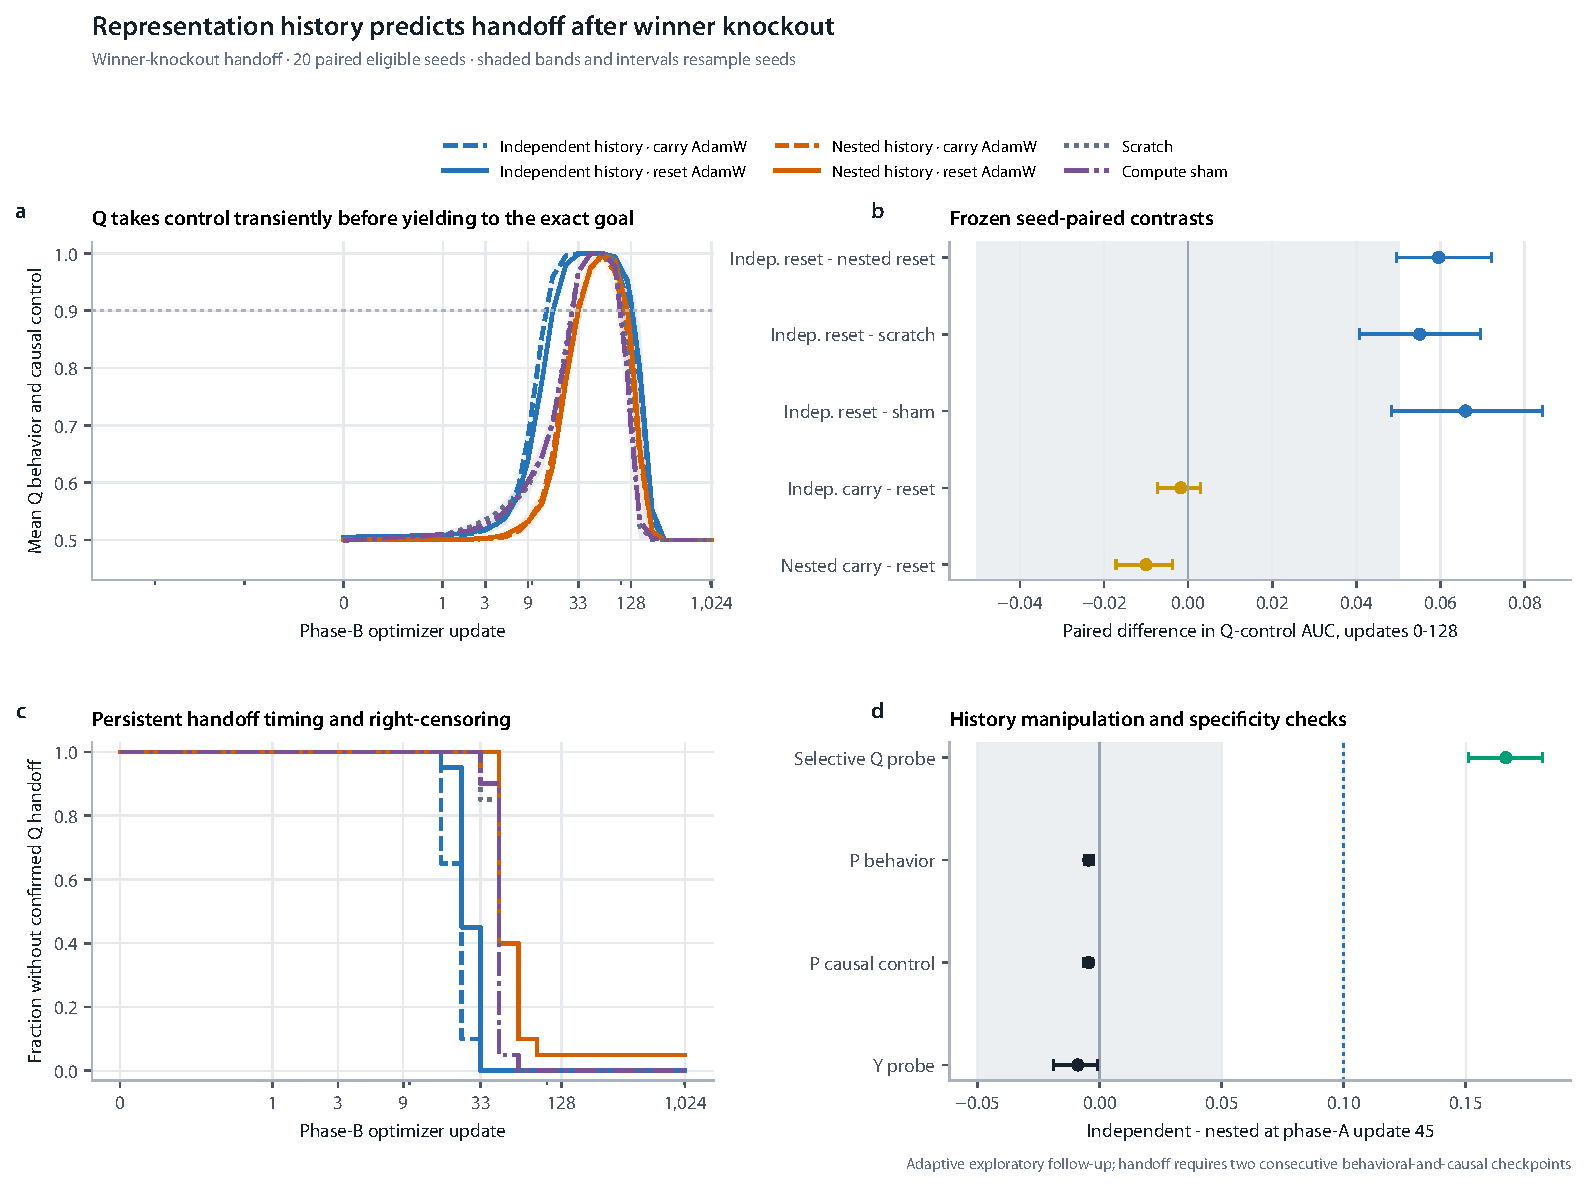
\includegraphics[width=\linewidth]{fig17_winner_knockout.pdf}
  \caption{\textbf{Representation history predicts functional handoff after winner knockout.} \textbf{a}, Mean $Q$ behavior and causal control rises sooner after independent-error history, then falls as every arm transfers to exact $Y$. \textbf{b}, Frozen paired contrasts in $Q$-control area through update 128; the gray band marks $\pm.05$ practical equivalence. \textbf{c}, Fraction of paired-eligible seeds without a confirmed two-checkpoint $Q$ handoff; one nested-history seed is right-censored. \textbf{d}, The phase-A manipulation produces a large selective-$Q$ probe difference while the $P$ behavior, $P$ causal, and raw-$Y$ probe intervals remain inside the specificity band. Bands and intervals resample training seeds. The experiment is adaptive and post-hoc.}
  \label{fig:winner-knockout}
\end{figure}

\begin{takeaway}
Probe-decodable information can be functionally prepared rather than merely visible to an observer: after the current winner loses predictive value, the history with more accessible $Q$ hands control to $Q$ sooner and sustains that intermediate proxy longer. Continued exact evidence ultimately moves every model to $Y$, but preparation for a backup proxy delays rather than accelerates that intended takeover.
\end{takeaway}

\section*{Finding 20: Deeper mazes change local goal control before errors compound across forks}

Repeating a decision along a route can reduce success for two distinct reasons. Even if the same goal controls every local choice with accuracy $a$, reaching the correct leaf after $D$ irreversible forks should occur only about $a^D$ of the time. But a deeper route can also make each local decision harder: the selector must identify the current stage, retrieve the corresponding semantic channels, and learn each stage from a smaller share of a fixed update budget. The first effect compounds an unchanged policy; the second changes which rule the policy uses.

RouteWorld separates these mechanisms. It embeds a perfect binary tree in a wall grid with equal-length corridors and indistinguishable terminal leaves. Depths one, two, and four contain $2,4,$ and $16$ leaves. The depth-four maze is $13\times33$, and every root-to-leaf rollout takes 27 primitive moves. A scripted controller executes forced corridor moves and asks the shared learned selector for a left--right bit only at the $D$ true junctions. Thus collision or pathfinding error cannot masquerade as goal error.

The selector sees the proxy and parity channels for the full route plus a one-hot stage address. It does not see a marked target, node identity, or its previous choices. This is a stage-indexed shared decision rule rather than a learned history-conditioned planner. We cross depth $D\in\{1,2,4\}$, proxy accuracy $q\in\{.75,.95,.99\}$, parity degree $k\in\{2,4\}$, widths 16 and 64, and ten seeds. One arm fixes training at 1,024 updates. The other uses $1{,}024D$ updates so that each stage receives approximately the depth-one number of sampled rows. The two depth-one arms are deterministic duplicates and are retained as paired controls, not independent replications.

\subsection*{More updates per fork recover part, but not all, of the local goal shift}

At one fork, mean all-conflict branch accuracy is .892 and exact-rule flip sensitivity is also .892. With a fixed total budget, branch accuracy falls to .656 at two forks and .346 at four. Scaling total updates with depth improves those values to .722 and .518 (\fig{fig:routeworld}a). At depth four, the paired improvement is .172 $([.155,.188])$, recovering about 31\% of the fixed-budget depth loss. The causal exact-rule flip rate rises by a nearly identical .173 $([.157,.189])$, while proxy influence falls, showing that the longer training regime changes rule control rather than merely confidence. This arm both restores the expected number of sampled rows per stage and lengthens the total optimization horizon, so it does not isolate data exposure from additional sequential optimization.

The longer regime does not restore the depth-one policy. Even after updates scale per fork, depth four is .374 $([.352,.394])$ lower in branch accuracy than depth one, and exact-rule flip sensitivity is .396 $([.375,.417])$ lower. The endpoint cells make the boundary concrete: with $q=.75,k=2$, depth-four selectors remain perfectly intended-controlled; with $q=.99,k=4$, their mean intended branch accuracy is .004 and proxy flips change .993 of decisions. Route depth therefore interacts with the same proxy-fidelity and rule-accessibility boundary found in the one-step task.

The residual depth cost is not evidence of difficult physical navigation. The model interface is padded to a fixed maximum width, but a deeper route activates more stage-specific channel blocks and requires the stage address to route among them. In the longer regime, reversing the address produces mean within-run absolute branch-accuracy shifts of .422 at depth two and .393 at depth four; removing it produces shifts of .212 and .271. The corresponding signed shifts are $-.177,+.025,-.090,$ and $+.024$, because disrupting the mapping pushes intended-controlled and proxy-controlled cells toward chance in opposite directions. Stage-local channel interventions have much larger effects at the addressed fork than elsewhere, yet flipping one stage's feature still changes about 6\% of other-stage decisions on average. This imperfect isolation is consistent with a learned multiplexing problem becoming part of goal selection.

Single-conflict panels make the localization visible. At depth four in the longer regime, accuracy at the one challenged stage is only .564, while accuracy at the three nonconflicted stages remains .994. Under the fixed budget those values are .375 and .996. The nonconflicted stages are easy precisely because $P=Y$ there, so their accuracy does not identify which rule controls them. Averaging all four stages would give the much less informative .887 and .840, respectively, because those three nondiagnostic stages dilute the decision on which the candidate goals actually disagree. The challenged-stage result is therefore the relevant diagnostic: the policy executes most ordinary choices correctly while changing which rule controls the fork where the candidates separate.

\subsection*{Whole-route success is then predicted by ordinary compounding}

The longer-regime mean whole-route success falls from .892 at depth one to .674 at depth two and .384 at depth four, below its corresponding branch accuracies. The registered compounding approximation raises each run's pooled branch accuracy to the power $D$. Across the complete grid, observed success exceeds that prediction by .0011 $([-.0011,.0033])$, providing no detectable signed departure. Because the stages need not be equally difficult, we also examined an explicitly exploratory refinement that multiplies their separate accuracies. Restricting that estimate to depths greater than one, where compounding is nontrivial and the depth-one duplicate control cannot shrink the average, observed success exceeds the refined prediction by .0080 $([.0042,.0117])$; the mean absolute run-level gap is .0176 $([.0144,.0206])$. Figure~\ref{fig:routeworld}b shows the stage-product and observed curves nearly superimposed. Forty-four of the 48 depth-greater-than-one design cells have an absolute mean gap no larger than .05. Three exceptions are depth-two $q=.99,k=2$ cells with positive dependence; the fourth is a depth-four $q=.95,k=2$, width-64 cell with negative dependence. Compounding is therefore a strong aggregate approximation rather than an exact independence law.

All scripted physical rollouts reach a leaf without collision, and every rollout's success exactly matches the route implied by the selector's vector of branch decisions. These rollouts validate the maze and accounting. They are repeated evaluations of the same trained seed, not new samples of learned planning ability.

\begin{figure}[!htbp]
  \centering
  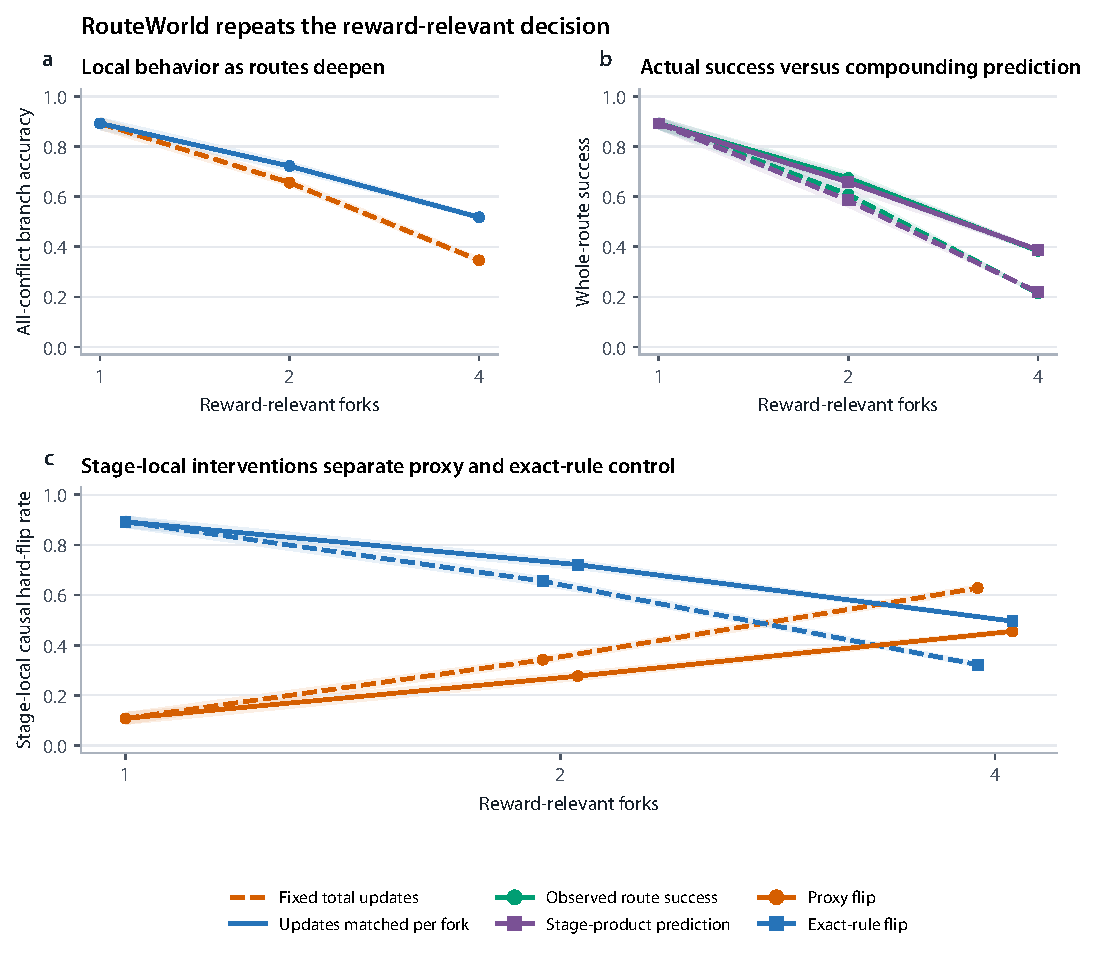
\includegraphics[width=\linewidth]{fig13_routeworld_followup.pdf}
  \caption{\textbf{Route depth changes local goal control and then compounds the remaining errors.} \textbf{a}, All-conflict branch accuracy declines with depth; matching updates per fork recovers only part of the loss. \textbf{b}, Whole-route success closely follows the exploratory product of stage-specific branch accuracies; the registered pooled branch-accuracy power is reported in the text. \textbf{c}, Stage-local causal flips show exact-rule control giving way to proxy control as routes deepen. Lines collapse $q$, degree, width, and seeds; bands are 95\% seed-bootstrap intervals.}
  \label{fig:routeworld}
\end{figure}

\begin{takeaway}
Adding independently encoded, stage-indexed decisions can alter local goal control even when expected per-stage presentations are matched. Given those local predictions, end-to-end success in the scripted maze is largely captured by compounding.
\end{takeaway}

\section*{Finding 21: A narrow first-layer input pathway causally changes how quickly a proxy takes over}

The winner-knockout experiment showed that an independently distributed error history leaves the encoded proxy $Q$ more selectively decodable and lets it take control sooner than a nested-error history. That comparison was informative but broad: changing error overlap changes every gradient in the first phase and can consequently alter every layer of the network. The association between decodability and takeover could therefore reflect a usable $Q$ representation, some other difference between the two trained networks, or both.

A useful causal test should change a small piece of the prepared $Q$ computation without changing the rest of the model. The first affine layer provides such a target. Its two active $Q$ columns are the only direct routes by which the encoded proxy bits enter the network. If learning in those columns contributes to later adaptability, returning them to their initial values should make $Q$ slower to recruit after $P$ is knocked out. Conversely, moving the independently trained columns into a nested-history model should make $Q$ easier to recruit. Neither intervention is expected to delete or install an entire goal: biases and downstream weights remain untouched, and phase-B training can relearn the edited pathway.

\subsection*{Restoring and transplanting the active input columns}

We returned to the same fixed cell: a direct proxy $P$ and degree-two encoded proxy $Q$ are each 90\% accurate, degree-three $Y$ is exact, and width-64, depth-two models train for 45 phase-A updates. Twenty further fresh seeds each generate an independent-error history and a maximally nested-error history from the same initialization. Every history is purely $P$-controlled at the two frozen pre-edit checkpoints.

For the independent model, we restore the $64\times2$ block carrying $Q_1,Q_2$ to its initialization. For the nested model, we transplant the corresponding block from the paired independent model. Each edit changes exactly 128 first-layer weights. A matched sham applies the exact same signed 128-value displacement to two model-visible random-padding columns that are inactive for the candidate goals, while a no-op branch retains the recipient weights. Thus the six branches are independent no-op, active restore, and padding sham, together with nested no-op, active transplant, and padding sham. The shams control displacement values, norm, parameter count, and layer; they do not assume that perturbing goal-inactive random padding has the same feature geometry as perturbing $Q$.

After surgery, every branch receives a fresh empty AdamW optimizer and the same paired phase-B rows, minibatch order, and sampler stream. Phase B makes $P$ exactly uninformative conditional on every other input, retains $Q$ at 90\% accuracy, and keeps $Y$ exact. The primary outcome is the update-weighted area through directly observed update 128 under the mean of $Q$ behavioral agreement and directional causal control. This continuous outcome measures early recruitment without making the conclusion depend on a checkpoint crossing.

This study is adaptive and post-hoc. We first inspected five archived winner-knockout seeds, which fixed the layer, coordinates, six branches, area outcome, thresholds, and controls; those seeds are excluded from every estimate here. The design was then frozen before a three-seed manipulation-only pilot and the 20 further fresh seeds. Each active-edit direction required a mean paired area effect of at least .02, a paired seed-bootstrap interval above zero, and at least 15 positive seed differences. Each padding-sham-minus-no-op interval also had to lie wholly inside $[-.01,.01]$. The full-panel manipulation check separately required selective-$Q$ probe-advantage shifts of at most $-.05$ for restoration and at least $+.05$ for transplantation, with all sham-$Q$ and frozen $P/Y$ intervals inside $[-.05,.05]$. ``Frozen'' describes the internal sequence of this selected follow-up; these intervals are neither preregistered nor family-wise confirmatory.

\subsection*{The active edits move both decodability and subsequent control}

All 20 paired seeds remained eligible, and all 120 post-edit branches remained purely $P$-controlled. Restoring the active columns reduced selective final-hidden $Q$ probe advantage---held-out accuracy minus its matched permuted-label control---by .1058, 95\% \CI{} $[-.1205,-.0916]$, relative to the paired independent no-op. Transplanting them increased it by .0751, $[.0694,.0813]$, relative to the paired nested no-op. The corresponding padding-sham shifts were $-.0343$ $([-.0421,-.0274])$ and $-.0105$ $([-.0147,-.0065])$ (\fig{fig:q-input-pathway}a). These sham effects are not literally zero, but both satisfy the frozen $\pm.05$ equivalence criterion. For every edit, the intervals for $P$ behavioral agreement, $P$ directional causal control, selective $P$ probe advantage, and selective $Y$ probe advantage also lie within that band.

The later control results move in the same two directions (\fig{fig:q-input-pathway}b--d; \tbl{tab:q-input-pathway}). In independent-history models, the padding sham has mean $Q$-control area .9372, compared with .9010 after active restoration, giving a frozen restoration contrast of +.0361 $([.0296,.0432])$. In nested-history models, transplantation raises area from .8824 under the padding sham to .9116, giving a frozen transplantation contrast of +.0293 $([.0249,.0339])$. All 20 paired differences are positive in both directions, so both active contrasts clear the fixed .02 effect threshold, interval rule, and 15-of-20 sign rule.

\begin{figure}[!htbp]
  \centering
  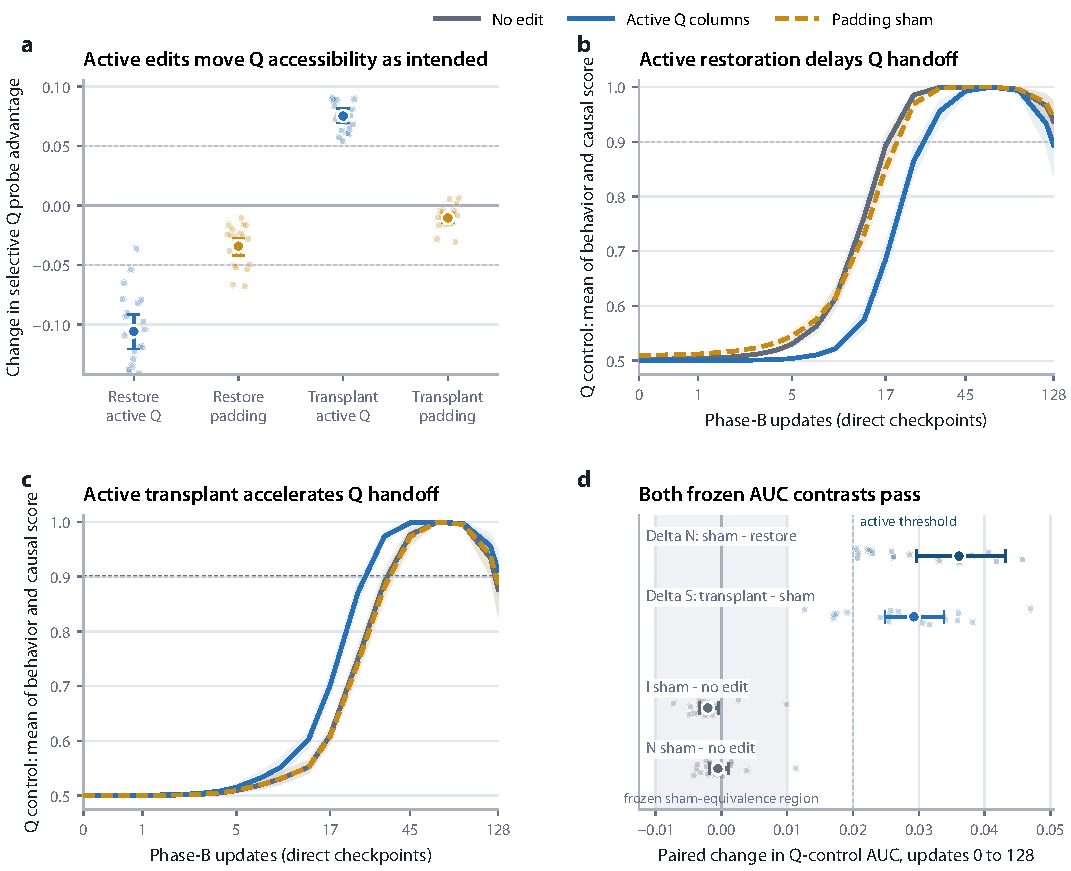
\includegraphics[width=\linewidth]{fig19_active_q_pathway.pdf}
  \caption{\textbf{Active first-layer $Q$ inputs contribute to later proxy takeover after winner knockout.} \textbf{a}, Post-edit change in selective final-hidden $Q$ probe advantage relative to the paired no-op; the score is held-out accuracy minus its matched permuted-label control. Pale points are the 20 fixed full-panel seeds; large points and bars show means and paired seed-bootstrap 95\% intervals. Dotted horizontal lines mark the frozen $\pm.05$ manipulation and sham-equivalence bounds. \textbf{b}, Mean $Q$ control after restoring the independent-history active columns to initialization. \textbf{c}, The corresponding trajectory after transplanting the independently prepared columns into the nested-history model. $Q$ control is the mean of behavioral agreement and directional causal score; bands resample seeds, and every plotted value is a direct checkpoint. \textbf{d}, The two frozen active AUC contrasts and both sham-minus-no-op checks through update 128. The blue dotted line marks the +.02 active-effect threshold and the gray region marks the $[-.01,.01]$ sham-equivalence interval. The intervention identifies a contribution of these active input columns, not mediation by a probe statistic or a complete $Q$ circuit.}
  \label{fig:q-input-pathway}
\end{figure}

\begin{table}[!htbp]
\centering
\small
\begin{adjustbox}{max width=\linewidth}
\begin{tabular}{llrr}
\toprule
Recipient history & Branch & Mean $Q$ area, 0--128 & Paired frozen effect \\
\midrule
Independent & no-op & .9392 & --- \\
Independent & padding sham & .9372 & --- \\
Independent & active-$Q$ restore & .9010 & $+.0361\;[.0296,.0432]$ \\
\addlinespace
Nested & no-op & .8829 & --- \\
Nested & padding sham & .8824 & --- \\
Nested & active-$Q$ transplant & .9116 & $+.0293\;[.0249,.0339]$ \\
\bottomrule
\end{tabular}
\end{adjustbox}
\caption{\textbf{Editing the first-layer $Q$ columns changes early $Q$ control after winner knockout.} Area is the normalized linear-in-update AUC through phase-B update 128 of the mean of behavioral and directional-causal $Q$ control. The restoration effect is padding sham minus active restore; the transplantation effect is active transplant minus padding sham. Intervals resample the 20 paired training seeds.}
\label{tab:q-input-pathway}
\end{table}

The shams make the result difficult to explain as damage from changing a first-layer tensor. Independent padding-sham minus no-op area is $-.00205$ $([-.00331,-.00041])$, and nested padding-sham minus no-op area is $-.00051$ $([-.00178,.00112])$. Both intervals lie inside the frozen $\pm.01$ band. The former is detectably negative at this precision, but it is practically equivalent by the rule fixed before the fresh pilot. Auxiliary activation audits also find nearly matched first-layer perturbation scales: relative preactivation RMS is .199 for both independent active and sham edits and .109 for both nested edits; mean ReLU-state flip rates are .059 versus .060 and .030 versus .033, respectively.

Checkpoint-defined timing gives the same secondary picture. Mean confirmation of persistent $Q$ control occurs at update 44.55 after restoration versus 31.65 after its sham, a delay of 12.90 updates. Transplantation confirms at 42.85 versus 57.50 after its sham, an advance of 14.65 updates. Every branch nevertheless reaches the exact $Y$ rule by update 1,024. The earlier mean $Y$ confirmation after weakening $Q$ (277.95 versus 303.10) and later confirmation after strengthening it (299.00 versus 277.95) are descriptively consistent with $Q$ acting as an intermediate competitor rather than the endpoint. These timing comparisons are secondary and inherit the coarse direct-checkpoint lattice.

\subsection*{The intervention identifies a pathway contribution, not a mediator}

The bidirectional result narrows the earlier history association. Learned weights on the two active first-layer $Q$ inputs contribute causally to how quickly $Q$ gains behavioral and directional-causal control after $P$ loses its information. Returning those weights toward their untrained state delays takeover; placing the prepared weights into the less prepared recipient accelerates it; an equal tensor displacement on goal-inactive random-padding coordinates does neither to a material degree.

The result does not show that selective probe advantage mediates the history effect, and it does not identify a unique or complete $Q$ circuit. Restoration leaves all downstream weights intact, transplantation places donor columns into a recipient with a different internal history, and a matched padding sham cannot reproduce the active coordinates' semantic geometry. The natural no-op independent-minus-nested area gap is .0563, while the two edits are recipient-specific nonlinear interventions rather than terms in an additive decomposition. Reporting their ratio as a ``mediated fraction'' would therefore be unjustified. Persistent takeover after restoration shows that the phase-A values in these columns are not permanently required. The columns remain trainable during phase B, so input-path necessity was not tested, and transplantation did not install immediate $Q$ control. The interventions instead change the rate at which subsequent training recruits one usable component of preparation that it can bypass or rebuild.

\begin{takeaway}
Editing the two active first-layer $Q$ input columns changes how quickly subsequent winner-knockout training recruits $Q$ in both directions, while matched random-padding edits leave $Q$-control area practically unchanged. This identifies a contribution from those columns, not a complete $Q$ circuit or a mediated fraction of the history effect.
\end{takeaway}

\section*{Finding 22: Reordering identical cumulative evidence leaves different goals in control}

Sequential learning is often framed as forgetting: later data can overwrite behavior supported by earlier data \citep{kirkpatrick2017forgetting}. That observation leaves a stricter ambiguity. If several rules are individually learnable and two models eventually receive exactly the same labeled examples, their behavior may still depend on the order in which those examples arrived. Ordinary training traces cannot isolate this possibility because later checkpoints usually differ in both chronology and cumulative evidence.

An earlier engineering attempt stopped before its full panel because each intended diagnostic block admitted the same exact inverse-proxy shortcut. The repaired construction was designed after that failure and is therefore adaptive and post-hoc, although its engineering gate, primary outcome, hierarchy, seeds, and analysis were frozen before their respective outcomes. It uses the direct rule $P$, degree-two parity $Q$, and degree-three parity $Y$ on the same exhaustive set of 64 raw codewords. Each goal-specific component labels every codeword by one candidate rule. Its weights make the requested rule exact within that component and either other named rule accurate only at chance. After all three components are pooled, each named rule attains the same $2/3$ accuracy, which is also the upper bound for any function of the complete model input.

\subsection*{The same complete evidence arrives in all six orders}

For each seed, six models begin from a bit-identical initialization and receive all permutations of the three components:
\[
P\!-!Q\!-!Y,\quad P\!-!Y\!-!Q,\quad
Q\!-!P\!-!Y,\quad Q\!-!Y\!-!P,\quad
Y\!-!P\!-!Q,\quad Y\!-!Q\!-!P.
\]
Every component contributes 256 updates, and a fresh empty AdamW optimizer is installed at each boundary while model weights continue. At update 768, every schedule has received exactly the same 221,184 labeled sample presentations; only their order differs. The experimental seed changes the initialization but not the data, component streams, or phase randomness. Twenty fresh seeds each contribute all six paired schedules, giving 120 full-panel trajectories.

All schedules then receive another fresh optimizer and the same 256-update washout. This washout contains only the 16 raw codewords on which $P=Q=Y$, labeled by their common action. It continues training without adding evidence that favors one named rule on a disagreement. Fresh optimizers rule out carried AdamW moments as the source of any schedule effect, while the continuing model weights retain the path by which each solution was reached.

\subsection*{The last block wins, rather than producing a smooth recency gradient}

Before the order comparison was authorized, an outcome-blind nine-artifact pilot required the same seed to acquire stable pure $P$, $Q$, and $Y$ control in three isolated components; all three pilot seeds passed. In the full panel, every one of the 360 goal-specific blocks ended with the exact requested 64-bit action table. Immediately before washout, the last component therefore controls all 120 schedules exactly: 40 implement $P$, 40 implement $Q$, and 40 implement $Y$.

The registered primary measure takes the mean pairwise Hamming distance among the six exhaustive action tables within each seed, then integrates it over directly observed washout offsets 33 through 128. Its normalized mean area is .39835, 95\% \CI{} $[.39588,.39980]$, and all 20 seeds clear the fixed material boundary. For scale, two schedules ending in each of the three pure rules produce dispersion .40. The measured effect is therefore 99.6\% of the pure last-goal pattern.

The signed hierarchy identifies which part of the order matters. Last-presented minus first-presented control has mean area .99449 $([.98620,.99936])$, with a positive, material value in all 20 seeds. Bonferroni-adjusted last-minus-first areas are .99227 for $P$, .99924 for $Q$, and .99195 for $Y$, with all three intervals excluding zero. By contrast, middle-minus-first areas are approximately zero for every goal, while last-minus-middle areas are .992 or larger. The effect is thus winner-take-last rather than a gradual ordering from first through middle to last.

This separation is invisible to pooled accuracy. At every one of the 2,400 schedule--checkpoint observations during washout, accuracy on the pooled three-component evidence is exactly $2/3$, and accuracy on the concordant washout rows is exactly one. The hard policies can differ nearly maximally because every non-unanimous codeword is tied in the pooled labels. Continued agreement-only training sharpens confidence without resolving those ties: mean pooled binary cross-entropy rises from 2.526 at washout entry to 3.527 at its end even though $0$--$1$ accuracy remains fixed.

Common training removes little of the behavioral separation (\fig{fig:identical-order}). Mean truth-table dispersion moves from .4000 at washout entry to .3970 at offset 128 and .3958 at offset 256; the registered signed recency margin moves from 1.000 to .990 and .986. At the final checkpoint, 40 of 40 $P$-last schedules, 39 of 40 $Q$-last schedules, and 32 of 40 $Y$-last schedules still implement the exact named table. The other nine are raw-codeword-specific composites, but eight remain pure by the broader behavioral-and-causal threshold, leaving 119 of 120 policies under their last goal's control.

\begin{figure}[!htbp]
  \centering
  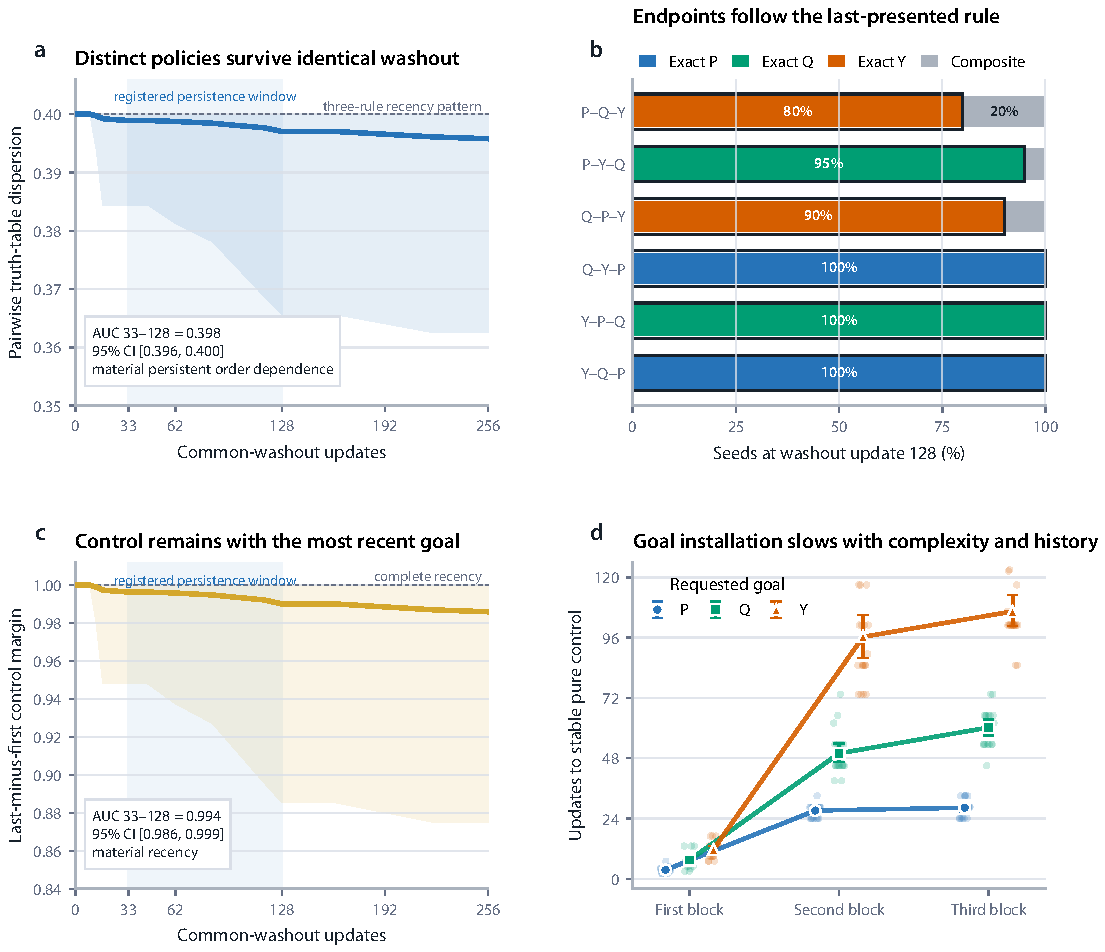
\includegraphics[width=\linewidth]{fig20_identical_evidence_order.pdf}
  \caption{\textbf{Identical cumulative evidence preserves a nearly pure last-goal effect.} \textbf{a}, Mean pairwise Hamming dispersion among the six schedule-specific truth tables during the common washout; the pale band is the full range across 20 seeds and the blue region marks the registered area window. The .40 reference is the exact pattern with two schedules controlled by each last-presented rule. \textbf{b}, Exact truth-table classes at washout offset 128. Each row contains 20 seeds, and the outlined segment is the rule presented last. \textbf{c}, Mean last-minus-first behavioral-and-causal control margin during washout, again with the full seed range. \textbf{d}, First checkpoint in each persistent pure-control pair, averaged within seed over the two schedules placing a requested rule at each position; bars are 95\% seed-bootstrap intervals and pale points are seed means. Acquisition timing is a secondary, checkpoint-discretized description rather than part of the registered order test.}
  \label{fig:identical-order}
\end{figure}

\subsection*{Goal replacement repeats, but a universal probe sequence does not}

The component trajectories do support a weak form of repeated goal acquisition. Every requested rule takes pure behavioral and directional-causal control in all 360 blocks. The median first persistent pure-control offsets are 7, 45, and 62 for blocks one, two, and three. Within those positions, the corresponding descriptive medians for $P$ are 3.5, 24, and 24; for $Q$, 7, 45, and 62; and for $Y$, 13, 85, and 117. Replacing an established controller is therefore slower than learning from initialization, and the penalty grows with the rule's model-relative difficulty.

The transition is usually not a direct jump between named rules. Blocks two and three always begin under the immediately preceding goal and end under the requested one, but 231 of their 240 replacements pass through at least one checkpoint with no pure controller. Most intermediate tables are codeword-specific composites. None of the 9,600 component and washout truth-table observations equals the fixed candidate-majority rule, and no replacement visits the third named rule as an intervening pure controller. The recurring pattern is old rule, distributed or patched behavior, then new rule---with occasional returns to the old or nascent new rule on the coarse checkpoint lattice.

The stronger proposal that probes, behavior, and causal control should always appear in that order does not survive this panel. Across the 360 requested blocks, the first-hidden probe precedes behavior in 225 cases, coincides in 50, and follows it in 85; the final-hidden counts are 177, 90, and 93. Pooling both layers, probe availability is no later than behavior in 97.5\% of the direct-$P$ observations, 75.0\% for $Q$, and only 53.3\% for parity-coded $Y$. The step-zero $P$ event is especially weak evidence of acquisition because the direct input is already linearly recoverable from random hidden features.

Behavioral, directional-causal, and pure-control event status and timing coincide in all 2,160 candidate--layer rows, so this experiment cannot resolve separate behavioral and causal phases at all. The robust generalization is repeated goal replacement, not a universal internal phase sequence. Probe timing remains dependent on the layer, candidate complexity, threshold, and checkpoint spacing.

The pooled objective deliberately leaves disagreement codewords underdetermined, and the washout never adjudicates among the candidates there. These results establish path dependence under this exact construction, not persistence against uniquely identifying negative evidence. Reordering whole components also reorders their component-specific raw-input frequencies together with their labels, so the intervention does not isolate label order alone.

\begin{takeaway}
The multiset of training examples is not enough to predict goal control when the pooled evidence admits several equally accurate rules. Here the most recent complete evidence block determines behavior through a shared, non-disambiguating washout. Sequential goal replacement repeats reliably, but the relative timing of probe decodability, behavior, and causal control is not universal.
\end{takeaway}

\section*{A synthesis: evidence, accessibility, and competition}

Across the experiments, no single scalar called ``goal simplicity'' explains the results. A more predictive decomposition has five parts:

\begin{enumerate}[leftmargin=*,itemsep=0.35em]
  \item \textbf{Evidence geometry:} Which candidate goals disagree on each example, how diverse are those disagreements, where do several candidates fail together, and which diagnostic cases are absent or vanishingly rare?
  \item \textbf{Model-relative accessibility:} What partial clues and learning path does this architecture expose, and how quickly can each rule be extracted---not merely decoded at the end?
  \item \textbf{Optimization dynamics:} Does the algorithm, update geometry, or regularization let an accessible rule gain control after a shortcut already reduces most of the loss?
  \item \textbf{Competition and composition:} How are several available rules combined, gated, and routed across repeated decisions?
  \item \textbf{History, order, and context:} Which old pathways remain accessible after later training, which evidence arrived most recently, and which observed cue selects among retained behaviors?
\end{enumerate}

Different experiments probe each link. The phase diagram and acquisition sweep vary evidence strength and trace which rule controls behavior first. Matched diversity contrasts repeated conflicts with genuinely varied ones; correlated proxy errors show that diversity and joint diagnosticity are distinct, while support completion intervenes on one missing candidate tuple without changing proxy marginals. Calibration compares final decoding with winning a competition, while the Boolean-rule comparison relates acquisition speed and lower-order clues to behavior after final decoder accuracy saturates. The algorithm, update-capacity, and entropy sweeps alter the optimization path. The phased experiments distinguish suppression from erasure and historical cost from apparent rebound. The winner-knockout intervention asks whether a probe-accessible but inactive rule is functionally prepared to take over, with reset, scratch, and compute-sham controls separating learned history from optimizer moments and generic compute. The first-layer input-column intervention then changes one prepared pathway while leaving the rest of each recipient model fixed. The counterbalanced order panel holds the cumulative evidence fixed while permuting complete goal-specific blocks. The context gate, three-goal frontier and its timing continuation, and RouteWorld examine composition across candidate rules, selector cues, and repeated stage-indexed decisions. These five factors are a checklist for predictions, not yet a fitted theory: every one has been varied only inside a toy family, and several experiments change more than one factor at once.

The two composition experiments suggest a useful descriptive distinction between combining rules \emph{within} one decision and combining decisions \emph{across} a route. Within the three-goal selector, 251 of 960 policies are neither pure-signature nor compatible with the fixed additive mixture of the three named candidates. The temporal continuation shows both that some unresolved policies later become pure $Y$ and that a recurrent remainder implements a conditional rule fitted to a hole in training support. Completing that hole causally destabilizes the rule, although seen/unseen codewords and seed-level reversals show that the change is not a uniform switch. Winner knockout further reveals composition through time: inherited $P$ control gives way to a transient $Q$ regime, whose onset depends on representation history, before exact $Y$ controls every endpoint. Editing the two active first-layer $Q$ input columns shifts the timing of that intermediate regime in both directions, which narrows the history association to one usable pathway without identifying a complete circuit. Across RouteWorld forks, by contrast, 44 of 48 depth-greater-than-one design cells lie within .05 of the product of their stage-specific marginal accuracies. These are different tasks, so the contrast is not a controlled theorem. It suggests that much of the observed nonlinearity enters while candidate rules compete for a local action; once those local actions are fixed, the scripted route adds comparatively little coupling beyond ordinary compounding.

\begin{itemize}[leftmargin=*,itemsep=0.35em]
  \item High reward is insufficient to identify the right goal when candidate rules agree in training.
  \item Representing the intended goal does not guarantee that it will be used: perfect standalone decoders can coexist with complete proxy control.
  \item Symbolic input count is not model-relative complexity: parity is much harder to select than equal-sized rules with useful lower-order clues.
  \item More data helps when it adds representative disagreements, but with several proxies the intersection of their failures can matter more than the size of their union.
  \item More capacity need not help monotonically across acquisition thresholds; it can first install the cheap proxy more reliably.
  \item RL may filter irrelevant variation in some settings, but it did not prevent proxy lock-in here; entropy moved only a narrow boundary.
  \item With several accessible goals, behavior need not match any pure winner; a failed winner label does not by itself prove a fixed internal mixture.
  \item With three competing goals, every observed pure-control sequence begins with the direct proxy; hidden-state decodability usually appears before a later candidate gains behavioral and causal control.
  \item A probe-decodable but inactive candidate can be functionally prepared: after winner knockout, the more accessible encoded proxy takes control sooner, even though continued exact evidence later moves every model to the intended rule.
  \item Editing the active first-layer inputs for that prepared proxy shifts its later takeover in both directions, while matched padding edits leave the frozen control-area outcome practically unchanged.
  \item Identical cumulative evidence need not produce identical goal control: when complete goal-specific blocks are permuted, the most recent rule can survive a shared, non-disambiguating washout.
  \item A policy can be globally wrong yet perfect on the candidate tuples supplied during training; filling a small support hole can redirect it, but support mass, repetition, and error geometry all matter.
  \item Adding stage-indexed decisions can change local goal selection and compound whatever local error remains.
  \item Noise variance alone is incomplete: persistence and intervention location change its effect, and even fresh zero-mean noise can redirect goal selection rather than wash out behaviorally.
  \item Making a feature unavailable is not the same as erasing its influence, and perfect reversal can install the inverse shortcut.
  \item Rebound requires history-matched controls: renewed shortcut learning can reproduce it in a model with no relevant past.
  \item Calibrating candidate rules one at a time understates the capacity required to compose them with a reliable context gate.
\end{itemize}

For applications beyond \Forkworld{}, these results motivate evaluations built around deliberate disagreements among \emph{several} plausible objectives. Such evaluations should follow the whole training trajectory, intervene on candidate proxy and selector features, use scratch and compute-matched histories, measure which hypotheses each failure rules out, check whether decisive disagreement combinations are missing, and calibrate acquisition separately from final representability and behavioral control. Sequential audits should report both local causal reliance and end-to-end success. These tests do not reveal a metaphysically unique goal, but they make objective-like explanations falsifiable and predictive.

\section*{Limitations}

\Forkworld{} isolates a goal selector rather than a frontier language model. Binary parity is a clean complexity ladder, not a claim that natural goals literally have polynomial degree. The selector is a small MLP and the action is binary. Scaling laws, representation reuse, and in-context adaptation may change the picture.

Most factorial intervals resample ten optimizer seeds after collapsing the fixed nuisance grid within seed; the adaptive multi-goal follow-ups use their 20 paired seeds. They quantify training-seed variability for these exact rules, architectures, and environments. They do not represent uncertainty over a population of Boolean functions, maze designs, model families, or deployment environments.

The alternative Boolean encodings deliberately change their lower-order label statistics along with their formulas. This is why they diagnose the weakness of channel count as a complexity measure, but they do not isolate circuit complexity from marginal gradient information. The four rules are examples, not a universal difficulty ordering.

Reliance remains an operational measure. $\rhoY$, $\rhoP$, and feature flips identify which candidate rule causally controls a constructed choice. They do not prove that this rule is the model's unique internal objective, nor that the same abstraction is valid outside the tested intervention family.

The sequential experiments use short, sharply separated phases. Their old and intended goals are known binary rules, optimizer state is reset at phase boundaries, and the tested weight decay shrinks parameters only weakly over 1,024 updates. Perfect reversal is intentionally underidentified between $Y$ and $-P$; its lesson is the need for causal tests and additional disagreements, not that inverse proxies must arise under less exact reversals.

The rebound analysis is conditioned on successful realignment. Its fixed-volume gate disproportionately excludes small models after long old-goal histories, while its behavior-matched gate excludes many large models that jump above a narrow target band. The historical alignment-cost result is well matched, but volume and capacity correlations among eligible cells are not clean causal scaling effects.

The multiplicity experiment uses two degree-one rules and a binary context that is perfectly reliable during training. It does not sweep rule complexity, context imbalance, or noisy selectors. Update budgets alter count-sketch geometry as well as scalar count, and context removal is confounded with the chosen zero encoding. The causal flip matrix identifies input-conditioned behavioral control, not modular internal goal subcircuits.

The three-goal experiment remains binary and synthetic. Its pure-selection criterion is a behavioral classification, and ``mixture or unresolved'' includes both smooth ensembles and nonlinear policies that do not match a fixed candidate signature. Normalized causal shares summarize intervention sensitivity; they need not correspond to internal mixture coefficients. Independent and maximally nested proxy errors span only two points in a much larger space of correlations.

The three-goal timing continuation was designed after inspecting the endpoint sweep and is entirely adaptive and post-hoc. Fresh seeds replicate its sequence frequencies, but they repeat a selected 12-cell grid rather than an independently selected design. Linear probe accuracy establishes decodability, not use, a stored objective, or a modular representation; the direct proxy is already probe-decodable at random initialization. Persistent thresholds and logarithmic checkpoints discretize continuous trajectories, so the reported cascades do not establish mathematically abrupt phase transitions or the within-interval order of behavioral and causal change.

The support-completion intervention is also adaptive and post-hoc, fixes one architecture and evidence cell, and reuses the same 20 seeds. Its seven-dose primary grid was registered within that adaptive plan, and its three-dose refinement followed a frozen numerical trigger; neither is an independent confirmation in a new model family. Holding proxy marginals fixed requires changing the overlap of all four error cells, so $m=450$ is not merely a higher dose of the same local evidence. The two-row arm contains hundreds of repeated presentations, and the interpolated $m=3.5$ crossing is an across-seed summary rather than a literal sample-complexity threshold. Seen-codeword transfer remains behavioral evidence on a synthetic factorial panel, not proof of a semantic goal representation.

The winner-knockout experiment was selected after the temporal and support-completion results were inspected, fixes one architecture and accuracy cell, and is therefore adaptive and post-hoc. Independent and nested phase-A histories differ in their full error-support geometry and accumulated gradients, not only in final-hidden $Q$ probe accuracy. The clean paired contrast causally identifies an effect of training history on later handoff, while the association with selective decodability does not by itself prove that the linear probe quantity mediates that effect. Scratch and compute-sham arms do not begin under matched strong-$P$ control, so only the independent-versus-nested reset comparison isolates history among established winners. Handoff is discretized by logged checkpoints and requires two consecutive threshold crossings. One nested seed goes directly from $P$ to $Y$ and is right-censored for $Q$, making the continuous update-0-to-128 area more reliable than the larger restricted-time contrast.

The active-input intervention is likewise adaptive and post-hoc: its coordinates, branches, outcome, and thresholds were selected after inspecting five archived winner-knockout seeds, then frozen before the disjoint manipulation pilot and 20 further fresh seeds. Those internally frozen intervals are neither preregistered nor adjusted for family-wise selection. The experiment targets only the two first-layer columns through which the active $Q$ bits enter this particular MLP. Restoration leaves biases and all downstream weights intact; transplantation places donor columns into a recipient with a different training history. The padding sham matches the tensor, layer, signed displacement, norm, and parameter count, but goal-inactive model-visible random padding does not have the semantic geometry of active $Q$ inputs. The result therefore identifies a contribution from these columns, not mediation by probe advantage, a unique $Q$ circuit, or a fraction of the historical effect. The columns remain trainable in phase B, so the experiment does not establish that this input path is necessary; transplantation also does not install immediate control. Every branch ultimately reaches $Y$.

The identical-evidence order study is an adaptive repair of the stopped order pilot. Its engineering gate and 20-seed primary were frozen before their respective outcomes, but the question, component construction, thresholds, and hierarchy were selected after earlier multi-goal results and the pilot failure. Reordering whole components changes their component-specific input frequencies together with their labels, so the study identifies path dependence under this construction rather than label order alone. Fresh optimizers make the phase boundaries unusually sharp, and the common washout constrains only codewords on which all three goals agree. The blockwise acquisition events are thresholded on a sparse direct-checkpoint grid and do not establish mathematically abrupt or universal phase transitions. Persistence through 256 washout updates also does not imply permanence under longer or disambiguating later evidence.

The navigation tests also have a narrow scope. The frozen navigation policy reaches either clamped goal perfectly on support maps and has 99.795\% pretraining action accuracy, so selector errors are not navigation errors in the primary evaluation. On held-out map layouts, however, oracle/clamped success is only a few percent. The sequential results therefore confirm hand-off on support, not robust planning in new environments.

RouteWorld adds walls, up to 16 terminal leaves, and four reward-relevant forks, but still does not train a navigation policy. A scripted controller executes corridors, and the selector sees a one-hot stage address plus every route channel at once. It is not history-conditioned, does not observe node identity, and does not learn to recover after a wrong turn. Scaling updates with depth bundles expected per-stage exposure with a longer optimization horizon, so their contributions are not separately identified. The residual depth contrast concerns stage-indexing and repeated semantic decisions, not general planning difficulty. Its two depth-one regimes are deterministic duplicates.

Some numerical patterns are exploratory. The main directional effects, calibration crossing, acquisition and plateau rules, paired diversity contrast, and censor-aware threshold rule were specified in advance. The exact phase-boundary summaries, conflict-count collapse, residual-architecture example, inverse-capacity narrative, and cross-experiment synthesis were discovered while analyzing the grid. They are useful targets for replication, not independent confirmatory tests.

The algorithm comparison covers one implementation. RL was not tuned separately for every budget, and full updates use ordinary coordinates whereas smaller budgets use a fixed random subspace. The nuisance variable is irreducible resampled entropy, not learnable stylistic detail. Entropy regularization changes the objective as well as stochastic action sampling. The highlighted $q=.75,k=4$ response is the largest of 24 registered cellwise contrasts, with an unadjusted cellwise interval; its selection and the small fixed rule grid limit generalization. The staged timing panel was designed after seeing that response, uses the same ten seeds, and is explicitly exploratory rather than an independent confirmation. Its two cells change both $q$ and $k$, and the step-64 boundary was also chosen post-hoc. None of these results supports a blanket SFT-over-RL or entropy-fixes-RL conclusion.

The temporal-noise experiment uses repeated contextual decisions, not a learned full-episode policy. Observation noise is Gaussian corruption of one binary proxy, state identity is represented by a small synthetic context, and the fixed-eight-epoch protocol increases optimizer steps together with dataset size. Its sample-scaling result therefore identifies the joint effect of more distinct rows and more updates; it does not isolate either resource or establish that independent noise will redirect learning in larger sequence models.

\section*{Current scope and next steps}

Across the completed experiment families, the proxy is usually learned first; negative evidence can transfer control to the intended rule; and final decodability alone does not predict which rule wins. The extensions sharpen each term. Low-order clues predict whether an exact rule can compete; entropy moves a narrow RL boundary and can partially reopen saturated policies in truth-table patches; many three-goal policies match neither a pure winner nor a fixed mixture; joint proxy failures can be more identifying than a larger union of isolated failures; and deeper routes change local goal selection before compounding its errors. The focused three-goal trajectories add that control can progress through several ordered candidates, while selective decodability generally appears before use and behavior and causal influence change together at the available temporal resolution. The support-completion intervention further shows that one recurring conditional policy is sustained by a missing diagnostic case: a few repeatedly sampled rows destabilize it and transfer partly to unseen codewords, although individual seeds and maximal support remain nonmonotone. Winner knockout then shows that the ordering has predictive content: a history with more accessible $Q$ produces faster functional $Q$ handoff after $P$ becomes uninformative, but the inherited proxy remains a transient waypoint and every model eventually reaches exact $Y$. Restoring or transplanting the active first-layer $Q$ columns narrows that association by delaying or accelerating takeover under matched evidence and padding shams. Counterbalancing all six orders of complete goal-specific evidence adds a different historical effect: after cumulative evidence is equalized, the last-installed rule remains in control, while the probe-to-control ordering varies with rule and layer. The persistence experiments separately show that behavior change is not causal erasure and that historical resistance can appear in alignment cost without explaining final rebound.

The next useful step is not another denser sweep of the same binary MLP. Within this test bed, the surgical result leaves a more specific gap: the edit targets only two active input columns, while downstream weights and distributed routes remain untouched. Registered interventions at downstream sites, or the same bidirectional edit in a richer multi-goal selector, could test whether the pathway result generalizes without treating a probe coefficient as the mechanism. Beyond the test bed, the most informative extension is to reproduce these causal controls in sequence models: construct naturalistic candidate objectives that can be independently reversed, vary correlations among several shortcuts, use scratch and compute-matched histories when measuring rebound, and test whether internal interventions distinguish a repertoire-plus-selector from a monolithic input--output rule. A stronger navigation experiment should expose only local observations, learn the controller jointly, require memory of previous choices, and include recovery or replanning after mistakes.

\begingroup
\raggedright
\bibliography{references}
\endgroup

\clearpage
\appendix
\renewcommand{\contentsname}{Appendix}
\tableofcontents

\section{Experimental details}

\subsection{Shared data and evaluation}

All cells in the original nine experiment families use the same ten seeds
\[
\{11,23,37,41,53,67,71,83,97,101\}.
\]
Unless an experiment-specific setting overrides it, the training set has 10,000 rows, validation has 4,000, conflict evaluation has 10,000, batch size is 250, learning rate is .003, weight decay is zero, and gradient norm is clipped at one. The state contains eight nuisance dimensions in addition to the proxy and parity channels. Exact proxy accuracies are constructed rather than merely expected. The primary acquisition threshold is .9 with two-checkpoint persistence.

Interventions independently flip $P$ or an $R_i$ channel on the same base inputs. For the degree-$k$ code, flipping any one $R_i$ flips the implied $Y$. Reported $\rho$ values use hard choices; intended probabilities and intervention effects are retained in the raw summaries.

Every factorial cell has ten independently initialized training runs. Bootstrap intervals use 4,000 resamples of the training seeds at 95\% confidence. For matched designs, outcomes are paired within seed before resampling. The independent unit is always the trained seed, never an evaluation episode or duplicated control cell.

\subsection{Frozen navigation capability}

The fork navigator is a $128\times128$ ReLU network trained on the fixed fork and reaches 100\% pretraining action accuracy. The fuller navigator has the same hidden sizes, is trained on 32 maps (3,908 state-action rows), and reaches 99.795\% pretraining accuracy. Both are frozen for selector experiments. Each completed selector is evaluated at the choice, fork, and navigation levels for 128 episodes. The primary factorial inference is choice-level; sequential levels are confirmation on the navigator's support distribution. Held-out navigation-map metrics are logged as a separate capability diagnostic and are not pooled with goal-selection outcomes.

\subsection{E1: proxy reliability, rule degree, and capacity}

E1 uses a two-hidden-layer ReLU selector and full updates for 2,048 steps. The factorial grid is $8$ proxy accuracies $\times5$ parity degrees $\times5$ widths $\times10$ seeds $=2{,}000$ runs. Widths $8,16,32,64,128$ correspond to 209, 545, 1,601, 5,249, and 18,689 parameters. The preregistered directional test computes seed-wise Spearman associations of $q$, $k$, and capacity with $\rhoY-\rhoP$, then bootstraps seeds.

The first tested number of proxy-error rows for which mean $\rhoY\geq.9$ is:

\begin{table}[h]
\centering
\begin{tabular}{lrrrrr}
\toprule
 & width 8 & width 16 & width 32 & width 64 & width 128 \\
\midrule
$k=1$ & 100 & 100 & 100 & 100 & 100 \\
$k=2$ & 100 & 100 & 100 & 100 & 100 \\
$k=3$ & 500 & 100 & 100 & 100 & 100 \\
$k=4$ & 1,000 & 500 & 500 & 500 & 500 \\
$k=5$ & 2,000 & 1,000 & 500 & 500 & 500 \\
\bottomrule
\end{tabular}
\caption{Grid-bounded evidence thresholds in E1. These are descriptive first crossings on the tested set of $q$ values, not continuous sample-complexity estimates.}
\label{tab:e1thresholds}
\end{table}

Capacity is not monotonically helpful in every saturated cell. For example, at $q=.99,k=5$, widths $8,16,32,64,128$ yield $\rhoY=0,.010,.104,.245,.224$. The confirmatory capacity result is a positive seed-wise association over the factorial grid, not monotonicity at every coordinate.

\subsection{E2: architecture-relative calibration and competition}

E2 runs for 4,096 steps at $q=.9$. Full-update and head-only cases sweep degree $1$--$5$, depths $1,2,4$, widths $8,16,32,64,128$, activations ReLU/tanh/GELU, and residual connections on/off. A fixed width-128, depth-4 residual ReLU model supplies subspace budgets
\[
U\in\{1,4,16,64,256,1024\}.
\]
Every case trains separate proxy calibration, exact calibration, and competition models. Calibration inputs retain the full competition width; irrelevant channels and state are neutralized so that input dimension and parameter count match.

The decoder target is .95 final accuracy in at least eight seeds; the competition target is $\rhoY\geq.9$ in at least eight. Architecture pairs enter the planned matched analysis only when total parameters match exactly or within 5\%. A separate persistent-event threshold based on checkpoint acquisition is retained in the machine-readable report; the simple $C_{\mathrm{decode}}/C_{\mathrm{win}}$ table in the main text uses final outcomes and is labeled accordingly.

\subsection{E3: acquisition and replacement dynamics}

E3 crosses five proxy accuracies, four degrees ($2$--$5$), three finite dataset sizes, four widths, and ten seeds for 2,400 runs. Models train for 8,192 steps with logarithmic checkpointing (25 points including initialization/final evaluation). Acquisition and replacement require two-checkpoint persistence. A run is simple-first when censoring information establishes proxy acquisition before intended acquisition; this includes some proxy-only cases but does not misclassify intended-only cases as simple-first.

Reward plateau is the first four-checkpoint window with range at most .005, close to terminal reward, and above a $q$-derived floor. Goal stabilization is the persistent intended-over-proxy transition. The preregistered joint decision rule requires both the lower confidence bound on simple-first and on plateau-first fractions to exceed .5. The first condition passes and the second fails.

\subsection{E4: matched conflict diversity}

E4 fixes total $N=10{,}000$ and crosses six requested conflict counts
\[
N_{\mathrm{conflict}}\in\{0,8,32,128,512,2048\}
\]
with degree $1$--$5$, five diversity conditions, and ten seeds. Concentrated conditions make 2\% or 10\% of conflict presentations unique; diverse conditions use 50\% or 100\%. Target stratification forces at least one prototype for each represented $Y$ sign, so the smallest realized unique counts can exceed the naive rounded fraction. Evaluation IDs are disjoint from training IDs.

The paired diverse-minus-concentrated contrast collapses matched factorial cells within seed before bootstrap. The diversity association is computed within fixed count/$k$ strata, avoiding a pooled correlation confounded by $q$ or complexity. Structured holdout trains on location reflection and coordinate exchange and tests geometry rotation and nuisance inversion; all transforms are invertible, the families are disjoint, and mechanism identity is analysis-only.

\subsection{E5: algorithm, nuisance, and update budget}

E5 uses a 5,897-parameter actor with eight nuisance heads in every condition. The grid is four algorithms $\times4$ requested entropy levels $\times7$ update budgets $\times10$ seeds $=1{,}120$ runs. A fixed width-128, depth-3 critic is excluded from actor-budget accounting. All algorithms use 2,048 optimizer steps and 512,000 presentation-equivalents. Clean SFT labels only the goal action. Trajectory SFT sums the goal-action loss with NLLs for active fair branch choices. On-policy imitation takes two current-policy transitions and queries the same minimal goal-action oracle. RL uses terminal/verifiable outcome reward.

The minimum update budget is the first tested budget with at least eight successful seeds. Because full-coordinate and subspace updates are not nested parameterizations, this ``minimum'' is a grid summary rather than a theorem of monotonicity. On-policy imitation demonstrates the issue directly: mean $\rhoY$ is .920 at $U=1024$ and .847 with the full actor. The paired mean decrease has an interval crossing zero, and the parameterizations change geometry, so we do not claim that more coordinates causally hurt.

\subsection{E6: temporal persistence and location of noise}

The completed dense panel is
\[
\begin{aligned}
&(4\ \text{algorithms})(4\ \text{structures})(3\ \text{locations})(5\ \text{scales})\\
&\qquad\times(4\ \text{recurrence levels})(3\ \text{sample sizes})(10\ \text{seeds})
=28{,}800\ \text{runs}.
\end{aligned}
\]
The algorithms are clean SFT, nuisance-rich trajectory SFT, on-policy imitation, and actor--critic RL. The structures are step-resampled, episode-static, state-static, and target-correlated (``biased''). Noise is injected into the proxy observation, the imitation label, or the reward, at scales $0,.25,.5,1,2$. There are $1,4,16$, or 64 fixed-length episodes per semantic state and $N=2{,}560,10{,}240$, or $40{,}960$ contextual rows. All runs use $q=.9$, $k=3$, a width-64 two-hidden-layer selector with 5,833 trainable parameters, batch size 256, and eight dataset epochs. RL additionally uses a fixed 136,193-parameter critic. Realized presentations are therefore 20,480, 81,920, and 327,680; realized optimizer steps are 80, 320, and 1,280.

Each nominal episode repeats one contextual decision for four rows. These are not full sequential-policy rollouts, and RL does not aggregate returns across the four decisions. Step noise is redrawn across rows and optimizer draws; episode noise is shared across the four rows; state noise is fixed for every occurrence of a semantic state. Observation noise affects only $P$. Biased noise adds a target-correlated component $bY$, where $b=\min(.25,\sigma)$, and adjusts the residual Gaussian component to preserve the requested marginal scale. Noise is present only during training; evaluation uses 10,000 clean, unseen conflict states.

The primary ordering uses 7,680 dense, positive-scale observation-noise runs. It matches seed, algorithm, scale, sample size, realized recurrence, and the remaining planned settings before computing structure contrasts. The sample-scaling analysis adds 1,920 matched scale-zero observation controls. For every positive scale and fixed design stratum it computes $g(N)=\rhoY(\sigma>0,N)-\rhoY(\sigma=0,N)$, fits within-seed OLS slopes of $g(N)$ and $-|g(N)|$ on $\log_2$ presentations, and only then averages planned strata within seed. The temporal ordering and scaling claims must each replicate in clean SFT and RL; supplementary algorithms cannot rescue a reversal in either required arm.

Perturbation locations remain separate. Label noise is objective-active for the three imitation/SFT algorithms but ignored by RL; reward noise is objective-active for RL but ignored by the imitation methods. The 9,600 ignored dense cells are negative controls, not treatment observations. They are exactly invariant across nominal scales and structures within every matched seed/design cell. Active-location contrasts are summarized in \tbl{tab:h6-locations}; all intervals resample the ten seed-level aggregates.

\begin{table}[h]
\centering
\caption{\textbf{Temporal contrasts depend on intervention location.} Entries are matched differences in $\rhoY$ with 95\% seed-bootstrap intervals. Positive values mean the first structure produces greater intended-goal reliance.}
\label{tab:h6-locations}
\begin{adjustbox}{max width=\linewidth}
\begin{tabular}{lccc}
\toprule
Active perturbation & Step $-$ episode & Episode $-$ state & Step $-$ state \\
\midrule
Proxy observation (four algorithms) & $+.0187\ [+.0143,+.0230]$ & $+.0991\ [+.0880,+.1116]$ & $+.1178\ [+.1065,+.1302]$ \\
Imitation label (three algorithms) & $+.0288\ [+.0254,+.0324]$ & $-.0009\ [-.0073,+.0054]$ & $+.0279\ [+.0210,+.0351]$ \\
Dense reward (RL) & $+.0062\ [+.0027,+.0100]$ & $-.0398\ [-.0484,-.0307]$ & $-.0336\ [-.0416,-.0251]$ \\
\bottomrule
\end{tabular}
\end{adjustbox}
\end{table}

The separate terminal panel fixes RL, reward noise, $N=10{,}240$, and 16 episodes per state, then crosses step/episode structure, five scales, and ten seeds: 100 runs. Only one reward is emitted per episode, so step- and episode-static noise are semantically the same intervention. The five scale-level differences are averaged within each seed before the seeds are resampled. Step minus episode is $-.0029$ $[-.0053,-.0004]$, entirely inside the $\pm.05$ equivalence margin.

Two design details limit mechanistic interpretation. At fixed $N$, increasing episodes per state reduces the number of distinct semantic states, so recurrence and state diversity partly co-vary. Marginal variance is matched by the generating distribution rather than forced to be identical in every finite dataset: averaged realized-to-requested variance ratios are .998 for step, 1.007 for episode, and .955 for state noise. The finite-state deficit does not explain the full contrast. At $N=40{,}960$ and 16 episodes per state, the state ratio is .983 while episode minus state remains +.187 $[.159,.212]$. The biased arm is also not a fourth persistence level; its target-correlated mean makes it a separate proxy intervention.

All 2,890 planned factorial/control cells contain exactly the ten registered seeds, with no failed or incomplete runs. Resolved configurations agree with the summaries, recurrence and fixed-epoch presentation checks pass, and every run records the same source fingerprint. The worktree was dirty during execution, so the fingerprint rather than the Git commit alone identifies the executed source.

\subsection{E7: proxy suppression, reversal, and replacement}

E7 first installs the old proxy at requested $q_A\in\{.9,.99,1\}$, crossing widths $16,32,64,128$. Phase A stops only after restored-proxy reliance is at least .9 for three consecutive evaluations, or after a 4,096-update horizon. All 1,920 runs pass the gate. The optimizer is reset, and Phase B runs for 1,024 updates with batch size 250 and a restoration evaluation after every update.

The 840 primary runs cross
\[
(3\ q_A)(4\ \text{widths})(7\ \text{Phase-B arms})(10\ \text{seeds}).
\]
The seven arms are removal; decorrelation at $q_B=.5$; reversal at $q_B=.4,.25,.1,0$; and replacement, which decorrelates the old proxy while introducing $P_{\mathrm{new}}$ at $q_{\mathrm{new}}=.99$. Removal masks both $P$ and its presence indicator. The restoration probe always restores the original $P$ on a balanced $P=-Y$ conflict set and marks the new proxy absent. This makes residual old behavior observable even when Phase-B inputs do not contain the old feature.

Literal half-life uses endpoint zero: if installed reliance is $r_0$, the event occurs at the first evaluation with reliance at most $r_0/2$. One primary removal run is right-censored at update 1,024; restricted-time means retain the horizon rather than dropping it. The report also stores an endpoint-adjusted half-life, normalized reliance AUC, Phase-B-distribution behavior, restoration behavior, and causal flips of $P$, $P_{\mathrm{new}}$, and each $R_i$.

The remaining 1,080 runs cross removal, decorrelation, and reversal at $q_B=.1$ with weight decay $10^{-5},10^{-4},10^{-3}$ over the same $q_A$, width, and seed grid. They are excluded from the primary ordering. The largest setting changes neither half-life nor terminal restoration materially; because 1,024 AdamW updates directly shrink weights only weakly, this ablation does not cover aggressive regularization.

\subsection{E8: history, realignment, and rebound controls}

E8 has three histories. The old-history arm receives $N_0\in\{512,2{,}048,8{,}192,32{,}768\}$ examples labeled by $P$; the compute-matched sham receives the same volume with balanced random labels; and the no-history control receives no Stage-0 updates. Stage 1 trains every model on the intended interaction rule. The fixed-volume design uses exactly 8,192 examples. The behavior-matched design permits up to 32,768 examples and stops after intended reliance lies in $[.90,.93]$ on two consecutive per-update evaluations.

Stage 2 uses 2,048 optimizer updates on one of four perturbations. Neutral data contains only agreement states $P=Y$. Intended-removal data additionally masks every exact-code channel, so neither arm contains goal-identifying disagreements. The weak-conflict arm labels 55\% of disagreement examples by the old goal, while partial reversal labels 75\%. Reactivation is the first two logged Stage-2 checkpoints with old-goal reliance at least .9; its time is recorded in example presentations and is interval-censored by logarithmic checkpoint spacing.

The complete grid is
\[
\begin{aligned}
&(2\ \text{Stage-1 designs})(4\ \text{perturbations})(4\ \text{widths})\\
&\qquad\times
\bigl(4\ \text{old }N_0+4\ \text{sham }N_0+1\ \text{control}\bigr)
(10\ \text{seeds})=2{,}880.
\end{aligned}
\]
Pre-perturbation training is identical across the four later arms, leaving 720 distinct pre-perturbation cells. Eligibility is summarized below; the fourfold arm replication turns 241 excluded cells into 964 excluded run summaries.

\begin{table}[h]
\centering
\begin{tabular}{lrrr}
\toprule
Stage-1 design & Scheduled cells & Eligible cells & Excluded cells \\
\midrule
Fixed volume & 360 & 270 & 90 \\
Behavior matched & 360 & 209 & 151 \\
\midrule
Total & 720 & 479 & 241 \\
\bottomrule
\end{tabular}
\caption{Pre-perturbation eligibility in E8, before the four identical Stage-2 arm replications. In the behavior-matched design, 150 cells overshoot the narrow band and one fails to reach .9.}
\label{tab:e8eligibility}
\end{table}

History contrasts match seed, perturbation, Stage-1 design, width, update mode, budget, and $N_0$ where applicable. The compute-matched sham is the primary comparator. Scaling statistics use only eligible fixed-volume old-history cells, collapse balanced nuisance cells at each focal level within seed, and then compute seed-wise Spearman correlations. Their interpretation is limited by the strong $N_0$--width dependence of gate passage described in the main text.

\subsection{E9: conditional multiplicity and selector capacity}

E9 samples independent binary rules $P_0,P_1$ and a balanced latent environment $E$. The target is $P_E$; during training the observed context $C$ equals $E$ and a presence bit is always one. Both proxies have degree one. The training and each evaluation set contain 10,000 rows, and all policies train for 2,048 updates. Strict context switching clamps the same evaluation rows to $C=0$ and $C=1$ and, on $P_0\ne P_1$ rows, requires the two predictions to equal $P_0$ and $P_1$, respectively.

The full-update grid contains $7$ widths $\times3$ depths $\times10$ seeds $=210$ runs. A fixed width-128, depth-4 residual network adds $6$ random-subspace budgets $\times10$ seeds $=60$ runs. Each run trains two separate single-rule calibration models with the same architecture and update restriction. The planned selector analysis retains a run only when both controls reach .9. Thirty-eight controls fail: all 30 runs at budgets 1, 4, and 16; six depth-4 width-2 runs; and two depth-4 width-4 runs. The architecture heatmaps in the main text deliberately show raw success counts over all ten seeds rather than filtering these failures into apparently perfect small cells.

OOD context conditions preserve $E,P_0,P_1$, and the target while changing only the observed selector cue. Removal sets $C=0,C_{\mathrm{present}}=0$; randomization redraws balanced $C$ independently of $E$; and the two directional mismatch sets select $E=1,C=0$ or $E=0,C=1$. Causal sensitivity clamps $C$, flips one proxy on the same rows, and records hard action changes and logit effects. The maximum-capacity hard-flip matrix is exactly diagonal in all ten observed seeds.

\subsection{E10: entropy and the RL shortcut boundary}

E10 reuses the 5,897-parameter actor from E5, terminal-success reward, and actor--critic implementation with zero nuisance entropy. The primary grid is $4$ proxy accuracies $\times3$ parity degrees $\times6$ entropy coefficients $\times10$ seeds $=720$ runs. Entropy coefficients are $0,.003,.01,.03,.1,.3$. All runs use full actor updates, 2,048 optimizer steps, batch size 250, a width-128 depth-3 critic, and greedy choice-level evaluation. At $q=.9,k=3$, the six coefficients are repeated for REINFORCE and for a 1,024-scalar random actor subspace, adding 120 runs.

Fixed paired comparisons use $\beta=.1$ and $.3$ against zero within every $q,k,$ and seed. A cell is reliably intended-controlled only when at least eight of ten seeds exceed $\rhoY=.9$. The conditional mechanism-panel trigger is evaluated only at the canonical full actor--critic cell and requires a paired mean improvement of at least .20 with the seed-bootstrap lower endpoint above zero. Its largest qualifying-sign contrast has point estimate .125, so the registered panel is not run. The later timing experiment described below is a separately labeled, post-hoc response to the unexpected $q=.75,k=4$ cell.

\subsection{E11: exact rule families}

E11 uses balanced five-bit parity, five-bit majority, five-bit conjunction, and a six-bit two-address/four-data multiplexer. Inputs are sampled conditional on a balanced intended label, and every named rule decodes it exactly. Padding fixes the competition interface at six rule channels. The grid is $4$ rules $\times3$ proxy accuracies $\times5$ widths $\times2$ depths $\times10$ seeds $=1{,}200$ runs. A proxy-only model, exact-rule-only model, and competition model each train for 4,096 updates on the same full-update architecture.

Proxy and exact calibrations use the full competition-width interface with irrelevant coordinates neutralized. The exact calibration is independent of $q$ and is bit-identical across its three repeated $q$ configurations; there are 400 unique calibration fits rather than 1,200 independent decoder replications. Single-channel empirical Bayes accuracy is calculated separately on train, IID, and conflict distributions. The rule-level causal counterfactual uses the minimum-Hamming change that forces the decoded rule from $Y$ to $-Y$ on every row. Because its Hamming distribution differs by Boolean function, hard flip rates are compared across rules but probability-effect magnitudes are not treated as equal-strength interventions.

\subsection{E12: three-goal competition and error overlap}

E12 places a direct proxy $P$, parity-coded proxy $Q$, and parity-coded intended rule $Y$ in one fixed-width selector. The grid is $2$ values of $q_P$ $\times3$ values of $q_Q$ $\times2$ degrees for $Q$ $\times2$ degrees for $Y$ $\times2$ widths $\times2$ error structures $\times10$ seeds $=960$ runs. Each candidate calibration and the competition model trains for 2,048 full-update steps. Initialization seeds and masked full-width interfaces are matched across calibrations.

Proxy-error marginals are exact. The independent arm uses the nearest finite-sample overlap to product independence; the nested arm places the smaller error set inside the larger one. Three 10,000-row panels set $(P,Q)$ to $(-Y,-Y)$, $(-Y,Y)$, and $(Y,-Y)$. Candidate flips are measured on all three. Pure selection requires agreement between the nearest diagnostic signature and largest causal influence, maximum panel error at most .10, and mean hard-flip influence at least .5. Runs failing this conservative rule remain mixture-or-unresolved rather than being forced to the nearest label.

\subsection{E13: RouteWorld}

RouteWorld is an equal-depth binary tree embedded in walls. At depth $D$, every episode contains $D$ reward-relevant forks and $2^D$ indistinguishable leaves; the exact horizon makes a wrong branch irrecoverable. A scripted controller executes the forced vertical and horizontal corridor actions. The learned selector receives the full route's padded proxy/code channels and a one-hot stage address, then supplies one branch bit at each fork. It receives neither a target marker nor node/history state.

The grid is $3$ depths $\times3$ proxy accuracies $\times2$ parity degrees $\times2$ widths $\times2$ evidence regimes $\times10$ seeds $=720$ runs. Training contains 4,000 exactly balanced route episodes. Fixed-total runs use 1,024 updates; per-fork-matched runs use $1{,}024D$, compensating for the fact that a uniformly sampled flattened decision row belongs to any particular stage with probability $1/D$. The two depth-one regimes are numerically identical paired controls and are not interpreted as independent replications.

Evaluation contains IID routes, all stages in conflict, and one conflict stage at a time. Registered outcomes include branch accuracy, whole-route success, pooled branch accuracy raised to $D$, first divergence, stage-local and other-stage causal flips, and address reversal/removal. The product of separate stage accuracies is an exploratory refinement of the pooled compounding approximation. Each run executes 128 scripted physical rollouts to validate wall collisions and route accounting; these rollouts are repeated measurements of one trained policy.

\subsection{E14: exploratory entropy timing}

E14 was fixed after the complete entropy sweep was inspected. The registered mechanism-panel trigger at $q=.9,k=3$ did not fire; this experiment is therefore labeled post-hoc and is not counted as confirmatory evidence for that trigger. It compares the responsive $q=.75,k=4$ cell with the original $q=.9,k=3$ cell. Both use the full 5,897-parameter actor, width-128 depth-3 critic, actor--critic updates, batch size 250, and 2,048 total updates.

The phase boundary is optimizer step 64. Phase A contains 64 updates and Phase B contains 1,984. Six schedules cross phase-A/phase-B entropy coefficients and boundary state: $0\mathbin{\to}0$, $.3\mathbin{\to}.3$, $.3\mathbin{\to}0$, $0\mathbin{\to}.3$, the same delayed switch with actor Adam reset, and the delayed switch with critic weights and critic Adam reset. Actor weights always continue; the actor-reset arm changes only its optimizer state, while the critic-reset arm changes only critic weights and optimizer state. Crossing two cells, six schedules, and the ten registered seeds gives 120 runs.

The continuous $0\mathbin{\to}0$ and $.3\mathbin{\to}.3$ schedules pass through the same boundary code path as the interventions. The shuffled semantic sampler, its cursor, minibatch RNG, and action RNG all continue across phases. In tests, both split schedules are bit-identical to uninterrupted training. In the completed full grid, all 40 continuous endpoints also exactly match their earlier entropy-sweep counterparts on every shared summary and intervention field.

The primary endpoint is final conflict-set intended reliance. Fixed paired contrasts compare early-only, delayed, actor-reset, and critic-reset schedules with controls fixed in the pre-run E14 plan. Secondary outcomes are Phase-B intended-reliance area, two-checkpoint acquisition at or above .5, IID reward, entropy, critic loss, parameter displacement, and proxy/exact-rule causal effects at the boundary and endpoint. Phase A is evaluated at steps $1,2,4,8,16,32,64$; Phase B is evaluated after $1,2,4,8,16,32,64,128,256,512,1{,}024,$ and $1{,}984$ local updates.

The finite truth-table quantization diagnostic and four representative deterministic replays were selected only after the 120 endpoints were inspected. They are a second-stage post-hoc description of the observed plateaus, not independent tests or a pre-specified mechanistic assay.

\subsection{E15: adaptive multi-goal temporal bridge}

E15 was designed after the three-goal endpoint and archived trajectory results were inspected, and is labeled adaptive, exploratory, and post-hoc throughout. It fixes $q_P=.9$, degree-two $Q$, width 64, depth-two ReLU SFT, batch size 250, learning rate .003, and zero weight decay. The grid crosses $q_Q\in\{.9,.95,.99\}$, $k_Y\in\{3,5\}$, and independent versus maximally nested proxy errors. Ten original seeds and ten fresh seeds give $3\times2\times2\times20=240$ runs. Standalone calibrations stop at 2,048 updates; competition training continues to 8,192 with every original checkpoint retained and eight checkpoints added after the bridge.

For the 120 original-seed runs, the step-2,048 continuation artifact is compared with the archived E12 artifact. All 120 match exactly on every shared discrete candidate diagnostic, causal summary, standalone calibration, interface report, and proxy-error field. The archive does not contain model-state hashes, so this audit establishes equality of all recorded shared outputs rather than bitwise equality of the hidden training state. Fresh-seed results are summarized separately before pooling with the original cohort.

Two disjoint exhaustive panels contain 2,048 probe-fitting and 4,096 held-out rows. They balance all eight $(P,Q,Y)$ candidate tuples and enumerate every active raw codeword, with independent state and padding repetitions. At every checkpoint, deterministic affine-ridge probes are fitted to raw, first-hidden, and final-hidden representations after standardizing on the fitting split only. Permuted labels test leakage; a balanced random truth-table label, fixed across fitting and evaluation and exactly orthogonal to the three candidates, controls for generic codeword separability. Selective availability requires candidate accuracy at least .9 and a true-minus-control advantage of at least .2. The direct raw proxy is expected to be available at initialization and is not treated as an acquired internal goal.

Behavior is evaluated on the same held-out factorial panel. Candidate-channel interventions use directional signed effects, normalized so that unrelated control is .5 and pure positive control is one. Standalone accessibility uses .95 accuracy, behavioral and causal acquisition each use .9, and a pure state additionally requires a .1 margin over the other candidates. Every event requires two consecutive checkpoints; interval- and right-censoring are retained. Primary summaries include event order and lags, compressed pure-state sequences, time in distributed states, exhaustive truth-table taxonomy, and matched effects of accuracy, intended degree, and error overlap. All intervals treat training seed as the independent unit. The completed grid contains all 240 expected runs, no failures, one implementation fingerprint, and 2,869,440 checkpoint metric records.

\subsection{E16: adaptive support completion and triggered refinement}

E16 was designed after E15 identified signature 113 in a nested-error cell and is labeled adaptive, exploratory, and post-hoc. It fixes $q_P=.9$, $q_Q=.95$, $k_Q=2$, $k_Y=5$, width 64, depth two, 10,000 training rows, 8,192 updates, and the same 20 seeds. The registered primary panel uses $m\in\{0,2,10,50,100,250,450\}$ $Q$-only-error rows, giving 140 runs. A frozen refinement rule subsequently triggers $m\in\{4,6,8\}$ with the same seeds, adding 60 runs under the same implementation fingerprint. Both panels completed without failure.

Every arm contains exactly 1,000 $P$ errors and 500 $Q$ errors. The both-wrong, $P$-only, $Q$-only, and neither-wrong counts are $500-m$, $500+m$, $m$, and $9{,}000-m$. Fixed seeded rankings make shared errors shrink and $Q$-only errors grow as nested subsets across $m$. The arms retain common $Y$, row IDs and ordering, the $P$ mask, intended-code and nuisance channels, padding, initialization, sampler, and optimizer randomness. Moving from zero to $m$ changes exactly $2m$ decoded $Q$ values and their required final parity bits. All common IID and diagnostic evaluation arrays are fixed across arms rather than regenerated from each training distribution.

The $m=0$ arrays reproduce the archived nested-error source, and all 20 zero-dose runs match their E15 references exactly on 244,760 shared checkpoint metrics plus final, initial, bridge, calibration, interface, and overlap summaries. No state-hash claim is made. The $m=450$ arm has the same four error-cell counts as the archived independent-error cell but inherits a different ranked row allocation; its comparison is explicitly count-matched rather than an exact replay.

The primary endpoints are stable signature-113 incidence and target accuracy on the fixed $Q$-only panel at update 8,192. Stability requires modal signature 113 and factorial tuple consistency at least .90. The refinement is permitted only if prevalence falls by at least .30 from $m=0$ to 450 and by at least .20 across one adjacent primary pair. The earliest interval tied for the largest drop supplies up to three unused rounded quarter points. The observed largest drop is .55 between two and ten rows, so counts four, six, and eight are selected before their outcomes are inspected. Decreasing isotonic prevalence over the resulting bracket defines the interpolated $m_{50}$; its interval resamples the 20 paired seed clusters.

Exposure replay records cumulative presentations, unique $Q$-only rows, and first/all-seen checkpoints. The exhaustive panel partitions the 64 possible active $Q$-only codewords into those seen and unseen in training; state and padding are deliberately excluded from this identity. Target accuracy and probability are recorded on both partitions at every checkpoint. Frozen affine probes, causal flips, standalone calibrations, and the full truth-table taxonomy follow E15. Probes remain decodability diagnostics and do not enter the stable-gate definition. The final audit regenerates all 200 datasets and reports 21,600 exact design/panel checks, 26,400 exposure checks, and 4,840 unchanged-array checks.

\subsection{E17: adaptive winner-knockout handoff}

E17 was selected after E15 and E16 were inspected and is labeled adaptive, exploratory, and post-hoc. Phase A fixes $q_P=q_Q=.9$, $k_Q=2$, $k_Y=3$, width 64, depth two, 10,000 rows, batch size 250, and 45 optimizer updates. It crosses independent and maximally nested proxy-error histories over 20 new seeds
\[
\{157,163,167,173,179,181,191,193,197,199,211,223,227,229,233,239,241,251,257,263\}.
\]
Historical eligibility requires pure $P$ control at updates 33 and 45: $P$ behavioral agreement and directional causal score must each be at least .9 and exceed both $Q$ and $Y$ by at least .1. Primary comparisons use the seed intersection eligible under both histories and stop as a design failure below 15 seeds. All 20 pass. $Q$ probe accuracy is recorded as a moderator and never enters eligibility.

Each seed contributes six scientific trajectories: independent history with carried or reset AdamW; nested history with carried or reset AdamW; scratch initialization with fresh AdamW; and a 45-update generic compute sham with AdamW reset. Scratch and sham are shared controls rather than duplicated under an arbitrary error-overlap label. The sham contains 5,000 pairs with identical complete model inputs and opposite labels, making the empirical label exactly balanced conditional on every input. Deterministic historical replays require exact equality of initialization, final model, final optimizer, registered phase-A measurements, samples seen, and optimizer steps. Carry branches enter phase B with six populated AdamW parameter states at step 45; reset, scratch, and sham branches enter with fresh empty optimizer state. The low-level training reset flag remains false in all arms, so semantic reset is implemented by a new optimizer object rather than an ambiguous internal flag.

Phase B contains 5,000 paired base rows cloned to $P=-1$ and $P=+1$. Pair members share the target, decoded $Q$, every active $Q$ and $Y$ bit, state, padding, and presence indicators. Consequently $P$ agrees exactly .5 with both $Q$ and $Y$ conditional on the complete non-$P$ input; $Q$ remains exactly .9 accurate and $Y$ exact. All 32 active $Q/R$ codewords and all eight decoded $(P,Q,Y)$ tuples are represented. Dataset, probe-panel, row-order, and 1,024-update minibatch-stream digests are common across the six arms within seed, and phase-B IDs are disjoint from phase A.

The directly observed phase-B checkpoints are
\[
0,1,2,3,4,5,7,9,13,17,24,33,45,62,85,117,128,161,222,304,418,575,790,1024.
\]
At each checkpoint, a 2,048-row fit panel and disjoint 4,096-row held-out factorial panel provide first- and final-hidden affine-ridge probes, orthogonal truth-table and permuted-label controls, candidate behavior, the Boolean signature, and directional $P$, $Q$, and $Y$ channel effects. A pure goal requires behavioral and causal scores at least .9 with .1 margins over both alternatives. A handoff is the first of two consecutive qualifying checkpoints and is retained as interval- or right-censored. The primary endpoint is the linear-in-update trapezoidal area through the directly observed update 128 under the mean of $Q$ behavior and $Q$ causal score, divided by 128. Secondary outcomes include restricted mean confirmation time through 1,024, update-zero balance, $Q$ and $Y$ probe trajectories, first non-$P$ controller, final signature, and target accuracy.

Frozen paired contrasts compare independent-reset with nested-reset, scratch, and sham, plus carry-minus-reset within each historical arm. Intervals resample training seeds. $Q$-specific interpretation requires the update-45 independent-minus-nested selective-$Q$ probe contrast to be at least .1 with its interval above zero, while the corresponding $P$ behavior, $P$ causal, and raw $Y$ probe intervals must lie inside $\pm.05$. Material optimizer history requires an area effect of at least .05 with an interval excluding zero; practical equivalence requires area inside $\pm.05$ and restricted time inside $\pm16$ updates.

All 120 expected artifacts completed under one implementation fingerprint. The strict analysis audits 748,120 metric records, reconstructs all phase-A, phase-B, sham, probe, sampler, state, optimizer-entry, and run-identity digests, and independently recomputes the checkpoint lattice, eligibility, areas, handoff events, censoring, and paired contrasts. The 18-run implementation pilot, deterministic prefix replays, and smoke tests are integrity checks rather than scientific trajectories and are excluded from every run count and interval.

\subsection{E18: stopped identical-evidence order pilot}

E18 was designed adaptively after E17 to ask whether the order of diagnostic evidence can leave different learned goals even when the complete multiset of training rows is identical. The fixed cell used $q_P=.90$, $q_Q=.95$, $k_Q=2$, $k_Y=3$, width 64, depth two, and 10,000 rows. Its support contained 9,000 agreement rows $A$ with $P=Q=Y$, 500 rows $B$ with $P\ne Y$ and $Q=Y$, and 500 rows $D$ with $P=Q\ne Y$. Three schedules shared an exact 90-presentation $A$ prefix, then presented all 100 copies of $B$ before $D$, all 100 copies of $D$ before $B$, or alternated their atomic batches, followed by the same ten-presentation $A$ washout. Atomic batches were balanced by target and compatible raw codeword; per-row exposure and the order-invariant batch multiset were identical across schedules. Fresh empty AdamW optimizers were installed after the common prefix and before the common washout.

The frozen full design would have compared the two blocked schedules over 20 fixed seeds using the normalized intended-control-margin area through washout offset 128, with interleaving as a descriptive reference. It was permitted to launch only if an outcome-blind nine-run engineering pilot passed every data, batch, exposure, replay, reset, checkpoint, and fingerprint audit and the same at least two of seeds 389, 397, and 401 were purely $P$-controlled after the common prefix, purely $Q$-controlled after the $B$-first half, and purely $Y$-controlled after the $D$-first half.

Every structural audit passed, and all three seeds were purely $P$-controlled after the prefix. Only seed 397 was purely $Q$-controlled after the $B$-first half, no seed was purely $Y$-controlled after the $D$-first half, and consequently zero seeds passed the joint gate. The failure exposed a structural confound before any order estimand was inspected: every $B$ row satisfies $Q=Y=-P$, and every $D$ row satisfies $Y=-P=-Q$, so the one-bit rule $-P$ is exact in either isolated block and in their union. Five of the six blocked first halves learned its Boolean signature 11110000. No primary area, terminal, post-diagnostic, or washout scientific value was examined; the 60-run panel was not authorized, and the nine engineering artifacts contribute neither a scientific estimate nor a run to the reported corpus.

\subsection{E19: adaptive active-Q input-pathway intervention}

E19 follows E17 adaptively and post-hoc. Its coordinates, branches, area outcome, controls, and thresholds were selected after inspecting five archived E17 seeds, 157, 163, 167, 173, and 179; those calibration seeds are excluded from every E19 estimate. The design was frozen before a disjoint three-seed manipulation-only pilot and 20 further fresh full-panel seeds. This internal freeze does not make the resulting intervals preregistered or family-wise confirmatory. E19 uses the same $q_P=q_Q=.90$, $k_Q=2$, $k_Y=3$, width-64, depth-two winner-knockout cell, with 45 phase-A updates and 1,024 phase-B updates. The full-panel seeds are
\[
\{409,419,421,431,433,439,443,449,457,461,463,467,479,487,491,499,503,509,521,523\}
\]
For each seed, paired independent- and maximally nested-error histories begin from the same initialization. Exact observer-free replays must match the initialization, final model, final optimizer, data, sampler, sample-count, and update-count hashes. Both histories must be purely $P$-controlled at updates 33 and 45.

The only edited parameter is the $64\times19$ first-layer input matrix. Active columns 8 and 9 carry $Q_1,Q_2$; goal-inactive columns 5 and 6 carry model-visible random-padding $R_4,R_5$ signs. An independent-history restore replaces the 128 active-column scalars with their initialization values. A nested-history transplant replaces them with the paired independent-history values. The matched shams apply each exact signed 128-value displacement to the padding columns, and no-op branches retain their recipients. Audits require that only the frozen scalars change, donors remain immutable, all other model tensors remain bit-identical, and active and sham edits have matched displacement digests and L1, L2, maximum, and element-count summaries. Preactivation RMS changes and ReLU-state flips are retained because matched parameter displacement does not imply matched semantic feature geometry.

Every post-edit branch begins phase B with a fresh empty AdamW optimizer. Within seed, the six branches share exact phase-B rows, row order, sampler stream, factorial panels, and probe panels. Paired rows make $P$ exactly balanced conditional on all remaining input while retaining $Q$ at .90 and $Y$ as exact. Measurements occur at updates
\[
0,1,2,3,4,5,7,9,13,17,24,33,45,62,85,117,128,161,222,304,418,575,790,1024.
\]
The fixed primary population is all 20 seeds. The two co-primary contrasts are padding sham minus active restore for independent recipients and active transplant minus padding sham for nested recipients, using the normalized linear-in-update area through update 128 under mean $Q$ behavioral and directional-causal control. Each requires a mean of at least .02, a paired seed-bootstrap interval above zero, and at least 15 positive seed differences. Both sham-minus-no-op intervals must lie inside $[-.01,.01]$. The manipulation check uses selective-$Q$ probe advantage, defined as held-out accuracy minus the matched permuted-label control: restoration and transplantation shifts must be at most $-.05$ and at least $+.05$, respectively, while sham-$Q$ and frozen $P/Y$ intervals remain inside $[-.05,.05]$. Eligibility is reported only as a sensitivity analysis and must include at least 15 seeds for the handoff interpretation.

Three disjoint pilot seeds, 541, 547, and 557, supplied 18 manipulation-only artifacts and stopped before any phase-B construction. The first structural audit stopped before displaying a manipulation outcome because bitwise equality of the \emph{realized} sham displacement is incompatible with float32 addition: subtracting the baseline from \texttt{baseline + delta} need not recover \texttt{delta} bit for bit. The constructor had received the exact frozen delta, final edited columns were exact, and every norm discrepancy was below $5\times10^{-7}$. Before any probe advantage was viewed, the audit retained its exact tensor checks but allowed $10^{-6}$ absolute tolerance only for realized-displacement L1, L2, and maximum norms; a synthetic test requires failure above that tolerance. No model, artifact, seed, threshold, or scientific analysis changed. The amended audit checked 22,158 metric records. Seeds 541 and 557 passed the joint manipulation gate, meeting the fixed two-of-three rule; every branch remained purely $P$-controlled and all frozen $P/Y$ preservation checks passed.

The first outcome-blind application of the frozen full analyzer also stopped in its structural audit because it expected four rather than the exact eight probe-label entries specified by the protocol, including the permuted controls. It computed and emitted no contrast. Only the validator and its tests were amended to require and cross-check that exact eight-label schema; artifacts, estimands, bootstrap keys, thresholds, and interpretation rules remained unchanged. The amended analyzer then passed every audit for 120 of 120 artifacts and 826,680 metric records, including run identities, configurations, data, replay and edit hashes, phase-B pairing, fresh optimizers, direct checkpoints, current-source reconstruction, and independent AUC recomputation with maximum discrepancy zero.

All 20 seeds passed the pre-edit eligibility intersection. The frozen restoration contrast was +.036112 $([.029641,.043183])$ and the transplantation contrast was +.029269 $([.024874,.033867])$, with 20 of 20 positive seed differences in each direction. The two sham-minus-no-op intervals were $[-.003309,-.000413]$ and $[-.001775,.001116]$. Selective-$Q$ probe-advantage shifts were $-.105835$ after restoration and $+.075122$ after transplantation; all frozen $P/Y$ preservation intervals and sham-$Q$ checks remained inside $[-.05,.05]$. The bidirectional rule therefore passed. The permitted interpretation is that these active first-layer $Q$ columns contribute to later $Q$ control, not that they form a unique circuit, mediate a measured fraction of the history effect, or contain every representation of $Q$. Restoration does not test permanent input-path necessity because those columns remain trainable in phase B, and transplantation does not install immediate control. All branches ultimately converged to $Y$.

\subsection{E20: adaptive counterbalanced identical-evidence order}

E20 repairs the stopped E18 manipulation and is labeled adaptive, exploratory, and post-hoc. Its engineering gate and full-panel primary were frozen before their respective outcomes, but the scientific question and repaired component construction were selected after the preceding multi-goal results and the E18 failure. The estimand is path dependence under the complete component-order construction; it does not separately identify label order from the order of component-specific input frequencies and does not test a universal phase-transition law.

The literal model input is
\[
(P,P_{\mathrm{present}},R_1,R_2,R_3,Q_{\mathrm{present}},Q_1,Q_2),
\]
where both presence channels are always $+1$. No state, padding value, component marker, schedule marker, row identifier, or stratum-copy identifier enters the model. The named rules are
\[
P(x)=P,\qquad Q(x)=Q_1Q_2,\qquad Y(x)=R_1R_2R_3.
\]
All $2^6=64$ assignments of the varying signs are enumerated. The selector is the width-64, depth-two ReLU \texttt{GoalMLP}. Training uses logistic loss, batch size 288, AdamW with learning rate .003 and zero weight decay, global gradient clipping at one, affine biases, and no auxiliary head or label smoothing.

For $G\in\{P,Q,Y\}$, component $S_G$ labels every codeword by $G(x)$ and assigns multiplicity
\[
w_G(P,Q,Y)=
\begin{cases}
2,&P=Q=Y,\\
2,&G\text{ is the unique minority among }(P,Q,Y),\\
1,&\text{otherwise}.
\end{cases}
\]
Each component therefore has 96 weighted raw strata. It contains 96 replicas per stratum, or 9,216 rows. Every minibatch contains exactly three rows from every stratum and 144 labels of each sign. Thirty-two batches exhaust one presentation, and each component receives eight presentations, giving 256 updates and 73,728 sample presentations.

Pooling $S_P,S_Q,S_Y$ gives 288 weighted units. Each unanimous raw codeword contributes six identical labels. At each non-unanimous codeword, the minority component contributes two minority labels while the two majority components contribute one majority label each, producing a two-versus-two tie. Hence the empirical raw-input Bayes upper bound is
\[
A^*_{\mathrm{raw}}
=\frac{16\cdot6+48\cdot2}{16\cdot6+48\cdot4}
=\frac23.
\]
Each of $P,Q,Y$ and the candidate-majority rule also attains $2/3$. The pooled data therefore admit several named optima as well as arbitrary tied-codeword composites rather than identifying a unique truth table.

The full panel uses all six permutations
\[
P\!-!Q\!-!Y,\ P\!-!Y\!-!Q,\ Q\!-!P\!-!Y,\
Q\!-!Y\!-!P,\ Y\!-!P\!-!Q,\ Y\!-!Q\!-!P.
\]
Within seed, the six schedules begin from a bit-identical model. Model weights continue across components, while a fresh empty AdamW optimizer is constructed before each component and before washout. Component datasets and atomic minibatch streams are reused bit for bit wherever that component occurs. The experimental seed changes model initialization only; data construction, stream construction, and phase randomness are fixed across seeds and schedules.

After 768 component updates and 221,184 labeled presentations, every schedule has received the same complete multiset. Washout contains only the 16 unanimous codewords, with six metadata-only copies apiece, again giving 96 strata, 9,216 rows, and 256 updates. It is bit-identical across schedules and adds no evidence on a state where the named rules disagree. Including washout in the empirical diagnostic pool raises the unrestricted Bayes accuracy and each named candidate's accuracy from $2/3$ to $3/4$ without breaking their tie.

The full seeds are
\[
\{577,587,593,599,601,607,613,617,619,631,
641,643,647,653,659,661,673,677,683,691\}.
\]
Each contributes six paired schedules, giving 120 scientific trajectories. The independent unit for inference is the seed; schedules and checkpoints are paired repeated measurements. The data seed is fixed at 171000001, the atomic-stream seed at 171000002, and the $P,Q,Y,$ and washout phase seeds at 171000101 through 171000104.

Before full execution, an outcome-blind isolated-component pilot used seeds 563, 569, and 571. Each seed contributed separate $P$, $Q$, and $Y$ artifacts. The gate required the exact requested 64-codeword truth table at offsets 161, 222, and 256, behavioral and directional-causal scores at least .9 with .1 margins over the other candidates, and at least two seeds passing all three goals jointly. All three seeds passed. The pilot constructed no schedule, washout, probe, pooled-data outcome, or order estimand; its nine engineering artifacts are excluded from the scientific corpus.

Measurements are made at local offsets
\[
0,1,2,3,4,5,7,9,13,17,24,33,45,62,85,117,128,161,222,256
\]
within every component and washout. They include the exhaustive 64-bit action signature, agreement with each named rule and candidate majority, directional causal control under active-channel flips, candidate probabilities, and first- and final-hidden affine-ridge probes. A selective probe event requires held-out accuracy at least .9 and an advantage of at least .2 over a fixed orthogonal truth-table control. A persistent behavioral, causal, or pure-control event is the first of two consecutive direct checkpoints at level at least .9 with a .1 margin over both other named goals. These thresholded acquisition events are secondary phase-transition-style summaries.

For seed $s$, schedules $\pi,\pi'$, washout offset $t$, and codeword $x$, define
\[
d_{s,\pi\pi'}(t)
=\frac1{64}\sum_x
\mathbf 1\{a_{s\pi t}(x)\ne a_{s\pi't}(x)\},
\qquad
D_s(t)=\frac1{15}\sum_{\pi<\pi'}d_{s,\pi\pi'}(t).
\]
The sole primary seed outcome is
\[
A^D_s=\frac1{95}\int_{33}^{128}D_s(t)\,dt,
\]
using trapezoidal interpolation only between directly observed offsets $33,45,62,85,117,$ and $128$. Material persistent order dependence requires a mean of at least .10, a seed-bootstrap 95\% interval with lower endpoint above .05, and at least 15 of 20 seed outcomes at or above .05. Practical equivalence requires the interval's upper endpoint to be at most .05.

For named goal $G$, let
\[
m_{s\pi G}(t)=\frac12\left[
\rho_{s\pi G}(t)-\max_{H\ne G}\rho_{s\pi H}(t)
+c_{s\pi G}(t)-\max_{H\ne G}c_{s\pi H}(t)
\right].
\]
The hierarchical signed recency trajectory and outcome are
\[
R_s(t)=\frac16\sum_\pi
\left[m_{s\pi,\operatorname{last}(\pi)}(t)
-m_{s\pi,\operatorname{first}(\pi)}(t)\right],
\qquad
A^R_s=\frac1{95}\int_{33}^{128}R_s(t)\,dt.
\]
Material recency requires a mean of at least .10, a paired seed-bootstrap interval above zero, and at least 15 positive seeds. Goal-specific last-minus-first outcomes use Bonferroni 98.33\% intervals across $P,Q,Y$.

Every one of the 360 component blocks ends in the exact requested truth table. The first persistent pure-control offset has median 33, mean 43.44, and range 2--161; behavioral, directional-causal, and pure-control onset offsets coincide at the available resolution. Of these blocks, 357 satisfy the late-stability rule across offsets 161, 222, and 256. For later blocks, 231 of 240 switches contain a checkpoint with no pure controller. First-hidden probes precede, coincide with, and follow requested-goal behavior in 225, 50, and 85 blocks; the corresponding final-hidden counts are 177, 90, and 93. These secondary summaries support repeated goal replacement but reject a universal probe-before-control sequence.

The primary mean is
\[
\overline{A^D}=.398346,\qquad
95\%\ \CI{}=[.395883,.399803],
\]
with all 20 seed outcomes at least .05. This passes the registered material-persistence rule. Mean dispersion is .400000 at washout offset zero, .397031 at offset 128, and .395781 at offset 256. Exact last-goal control would give dispersion .40 because two schedules end in each named goal.

The signed result is
\[
\overline{A^R}=.994487,\qquad
95\%\ \CI{}=[.986203,.999359],
\]
with all 20 seeds positive, yielding the hierarchical interpretation of persistent order dependence with recency. The formal goal-specific results are
\[
\begin{array}{lcc}
\toprule
\text{Goal} & \text{mean last-minus-first area} & \text{Bonferroni }98.33\%\text{ interval}\\
\midrule
P & .992270 & [.975027,.999910]\\
Q & .999239 & [.997985,1.000000]\\
Y & .991953 & [.974724,.999819]\\
\bottomrule
\end{array}
\]
and all three pass the material-recency rule. Middle-minus-first areas remain approximately zero, whereas last-minus-middle areas are at least .992, localizing the effect to the last component rather than a linear position gradient.

At washout offset zero, all 120 schedules exactly implement their last-presented rule. At offset 128, 40 of 40 $P$-last, 39 of 40 $Q$-last, and 34 of 40 $Y$-last schedules remain exact, with seven raw-codeword-specific composites. At offset 256, the corresponding counts are 40, 39, and 32, with nine composites. Of the 120 washout trajectories, 114 satisfy the late-stability rule. These deformations do not erase the primary behavioral dispersion or signed recency result.

The outcome-blind pilot audit checks nine complete artifacts and 45,369 metric records. The full strict analysis checks all 120 expected artifacts and 2,417,880 metric records, reconstructing source, configuration, data, sampler, phase, metric, model, optimizer-boundary, replay, schedule-pairing, and truth-table hashes. It verifies that the 20 initialization hashes are distinct, the six initial models within seed are identical, component and washout streams are reused exactly, all ordered streams are distinct, and their order-invariant multiset is equal. No response-based seed filtering is used. The phase-transition-style outcomes remain secondary and do not establish a universal law.

Across E1--E9, all 5,029 non-seed design cells contain the ten registered seeds: 50,290 completed runs and no failed or incomplete artifacts. The execution metadata contain two implementation fingerprints. The transition occurs during E7 when the analysis module was edited; all training-protocol, data, model, and optimizer files predate the entire E7 run, and the resolved training configurations are unchanged across the boundary. E1--E6 use the earlier fingerprint, E8--E9 use the later fingerprint, and E7 records both. The mixed fingerprint is retained in the metadata rather than silently normalized.

The prospectively specified E10--E13 extensions add 372 non-seed cells and 3,720 completed runs, again with all ten seeds and no failed artifacts. The follow-up plan was fixed internally before full execution but was not posted or timestamped publicly; ``prospectively specified'' describes that workflow and is not a claim of independently verifiable preregistration. Every run uses the same implementation fingerprint. Together, the prospectively specified evidence comprises 54,010 runs. E14 is stored and analyzed separately: all 120 exploratory runs completed without failure under one later fingerprint. E15 is also separate: all 240 adaptive runs completed without failure under one implementation fingerprint, including 120 fresh-seed runs. E16 contributes 140 registered adaptive runs and 60 conditionally triggered refinement runs. E17 contributes 120 adaptive winner-knockout trajectories. E18 ended at its nine-run engineering pilot and contributes no full-panel or scientific run. E19 contributes 120 adaptive active-pathway trajectories. E20 contributes 120 adaptive identical-evidence order trajectories. The complete reported set therefore contains 54,930 full-panel runs, of which 920 belong to explicitly post-hoc or adaptive panels. E20's nine isolated-component engineering artifacts, like the other implementation pilots, deterministic prefix replays, and smoke tests, are quarantined integrity checks excluded from every analysis and run count; they are never pooled with the reported panels.

\end{document}
